% 主文件。导入 ZIP 后可直接 Recompile，无需手动更改编译器。
\documentclass{gmcmthesis}
\usepackage{placeins}
\usepackage{tikz,float}
\usetikzlibrary{arrows.meta,positioning,calc}
\floatstyle{ruled}
\newfloat{algorithm}{htbp}{loa}
\floatname{algorithm}{算法}
\providecommand{\sg}{\operatorname{sg}}
\newcolumntype{Y}{>{\raggedright\arraybackslash}X}
\providecommand{\R}{\mathbb R}
\providecommand{\ind}{\mathbf 1}
\providecommand{\vt}{\widetilde V}
\providecommand{\file}[1]{\texttt{\small #1}}
\newcommand{\VideoDuration}{787.985}
\newcommand{\AudioDuration}{777.106}
\setcounter{secnumdepth}{4}
\setcounter{tocdepth}{3}
\makeatletter
\renewcommand*\l@section[2]{%
  \ifnum\c@tocdepth>\z@
    \addpenalty\@secpenalty
    \addvspace{1em \@plus\p@}%
    \begingroup
      \bfseries
      \@dottedtocline{1}{0em}{1.5em}{#1}{#2}%
    \endgroup
  \fi}
\makeatother
\renewcommand{\topfraction}{0.92}
\renewcommand{\bottomfraction}{0.85}
\renewcommand{\textfraction}{0.06}
\renewcommand{\floatpagefraction}{0.80}
\ctexset{paragraph={format=\songti\bfseries\normalsize,number={（\arabic{paragraph}）},indent=2em,aftername=\hspace{0.5em},beforeskip=4pt,afterskip=2pt,runin=false}}


% 题目：三号黑体。加长下划线后，文字仍居中，因而向右移动。
\title{多模态情感的时序对齐与可解释预测}
\setlength{\papertitleleft}{148.1bp} % 下划线左端；增大则整条线和文字一起右移
\setlength{\papertitlewidth}{300bp}  % 下划线长度；原模板为245.03bp

% 封面填写区；留空时与附件3的空白封面保持一致。
\schoolname{}
\baominghao{}
\membera{}
\memberb{}
\memberc{}

\begin{document}
\makecover
\maketitle
\begin{abstract}
  情感由语言内容、语音韵律与面部动作共同表达，但三路信号在采样粒度与时间尺度上存在差异，真实场景还伴随局部信息缺失与判断依据难以追溯等问题。本文基于赛题提供的CMU-MOSEI数据，分别建立词级时间锚点对齐、局部缺失鲁棒预测与输入干预解释模型，并以统一的时间组织与掩码表示衔接三项任务，实现原始素材的特征组织、缺失条件下的情感预测与关键证据定位。

针对问题一，采用CTC强制对齐估计原词时间区间，由字符偏移建立子词与原词的归属关系，并按时间交叠长度聚合语音帧与视频帧，建立不确定边界锚点对齐模型。完成附件1全部100条视频的特征提取，文本、语音和视觉特征维度分别为$50\times768$、$50\times25$和$50\times16$；1932个原词中1920个获得有效时间区间，生成率为99.38\%。通过边界核验、扰动敏感性与典型样本分析验证时间锚点的有效性，生成的特征、掩码与时间记录均可回映至原始素材。

针对问题二，建立三态感知可靠补全与融合模型TSRF-D，以结构位、可观测位和缺失位刻画局部缺失状态，通过样本内候选补全与可靠度门控融合上下文，并利用冻结教师模型的分类与强度软监督训练学生模型。在105种连续局部缺失条件下，模型平均Macro-F1为0.6066、MAE为0.6492，在比较模型中取得最高Macro-F1和最低MAE。进一步分析表明，缺失模态类型和缺失程度是性能退化的主要因素：文本缺失造成的影响明显高于语音和视觉，且连续缺口增大时预测性能持续下降，而缺失位置的影响相对较小。模型完成附件3全部30条样本的极性与强度预测。

针对问题三，构建ICF-Shapley解释模型，通过枚举模态联盟分解文本、语音和视觉对分类与回归输出的贡献，并利用局部删除响应定位关键片段。结果表明，文本是总体主要参考模态，但部分样本仍表现出明显的语音或视觉主导特征；在冻结模型的测试子集上，高贡献片段的删除对分类和强度输出造成的影响均显著高于随机片段，表明所定位证据能够反映模型实际依赖的输入信息。完成附件4全部20条样本的预测与解释，118条可用证据均成功回映至原始文本、语音时段和视频关键帧，同时发现少数非文本主导归因对解释参考基线较为敏感。

\keywords{多模态情感分析、时序对齐、局部模态缺失、教师--学生蒸馏、Shapley解释}

\end{abstract}

% 目录单独起页，列至三级小节。
\setcounter{tocdepth}{3}
\maketoc
\startbody
\section{问题重述}
\subsection{问题背景}
情感分析是具身智能、自然人机交互等领域的关键支撑技术。真实交互中，人类情绪经由语言内容、语音韵律与面部运动等多通道信号协同表达：词义决定评价的正负方向，语调、语速与能量承载强调、迟疑与情绪唤醒，面部关键点的运动则补充词面之外的态度信息。三者的物理载体并不相同，分别表现为离散词元序列、等间隔采样的声学帧与带时间戳的视频帧，在采样频率、特征维度与时间尺度上差异显著。多模态联合建模因此成为突破单模态识别局限、提升复杂场景下情绪理解准确性与稳定性的核心路径\cite{ref:mm}。

然而，多模态情感预测在真实场景中面临三重挑战。其一，特征提取与时序对齐的质量直接决定模型性能上限：自动转写可能识别失败，音视频轨道的起止时刻与有效时长并不一致，部分视频帧中人脸检出失败，若按序号直接拼接三路特征，同一位置上的语义、语音与视觉信息可能对应不同时刻，若直接剔除不完整样本，又会损失本就有限的建模数据。其二，画面遮挡、环境噪声与转写失败常导致模态局部时段不可用，常规固定权重融合模型的性能随之急剧下降。其三，多数模型仅输出预测结果，决策依据难以追溯与复核，制约了模型的可信应用。因此，多模态情感预测需要在三个层次上开展建模：先建立从原始素材到标准化时序特征的对应关系，再在证据不完整时稳定输出情感极性与情感强度，最后量化说明判断所依据的模态与局部片段。

\subsection{问题描述}
本文以赛题提供的CMU-MOSEI系列数据\cite{ref:mosei}为唯一数据来源，依次完成三项建模任务。

\textbf{问题一：}以附件1的原始视频为研究对象，建立文本、语音、视觉三模态情感特征提取与时序对齐的数学模型。模型须明确三类情感特征的定义与提取方法，给出跨模态时间对应规则，将采样频率与时间粒度各异的三路信号统一至同一时间基准，并规定各处理环节对原始样本的操作方式。自生成的特征文件需满足三项规范：样本编号、模态文件与输出特征一一对应；序列位置、有效长度、填充规则及其与原始素材的对应记录完整可核验；特征提取工具、关键参数、处理日志与复现实验说明齐备。最终以表格形式汇总附件1全部100条样本的特征提取结果，并以典型样本呈现文本片段、语音时段、视频帧段与三类特征的对应关系。

\textbf{问题二：}针对模态局部缺失的复杂场景，建立鲁棒性多模态情感预测模型。模态局部缺失指一条或多条模态在部分连续时段内信息不可用，而非整条模态缺失。模型须在模态信息不完整的条件下稳定输出情感极性与情感强度预测，并分析缺失模态类型、缺失位置、缺失时长及缺失比例对预测性能的影响规律。模型建立后须对附件3中的测试样本完成推理预测。

\textbf{问题三：}针对三模态信息完整而决策依据难以追溯的场景，建立可解释性多模态情感预测模型。模型除输出情感极性与情感强度外，还须以可量化、可复核的方式给出判断依据：量化各模态在当前样本中的作用差异，明确主要参考模态，定位各模态中与判断密切相关的局部片段。关键证据应可对应至原始文本片段、语音时段或视觉关键帧，以支持回溯核验。模型须对附件4中的测试样本完成预测与解释。

\subsection{总体解题思路}
三项任务构成从时间组织到鲁棒预测、再到决策解释的递进链条。问题一处理原始素材与时间基准：三模态采样粒度不同，需先以词为公共时间锚点建立可核验的对应关系，输出内容位置、观测掩码与词级时间区间。问题二处理证据不完整：在附件2的官方对齐特征上区分填充、观测与局部缺失三种状态，使预测在连续缺口存在时仍然可用。问题三处理决策可追溯：在附件2上独立训练预测器，通过固定参考类别的模态联盟分解与输入片段删除，给出主要参考模态、模态作用程度与可回映到原始素材的关键证据。

三问的数据输入、模型节点与输出关系如图\ref{prob:fig:framework}所示。

\begin{figure}[htbp]
\centering
\resizebox{\linewidth}{!}{%
\begin{tikzpicture}[
  box/.style={draw=black!45,fill=black!3,rounded corners=2pt,
    text width=4.55cm,minimum height=1.12cm,align=center,font=\small},
  arrow/.style={-{Latex[length=2mm]},thick,draw=black!65}]
\node[font=\small\bfseries] at (0,0.55) {问题一：特征与时间组织};
\node[font=\small\bfseries] at (5.2,0.55) {问题二：局部缺失预测};
\node[font=\small\bfseries] at (10.4,0.55) {问题三：贡献与证据解释};
\node[box,fill=blue!6] (a1) at (0,-0.45) {附件1：100条原始视频\\官方转写与音视频信号};
\node[box,fill=green!6] (b1) at (5.2,-0.45) {附件2：训练与验证\\附件3：专项预测};
\node[box,fill=orange!7] (c1) at (10.4,-0.45) {附件2：训练与验证\\附件4：预测与证据回映};
\node[box] (a2) at (0,-2.05) {文本、语音与视觉特征\\CTC原词区间与子词归属};
\node[box] (b2) at (5.2,-2.05) {三态掩码与观测节点补全\\可靠度门控与双向时序编码};
\node[box] (c2) at (10.4,-2.05) {模态子集训练与双任务预测\\固定参考类别的联盟分解};
\node[box] (a3) at (0,-3.65) {时间交叠池化\\覆盖率与边界扰动分析};
\node[box] (b3) at (5.2,-3.65) {标签、蒸馏与重建联合目标\\缺失因素分析与组件消融};
\node[box] (c3) at (10.4,-3.65) {局部删除与忠实性检验\\种子及解释基线敏感性};
\node[box,fill=blue!6] (a4) at (0,-5.25) {100条自主特征与时间记录\\三模态维度：768/25/16};
\node[box,fill=green!6] (b4) at (5.2,-5.25) {附件3全部30条预测\\情感极性与连续强度};
\node[box,fill=orange!7] (c4) at (10.4,-5.25) {附件4全部20条预测与解释\\模态贡献与原始关键片段};
\foreach \prefix in {a,b,c} {
  \draw[arrow] (\prefix1)--(\prefix2);
  \draw[arrow] (\prefix2)--(\prefix3);
  \draw[arrow] (\prefix3)--(\prefix4);
}
\end{tikzpicture}
}
\caption{本文总体研究思路}
\label{prob:fig:framework}
\end{figure}

三问共享时间组织与掩码表示方法，各自使用相应附件的数据。问题一生成768/25/16维自主特征；问题二与问题三使用768/74/35维官方特征，分别学习预测参数。问题三沿用词级对齐方法，为附件4建立独立的时间记录，将特征层证据回映至原始素材。

\section{模型假设}
结合数据组织方式与各模态的物理特性，本文作如下假设，每条假设同时说明其依据。

\begin{enumerate}[label=\arabic*.]
\item 官方转写与视频中的话语顺序一致，转写不改变话语的先后关系。依据是该转写由赛题统一提供并与音轨逐条对应。该假设使词级强制对齐的单调路径约束成立，无法构造字符目标的词仍可按同一顺序单独记录。

\item 同一原词的子词共享父词的时间区间，帧特征在其时间支撑区间内近似为分段常量。依据是词为发音的自然单位，而音频帧率远高于词长：前者使子词继承父词的音视频锚点，后者使式\eqref{q1:eq:pool}的交叠积分退化为加权求和。

\item 在附件2至附件4的对齐版本中，同一序列位置的三个模态共享官方给定的时间对应关系，局部缺失长度以锚点数度量。依据是这些附件按\texttt{aligned\_50}组织，每个序列位置本身即为一个对应单元。问题二与问题三因此只需处理各位置的观测可用性，无需重新估计时间对应关系。

\item 内容位置上的文本\file{[UNK]}与全零音视频向量表示该位置观测不可用，而非有效的特征取值。依据是附件3将局部缺失定义为特征值全为零的连续区间。填充、观测与局部缺失三种状态由此可由掩码唯一确定。

\item 人工遮挡改变可用证据，但不改变样本标签；遮挡后仍以原片段的情感极性与情感强度作为监督目标，以评价输入信息减少时的预测性能。问题二据此构造缺失条件下的训练样本。

\item 标准化统计量仅由附件2的训练集估计，并直接用于验证集与附件3、附件4；推理阶段模型权重与标准化统计量保持固定。依据是各附件由同一特征提取流程生成，特征维度与量纲一致。该约定避免推理阶段引入测试数据信息，并使跨附件指标在同一尺度下可比。
\end{enumerate}
\section{符号说明}
表\ref{tab:notations}列出三问共用的主要符号。上标$t,a,v$分别表示文本、语音与视觉；原始素材时间以秒计，官方对齐序列长度以锚点数计。问题一采用自提取特征，问题二与问题三采用官方对齐特征，各问另行给出具体维度。问题三的可用模态集合$\mathcal A_i$、Shapley贡献$\phi_i^m$、作用份额$\omega_i^m$、主要参考模态$m_i^*$及局部删除效应$\Delta_i^m(E)$在第\ref{sec:q3}节定义。
\begin{table}[htbp]
\centering
\caption{主要符号及含义}
\label{tab:notations}
\begin{tabularx}{\linewidth}{p{3.5cm}X}
\toprule
符号 & 含义 \\
\midrule
$i,u,k,j$ & 样本、原词、输出位置及特征帧的索引 \\
$m\in\{t,a,v\}$ & 模态索引；涉及帧池化时$m\in\{a,v\}$ \\
$K,\ g_i(k)$ & 固定接口长度（$K=50$）及第$k$个内容词元的父词编号 \\
$P_{ik},\ O^m_{ik}$ & 内容位置掩码与模态观测掩码，取值均为0或1 \\
$A_{iu}=[a_{iu},b_{iu})$ & 第$i$条样本第$u$个原词的半开时间区间（s） \\
$J^m_{ij}=[s^m_{ij},e^m_{ij})$ & 模态$m$中第$j$个特征帧的时间支撑区间（s） \\
$\bm f^m_{ij},\ r^m_{ij}$ & 帧级特征向量及有效性标记 \\
$\ell^m_{ij}(A),\ \omega^m_{ij}(A)$ & 帧与锚点的有效交叠时长（s）及归一化池化权重 \\
$\bm x^m_{iu},\ X^m_i$ & 词级池化向量及固定50位的模态特征矩阵 \\
$c_{iu},\ d^m_{iu}$ & CTC路径置信度与词级模态覆盖指标，均位于$[0,1]$ \\
$B,\ s$ & 边界扰动次数与扰动标准差，分别为50次和0.04\,s \\
$V^m_{iu},\ \sigma_{im}^2$ & 扰动池化向量方差及样本内模态帧特征离散度 \\
$\widetilde V^m_{iu}$ & 由样本内尺度归一化的边界扰动方差 \\
$Q^m_{iu},\ \gamma_m$ & 综合质量分数及敏感度衰减系数，$\gamma_a=\gamma_v=1$ \\
$T_i^a,T_i^v,\Delta_i$ & 音轨、视频轨的解码跨度及其差$\Delta_i=T_i^a-T_i^v$（s） \\
$H^m_{ik},\widetilde O^m_{ik}$ & 问题二的人工遮挡掩码及遮挡后的观测掩码 \\
$\Omega_i,\rho^m_{ik}$ & 样本内观测候选集合及补全融合权重 \\
$y_i,r_i,\hat y_i,\hat r_i$ & 极性与强度真值及相应预测值 \\
$p_i^T,p_i^S,J$ & 教师、学生类别分布及验证集联合选模指标 \\
\bottomrule
\end{tabularx}
\end{table}
\FloatBarrier

\section{模型的建立与求解}

\subsection{问题一的模型建立与求解}
\label{sec:q1}
\subsubsection{问题分析与建模思路}

附件1提供100条英文视频及对应转写文本。问题一要求从原始素材中提取文本、语音与视觉特征，建立三类特征与原始片段之间可核验的时间对应关系。本问的目标是构造时序组织统一、有效范围明确、溯源记录完整的多模态表示。

三模态的时间结构存在本质差异：文本以离散词元组织，语音是连续采样信号，视觉由带时间戳的视频帧构成。若直接按序号拼接，不同时刻的信息会被错位对齐；若按词数均分视频长度，语速、停顿与词长的差异又被忽略。此外，人脸未检出与文本接口截断都会使部分位置缺少有效特征，必须与正常观测严格区分。

据此，本文采用以原词为时间锚点、以子词为输出位置的建模方案。先由官方转写与音频信号建立词级时间区间，并将子词映射至父词；再在同一锚点区间内对语音与视觉帧特征进行时间交叠加权聚合。为刻画对齐结果的不确定性，进一步定义覆盖率与边界扰动敏感度，二者与对齐过程共同构成不确定边界锚点对齐模型（Uncertain-Boundary Anchor Alignment，UBA）。总体流程如图\ref{q1:fig:flow}所示。

\begin{figure}[htbp]
\centering
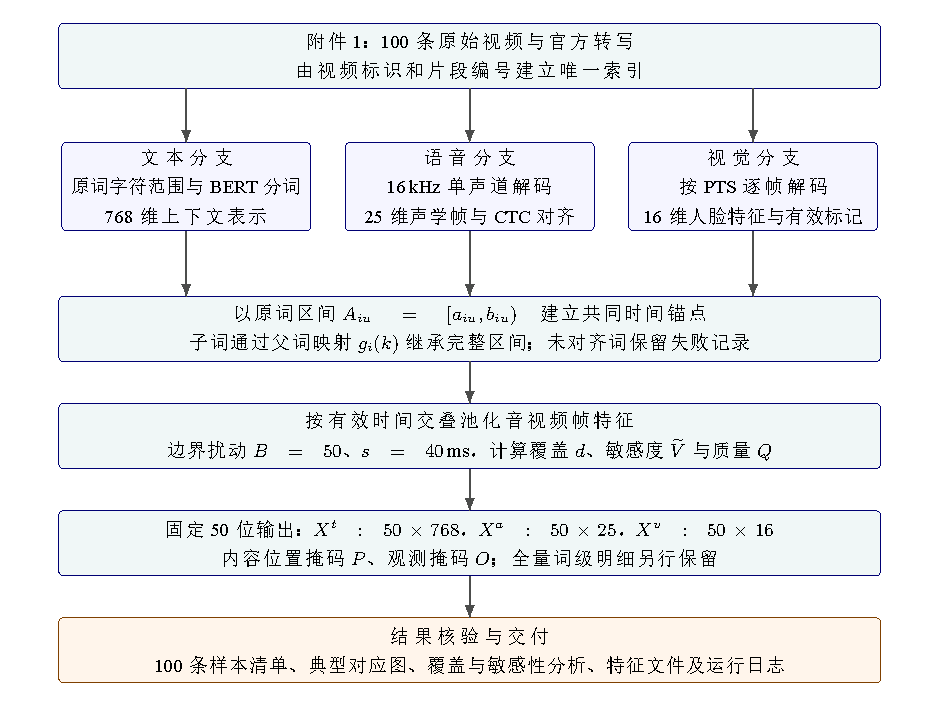
\includegraphics{figures/q1_flowchart.pdf}
\caption{三模态特征提取与时间锚点对齐流程}
\label{q1:fig:flow}
\end{figure}

模型输出采用50位定长接口，每个内容位置经父词索引关联至实际时间区间；模型评价从样本覆盖、区间结构、模态观测覆盖与参数敏感性四个方面展开。

\subsubsection{数据准备}
\label{q1:sec:data}

\paragraph{样本组织与数据特征}

附件1的样本以视频标识与片段编号组成唯一键，用于关联视频文件、官方转写与输出记录。100条样本来自37个原始视频，共含1932个空白分隔原词与2317个BERT词元；其中283个原词对应多个词元，占14.65\%。样本标签仅用于数据说明，不参与本问的特征提取与参数拟合。原始素材在文本长度、音频格式、视频采样、容器时间与可观测性上的实测特点及相应处理方式汇总于表\ref{q1:tab:data}。

输出按定长接口与全量记录两级组织：接口给出三模态共享的位置级输入，词级记录保留接口之外的时间对应与截断信息，两者通过父词索引相互关联。

\begin{table}[htbp]
\centering\small
\caption{数据特点与相应处理方式}
\label{q1:tab:data}
\begin{tabularx}{\linewidth}{p{3.1cm}p{4.0cm}Y}
\toprule
对象 & 实测特点 & 处理方式 \\
\midrule
文本长度 & 每条5--65词，5--82个词元 & 保存全量词表，固定接口仅保留前48个内容词元 \\
音频格式 & 源采样率44.1\,kHz，单/双声道AAC & 统一解码为16\,kHz单声道信号 \\
容器时间 & 90条声明帧数与实解帧数不同；声明33147帧、实解23241帧 & 区分媒体样本数、有效呈现时长与解码跨度 \\
有效呈现时长 & 100条样本各含一条编辑列表，视频与音频合计787.985\,s与777.106\,s & 逐样本以编辑列表限定的有效呈现时长汇总 \\
轨间时长差 & $\Delta_i=T_i^a-T_i^v$均值$-92.3$\,ms、绝对值中位数91.3\,ms & 随样本清单保存并用于范围核验，不作跨轨平移或重采样 \\
视频采样 & 8种分辨率，帧间隔并非处处均匀；实解帧的PTS完整且单调 & 使用逐帧PTS，不由帧数和标称帧率反推时间 \\
视觉可观测性 & 4条全片未检出人脸，另有局部未检出 & 保存有效帧掩码，缺失帧不参与池化 \\
\bottomrule
\end{tabularx}
\end{table}

\paragraph{时间基准与有效区间}

音频经解码、重采样与声道合并后得到信号 $x_i[n]$，采样率 $f_s=16000$\,Hz，其相对时间为 $n/f_s$；设解码样本数为 $N_i^a$，则音频轨的解码跨度 $T_i^a=N_i^a/f_s$。声学描述符提取与词级强制对齐共用该信号，以保证两条处理链具有一致的时间原点。

视频第 $j$ 帧的呈现时间取解码PTS与时间基的乘积，记为 $t_{ij}$，全部解码帧的PTS完整且单调。声明帧数与实解帧数存在明显差异，按标称帧率反推时间轴会把这一差异转成系统性的时间偏差，因此视觉时间支撑统一由实际解码帧的PTS建立，容器时间信息只用于确定有效呈现范围；视频轨的解码跨度 $T_i^v$ 按末帧PTS加一个中位帧间隔计算，与帧支撑的延展约定一致。

容器媒体时长、编辑列表时长与解码跨度分别描述存储范围、有效呈现范围与实际样本范围，三者的对照结果连同实解帧数与逐样本时长汇总于表\ref{q1:tab:data}与图\ref{q1:fig:dataset}。解码输出落在编辑列表限定的呈现范围内，逐样本汇总采用有效呈现时长；两轨解码跨度之差 $\Delta_i=T_i^a-T_i^v$ 随清单保存，用于范围核验，本文不对两条轨道作平移或重采样。


图\ref{q1:fig:dataset}给出样本长度与媒体时间分布：原词数呈长尾分布，故在定长接口之外保留全量词级记录；音视频解码跨度与帧数统计存在差异，故视觉分支采用实际解码帧与PTS建立时间支撑。

\begin{figure}[htbp]
\centering
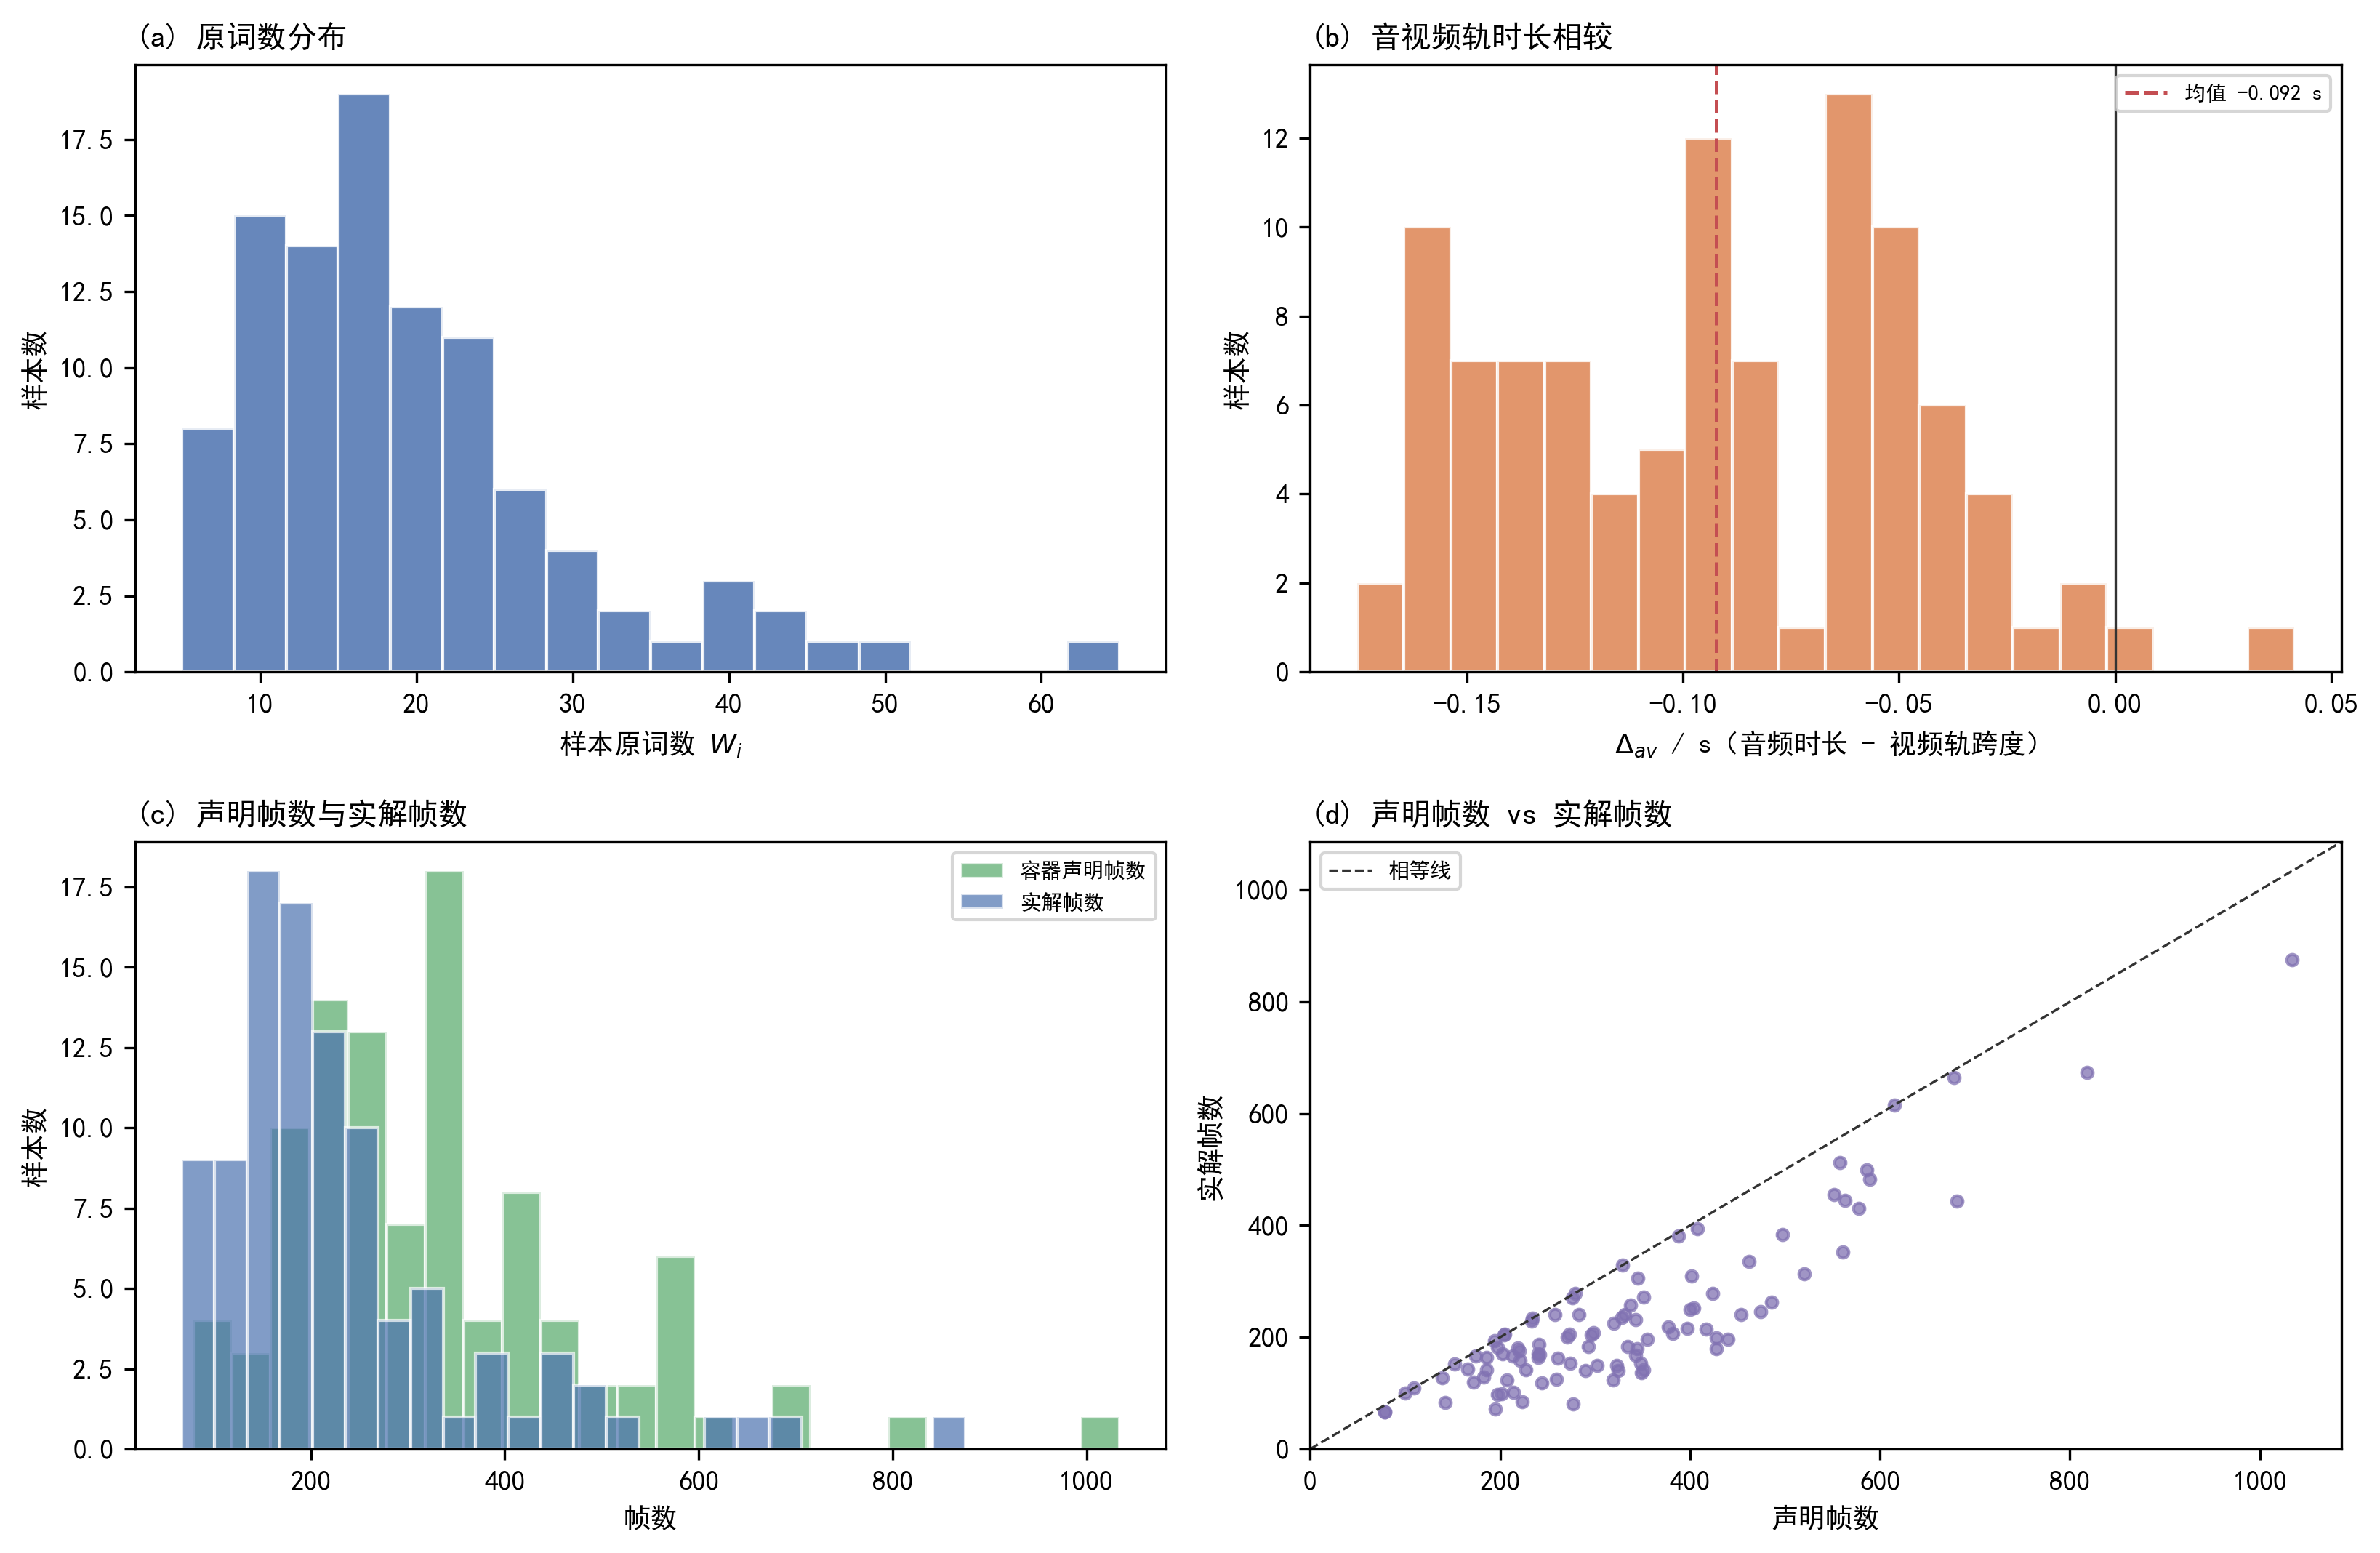
\includegraphics[width=\linewidth]{figures/q1_dataset.png}
\caption{附件1的原词数、音视频解码跨度差及帧数统计}
\label{q1:fig:dataset}
\end{figure}

\paragraph{建模约定}

本文以官方转写确定待对齐的词序列，同一原词的子词共享其时间区间；视觉描述符取自成功检出的人脸，质量分数用于评价锚点的相对可用性。各模态在词锚点上完成聚合后写入统一接口，内容掩码与观测掩码随特征一并保存；预训练模型保持冻结，分别承担特征编码与强制对齐，其参数计算不涉及附件1的情感标签。

\subsubsection{模型构建}
\label{q1:sec:model}

模型构建沿三条分支展开：文本分支确定位置级语义表示，语音分支给出词级时间区间，视觉分支提供帧级观测与有效性标记，三者在原词锚点上汇合为统一接口。位置、时间与观测三类信息分别由内容掩码 $P$、区间 $A_{iu}$ 与观测掩码 $O^m_{ik}$ 表达，使特征张量在存在局部缺失时仍保持明确的时间含义。

\paragraph{文本特征与词元归属}

文本情感通过评价对象、情感词、否定与程度修饰等语义单元表达，其时间定位依赖转写与音频的词级对应。转写以空白分词给出原词，预训练编码器以WordPiece为输入单位，两类单位在数量与边界上均不一致，因此先建立词元到原词的归属关系，再在同一接口内组织语义表示。

设原词 $w_{iu}$ 在转写中的字符范围为 $[l_{iu},r_{iu})$，分词器返回词元 $z_{ik}$ 的字符范围 $[l^z_{ik},r^z_{ik})$。若词元范围包含于原词范围内，定义
\begin{equation}
g_i(k)=u\quad\text{当}\quad
[l^z_{ik},r^z_{ik})\subseteq[l_{iu},r_{iu}).
\label{q1:eq:owner}
\end{equation}
对非包含关系，依次按字符交叠和邻词附着确定归属；本批100条样本均由包含关系确定父词。词内标点继承父词的时间区间，与所在原词共享同一时间锚点。

固定接口长度 $K=50$，顺序安排\file{[CLS]}、至多48个内容词元、\file{[SEP]}及尾部\file{[PAD]}。仅内容词元取 $P_{ik}=1$，其余位置为0。将包含特殊符号的完整接口输入BERT后，取最后一层隐藏向量：
\begin{equation}
X^t_{ik}=P_{ik}\bm h_{ik},\qquad \bm h_{ik}\in\R^{768}.
\label{q1:eq:text}
\end{equation}
内容掩码$P$排除特殊符号，BERT注意力掩码保留\file{[CLS]}和\file{[SEP]}，使内容位置的上下文表示涵盖完整句意。超过48个内容词元的尾部保存于全量词表，其父词继续参与音视频对齐与池化；位置级文本向量覆盖接口内的词元，接口之外的部分在词级记录中保持可追溯。编码器参数在本问中保持冻结，文本表示仅由原始转写决定。

\paragraph{语音特征与词级时间估计}

语音的响度、音高、谱形和发声质量能够表征重音、语调与发声方式，为情感分析提供区别于文字内容的线索。采用openSMILE的eGeMAPSv02低层描述符，获得25维帧特征 $\bm f^a_{ij}$，其分组与建模含义如表\ref{q1:tab:acoustic}所示。帧特征的时间区间直接取自工具输出，帧移为10\,ms、窗长为20\,ms，相邻窗口存在交叠，特征数值保持原始尺度进入聚合。

记第$j$个声学帧的工具输出支撑为$J^a_{ij}=[s^a_{ij},e^a_{ij})$。池化按该支撑区间计算交叠权重，保留分析窗的交叠关系；音频帧在整条样本内均记为有效观测。LLD提取与强制对齐共用16\,kHz单声道PCM信号，具有一致的时间原点。

\begin{table}[htbp]
\centering\small
\caption{声学特征的组成与建模含义（合计25维）}
\label{q1:tab:acoustic}
\begin{tabularx}{\linewidth}{>{\raggedright\arraybackslash}p{2.7cm}cY}
\toprule
特征组 & 维数 & 内容与作用 \\
\midrule
响度与谱形 & 6 & 响度、alpha比、Hammarberg指数、两个频段谱斜率、频谱通量，描述能量与频谱变化 \\
倒谱表示 & 4 & MFCC 1--4，描述短时谱包络 \\
基频与发声质量 & 6 & 基频半音值、jitter、shimmer、HNR及两项谐波相对能量，描述音高与声门发声特征 \\
共振峰 & 9 & 第一至第三共振峰的频率、带宽与相对幅度，描述声道共振结构 \\
\bottomrule
\end{tabularx}
\end{table}

词级时间估计将连续语音映射为离散词区间，采用预训练wav2vec2声学模型与CTC强制对齐完成。将原词映射为声学字典支持的大写字符，词间插入分隔符，构成目标序列 $\bm y_i$；无法产生目标字符的词保留为未对齐记录。设 $\pi_{it}(c)$ 为第 $t$ 个声学输出帧对字符 $c$ 的概率，最优路径为
\begin{equation}
\bm z_i^*=\arg\max_{\bm z:\,\mathcal B(\bm z)=\bm y_i}
\sum_t\log\pi_{it}(z_t),
\label{q1:eq:ctc}
\end{equation}
其中 $\mathcal B$ 表示CTC的去空白与重复合并映射；声学输出帧移 $h=0.02$\,s，各帧支撑按定长帧计算。对合并后的第 $c$ 个目标字符，记其帧支撑为 $[\alpha_{ic},\beta_{ic})$；原词包含的目标字符集合记为 $\mathcal C_{iu}$，则词区间为
\begin{equation}
A_{iu}=\left[h\min_{c\in\mathcal C_{iu}}\alpha_{ic},\ 
h\max_{c\in\mathcal C_{iu}}\beta_{ic}\right).
\label{q1:eq:word}
\end{equation}
式\eqref{q1:eq:word}使用字符支撑的起点与终点，允许字符之间存在空白帧，不假定字符连续占据整个词区间。强制对齐在给定转写顺序下搜索最优声学路径\cite{ref:ctc}。字符字典未覆盖的数字或符号保留为未对齐词；生成的词区间依次接受单调性、正长度和音轨边界检查，未通过检查的区间不计入有效锚点。

先对字符支撑内的路径对数概率求均值，再汇总原词中的各字符，定义词级路径置信度：
\begin{equation}
\bar\ell_{ic}=\frac{1}{\beta_{ic}-\alpha_{ic}}
\sum_{t=\alpha_{ic}}^{\beta_{ic}-1}\log\pi_{it}(y_{ic}),
\qquad
c_{iu}=\exp\left(\frac{1}{|\mathcal C_{iu}|}\sum_{c\in\mathcal C_{iu}}\bar\ell_{ic}\right).
\label{q1:eq:confidence}
\end{equation}
路径分数$c_{iu}$衡量声学模型对目标字符序列的支持程度，作为对齐质量分量进入综合评分；无法构造字符目标的词保留空区间，并单独记录可用性状态。

\paragraph{视觉特征与有效帧建模}

视觉分支提取人脸几何与关键点位移，用于表征口型、眼眉形态及面部运动，并以人脸尺度归一，使不同分辨率与人脸大小的样本具有可比的位移量度。先以FaceDetection定位最高分人脸，按人脸框宽高的1.6倍裁剪区域，再使用FaceMesh提取478个关键点；区域处理失败时尝试整帧检测。同一帧出现多张人脸时取检测分数最高者，作为该帧的目标人脸。将区域内坐标映射回原图后，取二维像素坐标 $\bm p_{ijq}=(x_{ijq},y_{ijq})$。对于宽$W$、高$H$的原帧，设裁剪边界为$(x_0,y_0,x_1,y_1)$，FaceMesh在裁剪图上返回归一化坐标$(u_{ijq},v_{ijq})$，则回映关系为
\begin{equation}
x_{ijq}=x_0+u_{ijq}(x_1-x_0),\qquad
y_{ijq}=y_0+v_{ijq}(y_1-y_0).
\label{q1:eq:roi-map}
\end{equation}
裁剪边界限制在$[0,W]\times[0,H]$内，关键点回映后在统一像素坐标系中计算跨帧位移。两阶段检测用于改善小人脸与高亮背景下的人脸可观测性，未检出帧通过有效性掩码记录。

以脸宽和脸高的均值作为尺度
\begin{equation}
L_{ij}=\frac{|x_{ij,234}-x_{ij,454}|+|y_{ij,10}-y_{ij,152}|}{2}+10^{-6},
\qquad
\delta_{ij}(p,q)=\frac{\|\bm p_{ijp}-\bm p_{ijq}\|_2}{L_{ij}},
\label{q1:eq:face-scale}
\end{equation}
构造表\ref{q1:tab:vision}中的14个几何分量及2个运动分量，分别描述眼眉口部形态和关键点位移。取相邻帧 $j-1$ 与 $j$，且两帧均成功检出人脸，对全脸或嘴部关键点集合 $\mathcal P$ 定义运动量
\begin{equation}
M_{ij}(\mathcal P)=\sqrt{\frac{1}{|\mathcal P|}
\sum_{q\in\mathcal P}\frac{\|\bm p_{ijq}-\bm p_{i,j-1,q}\|_2^2}{L_{ij}^2}}.
\label{q1:eq:motion}
\end{equation}
首帧或前一帧未检出人脸时运动不可测，该帧记无效并存储零向量，不以前一有效帧的关键点替代；不可测原因（首帧、跨检测缺口）在帧级文件与样本元数据中分别记录。

\begin{table}[htbp]
\centering\small
\caption{16维视觉描述符的定义}
\label{q1:tab:vision}
\begin{tabularx}{\linewidth}{cp{3.0cm}Y}
\toprule
维度 & 描述符 & 定义 \\
\midrule
1--3 & 嘴开合、嘴宽、开合宽比 & $\delta(13,14)$、$\delta(61,291)$及$\delta(13,14)/(\delta(61,291)+10^{-6})$ \\
4--5 & 左右嘴角相对高度 & 上下唇中点纵坐标减嘴角61或291的纵坐标，再除以 $L$ \\
6--7 & 左右眼开合 & $\delta(159,145)$、$\delta(386,374)$ \\
8--9 & 左右眼宽 & $\delta(33,133)$、$\delta(362,263)$ \\
10--11 & 左右眉眼距离 & $\delta(105,159)$、$\delta(334,386)$ \\
12--13 & 补充眉眼距离 & $\delta(70,159)$、$\delta(300,386)$ \\
14 & 脸高宽比 & $|y_{10}-y_{152}|/(|x_{234}-x_{454}|+10^{-6})$ \\
15--16 & 全脸与嘴部位移 & 相邻两帧均检出时的归一化关键点位移RMS；不可测帧不进入池化 \\
\bottomrule
\end{tabularx}
\end{table}

视觉帧的有效标记 $r^v_{ij}=1$ 要求相邻两帧均检出；人脸未检出或运动不可测时置 $r^v_{ij}=0$ 并存储零向量。帧的支撑区间定义为
\begin{equation}
J^v_{ij}=[t_{ij},t_{i,j+1}),\quad j<N_i^v;
\qquad J^v_{i,N_i^v}=[t_{i,N_i^v},t_{i,N_i^v}+\widehat h_i^v),
\label{q1:eq:video-time}
\end{equation}
其中 $\widehat h_i^v$ 为正帧间隔的中位数。该约定将当前帧描述符保持到下一帧，在帧间隔较大时包含保持近似；视觉覆盖指标据此衡量有效视觉帧对锚点区间的支撑程度。

\paragraph{时间交叠池化与子词映射}

不同模态无须先统一帧率：词锚点给出统一的时间窗口，各模态按自身帧支撑进入窗口完成聚合。对词区间 $A=[a,b)$，令有效交叠长度为
\begin{equation}
\ell^m_{ij}(A)=r^m_{ij}\max\{0,\min(b,e^m_{ij})-\max(a,s^m_{ij})\},
\quad S^m_i(A)=\sum_j\ell^m_{ij}(A),
\label{q1:eq:overlap}
\end{equation}
音频帧取 $r^a_{ij}=1$，视觉使用检测有效性。若 $S^m_i(A)>\varepsilon$，则
\begin{equation}
\omega^m_{ij}(A)=\frac{\ell^m_{ij}(A)}{S^m_i(A)},\quad
\bm x^m_{iu}=\sum_j\omega^m_{ij}(A_{iu})\bm f^m_{ij},\quad
d^m_{iu}=\min\left(1,\frac{S^m_i(A_{iu})}{b_{iu}-a_{iu}}\right),
\label{q1:eq:pool}
\end{equation}
其中 $\varepsilon=10^{-9}$。无有效交叠时，令 $\bm x^m_{iu}=\bm0$、$d^m_{iu}=0$。式\eqref{q1:eq:pool}使部分交叠的帧按实际支撑长度贡献特征，权重归一化与覆盖指标分开计算，在归一化权重的同时保留缺失程度的信息；声学分析窗存在交叠，$d^a$按有效交叠长度累计并截断到1。

图\ref{q1:fig:overlap}给出一组可手算的视觉例子。设词区间为$[0.08,0.32)$\,s，四个相邻帧支撑各长0.10\,s，第三帧未检出人脸，则四帧有效交叠依次为$0.02,0.10,0,0.02$\,s。由式\eqref{q1:eq:pool}，非零权重为$1/7,5/7,1/7$，而覆盖指标为$0.14/0.24=0.583$。即使权重和为1，词区间仍有$41.7\%$的时长缺乏有效视觉支撑；这正是单独保存$d^v$的必要性。
\begin{figure}[htbp]
\centering
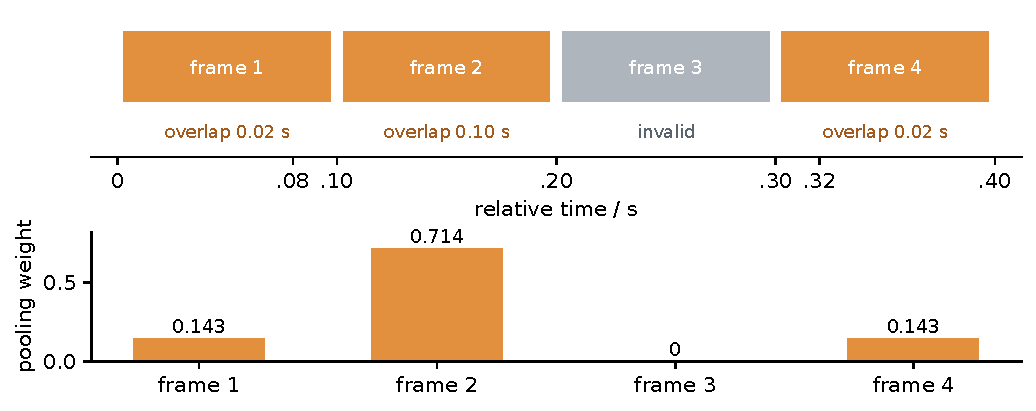
\includegraphics[width=0.92\linewidth]{figures/q1_overlap_example.pdf}
\caption{交叠池化示意算例}
\label{q1:fig:overlap}
\end{figure}

通过父词映射，将音视频词级特征复制到对应子词位置：
\begin{equation}
X^m_{ik}=\begin{cases}\bm x^m_{i,g_i(k)},&P_{ik}=1,\\\bm0,&P_{ik}=0,\end{cases}
\quad
O^m_{ik}=P_{ik}\ind\{d^m_{i,g_i(k)}>0\},\qquad m\in\{a,v\}.
\label{q1:eq:anchor}
\end{equation}
非内容位置的 $O$ 定义为0，不求值不存在的父词。三模态最终维度分别为
\begin{equation}
X^t_i\in\R^{50\times768},\qquad
X^a_i\in\R^{50\times25},\qquad
X^v_i\in\R^{50\times16}.
\end{equation}
多个子词继承父词的完整区间，不等分原词时间；同一原词的各子词共享相同的池化向量、覆盖指标与质量分量，记$Q^m_{ik}=Q^m_{i,g_i(k)}$，非内容位置不定义；位置级输出与词级时间记录由此一一对应。$P=1,O^m=0$表示位置存在但该模态无观测，与全零特征在模型中由内容掩码和观测掩码分别表达。

\paragraph{边界扰动与质量分量}

词边界由强制对齐给出，边界的小幅变化会改变参与聚合的帧及其权重。为刻画这一影响，对区间两端加入标准差$s=40$\,ms的独立高斯扰动，采样$B=50$次并重新池化；扰动幅度小于多数词区间的时长，用于刻画小范围边界移动的影响。两端先裁剪到模态时间范围；若终点不大于起点，设置20\,ms的最小区间。池化使用修正区间与有效帧的实际交叠，完全无覆盖的扰动另行计数。

令 $\mathcal H^m_{iu}$ 为有覆盖的扰动集合，$B^m_{iu}=|\mathcal H^m_{iu}|$。当 $B^m_{iu}\ge2$ 时定义
\begin{align}
\bar{\bm x}^{m,\mathrm{pert}}_{iu}&=\frac{1}{B^m_{iu}}\sum_{q\in\mathcal H^m_{iu}}\bm x^{m,(q)}_{iu},\\
V^m_{iu}&=\frac{1}{B^m_{iu}}\sum_{q\in\mathcal H^m_{iu}}
\left\|\bm x^{m,(q)}_{iu}-\bar{\bm x}^{m,\mathrm{pert}}_{iu}\right\|_2^2.
\label{q1:eq:variance}
\end{align}
原窗口无观测或有效扰动不足2次时，设置退化标记，方差字段以0占位；其余锚点的$V$衡量有观测条件下的边界敏感性，有效扰动次数$B^m_{iu}$随结果保存。

在每条样本内部，按有效帧计算模态尺度
\begin{equation}
\sigma_{im}^2=\frac{1}{N^{m,\mathrm{valid}}_i}\sum_{j:r^m_{ij}=1}
\|\bm f^m_{ij}-\bar{\bm f}^m_i\|_2^2+10^{-12},
\qquad \vt^m_{iu}=\frac{V^m_{iu}}{\max(\sigma_{im}^2,10^{-9})}.
\label{q1:eq:scale}
\end{equation}
少于2个有效帧时，尺度取1。归一化方差刻画池化变化相对于片段内特征变化的大小，各模态分别统计。

综合质量分数取
\begin{equation}
Q^m_{iu}=c_{iu}\,d^m_{iu}\exp(-\gamma_m\vt^m_{iu}),\qquad \gamma_a=\gamma_v=1.
\label{q1:eq:quality}
\end{equation}
路径置信度、观测覆盖与边界敏感性分别从对齐可信度、观测完整性和边界稳健性三个方面刻画锚点，共同决定综合质量$Q$。保存$c,d,V,\vt,Q$及退化标记，可按质量排序定位待复核锚点，并追溯相应的影响分量。

三项分量相乘给出明确的边界行为：词对齐失败时没有可用锚点；锚点存在但人脸完全缺失时$d^v=0$，因而$Q^v=0$；有覆盖且扰动能够产生至少两个有效池化结果时，边界敏感性有可解释的估计。零覆盖与低稳定性属于不同状态，逐词记录中的观测掩码与退化标记用于区分二者。
\subsubsection{模型求解与参数设置}
\paragraph{求解流程}

全部特征与时间映射在冻结预训练模型的条件下逐样本求解，网络参数不参与更新，输出由输入素材与固定参数共同决定。

\begin{enumerate}
\item 读取样本标识与官方转写，建立原词字符区间及其词元归属，生成文本特征与50位内容掩码。
\item 解码音轨，提取25维声学帧特征；对全量原词构建字符目标，计算CTC路径、词区间与路径置信度。
\item 按视频PTS读取帧，计算16维人脸特征与有效帧掩码，并建立各帧的支撑区间。
\item 对每个已生成区间的原词执行交叠池化与边界扰动；未生成区间的词保留失败记录，不赋予人为时间。
\item 将词级特征映射到保留的子词位置，输出特征、掩码与质量分量，并保存全量词表及截断尾部记录。
\item 汇总100条样本，核查样本键、张量形状、区间顺序与有效范围，生成全量清单与典型对应图。
\end{enumerate}

\paragraph{工具与关键参数}

扰动随机种子由样本标识的MD5摘要前8位生成，固定 $B,s,\gamma$ 后可在同一运行环境中复算。各分支所用工具、版本与关键设置见表\ref{q1:tab:environment}。

\begin{table}[htbp]
\centering\small
\caption{特征提取工具与关键参数}
\label{q1:tab:environment}
\begin{tabularx}{\linewidth}{p{2.3cm}p{4.4cm}Y}
\toprule
模块 & 工具及版本 & 设置 \\
\midrule
运行环境 & Python 3.12.10，CPU & NumPy 1.26.4，pandas 2.3.3 \\
音视频解码 & PyAV 18.1.0 & 音频16\,kHz单声道，视觉采用解码PTS \\
文本编码 & transformers 4.56.0 & \file{bert-base-uncased}，推理模式，50位 \\
声学描述符 & openSMILE 2.6.0 & eGeMAPSv02，LLD层，25维 \\
词级对齐 & torch / torchaudio 2.8.0 & \file{WAV2VEC2\_ASR\_BASE\_960H}，20\,ms帧移 \\
人脸描述符 & MediaPipe 0.10.21 & FaceDetection与FaceMesh，478点，ROI倍率1.6 \\
边界扰动 & NumPy随机生成器 & $B=50$，$s=40$\,ms，$\gamma_a=\gamma_v=1$ \\
\bottomrule
\end{tabularx}
\end{table}

逐样本运行记录的累计处理耗时约9.7\,min，其中视觉分支占85.6\%：人脸检测与关键点回归需逐帧执行，构成耗时的主要部分，逐阶段耗时随运行日志保存。自生成特征文件的存储格式、组织结构与读取方式见附录\ref{app:q1-files}。

\subsubsection{实验结果与分析}
\label{q1:sec:results}

\paragraph{全量处理结果与统计口径}

100条样本的1932个原词中，1920个生成时间区间，生成率为99.38\%，已生成区间在时间轴上构成随词序单调递增的分段覆盖（表\ref{q1:tab:all100}）。四项结构条件：非负起点、正长度、音轨范围内终点与起点随词序单调，在全部已生成区间上均无违例，说明对齐结果不存在跨越词序或越过音轨边界的失序情形。未生成的12项由数字词与标点符号串构成，其声学读法本身不稳定，字符目标无法可靠构造，失败记录被保留而未赋予人为时间。


声学特征在每个已生成区间内都有实际帧支撑；视觉覆盖均值为0.9276，低于1.000的部分来自人脸未检出与运动不可测帧，而不是时间区间缺失（图\ref{q1:fig:coverage-summary}）。路径置信度呈双峰分布，均值明显低于中位数，说明少量声学支持较弱的锚点把均值拉低，这部分锚点的区间时长也偏长；质量分量因此把置信度、覆盖与边界敏感性分开记录，使待复核锚点可按分量追溯，而不是只给出一个综合分数。

在固定接口中，未生成时间区间的词仍然保留内容位置，其文本语义可以参与判别而时间支撑为零，三态表示据此把“有文本、无时间支撑”与“文本、时间支撑齐备”两类位置区分开。视觉方面，另有128个已生成区间的词没有获得有效视觉支撑，有样本全片未检出人脸；帧级记录把未检出与运动不可测分别计数，这些帧不进入池化。时间区间是否有效与人脸观测是否有效是两个独立条件，在模型中分别由内容掩码与观测掩码表达。

已生成区间的词长普遍较短且长短相差较大，按词数均分音轨会把词间停顿摊入相邻词，并掩盖短词的真实边界；CTC对齐给出的边界落在声学证据上，交叠池化按实际帧支撑计算，两者共同保证短词与停顿处的特征归属不被平均化。


图\ref{q1:fig:coverage-summary}从词元保留与词级观测状态两个角度分解接口覆盖的构成：内容词元的接口保留比例为96.98\%，未进入接口的词元来自长文本截断，其词级时间与特征记录仍完整保留；音频的零覆盖全部出现在未生成时间区间的词上，视觉的零覆盖则发生在已生成区间内部，两类缺口的来源在图中可以直接区分。
\begin{figure}[htbp]
\centering
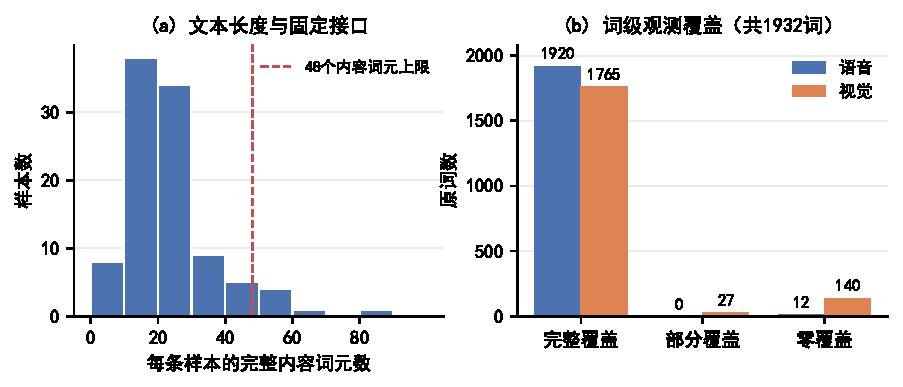
\includegraphics[width=0.9\linewidth]{figures/q1_coverage_summary.pdf}
\caption{接口覆盖情况}
\label{q1:fig:coverage-summary}
\end{figure}

\paragraph{典型样本的文本、语音与视频对应}

选取样本\file{-yRb-Jum7EQ\$\_\$5}。该句以否定与转折改变语义走向：\textit{not by the students of terrorism, but by those who teach terrorism}；三类模态在该片段内均有观测，语义转折处伴随可核验的韵律变化，适合用于展示跨模态对应关系。图\ref{q1:fig:typical}在统一秒轴上按五个面板给出对应关系。面板(a)为语音波形与25个原词的词级区间，红色窗标记否定与转折词，点线为切分词\textit{not}的6.37\,s时刻；面板(b)给出基频与能量曲线，切分点前后的中位数相差$1.2$半音，否定与转折词处出现局部峰；面板(c)为五个关键帧，按解码PTS定位，其中一帧落在切分时刻；面板(d)与面板(e)分别为25维声学帧特征与16维视觉帧特征，按维度标准化后与前三个面板共用同一时间轴，视觉热图中的空白对应无效视觉帧。

\begin{figure}[htbp]
\centering
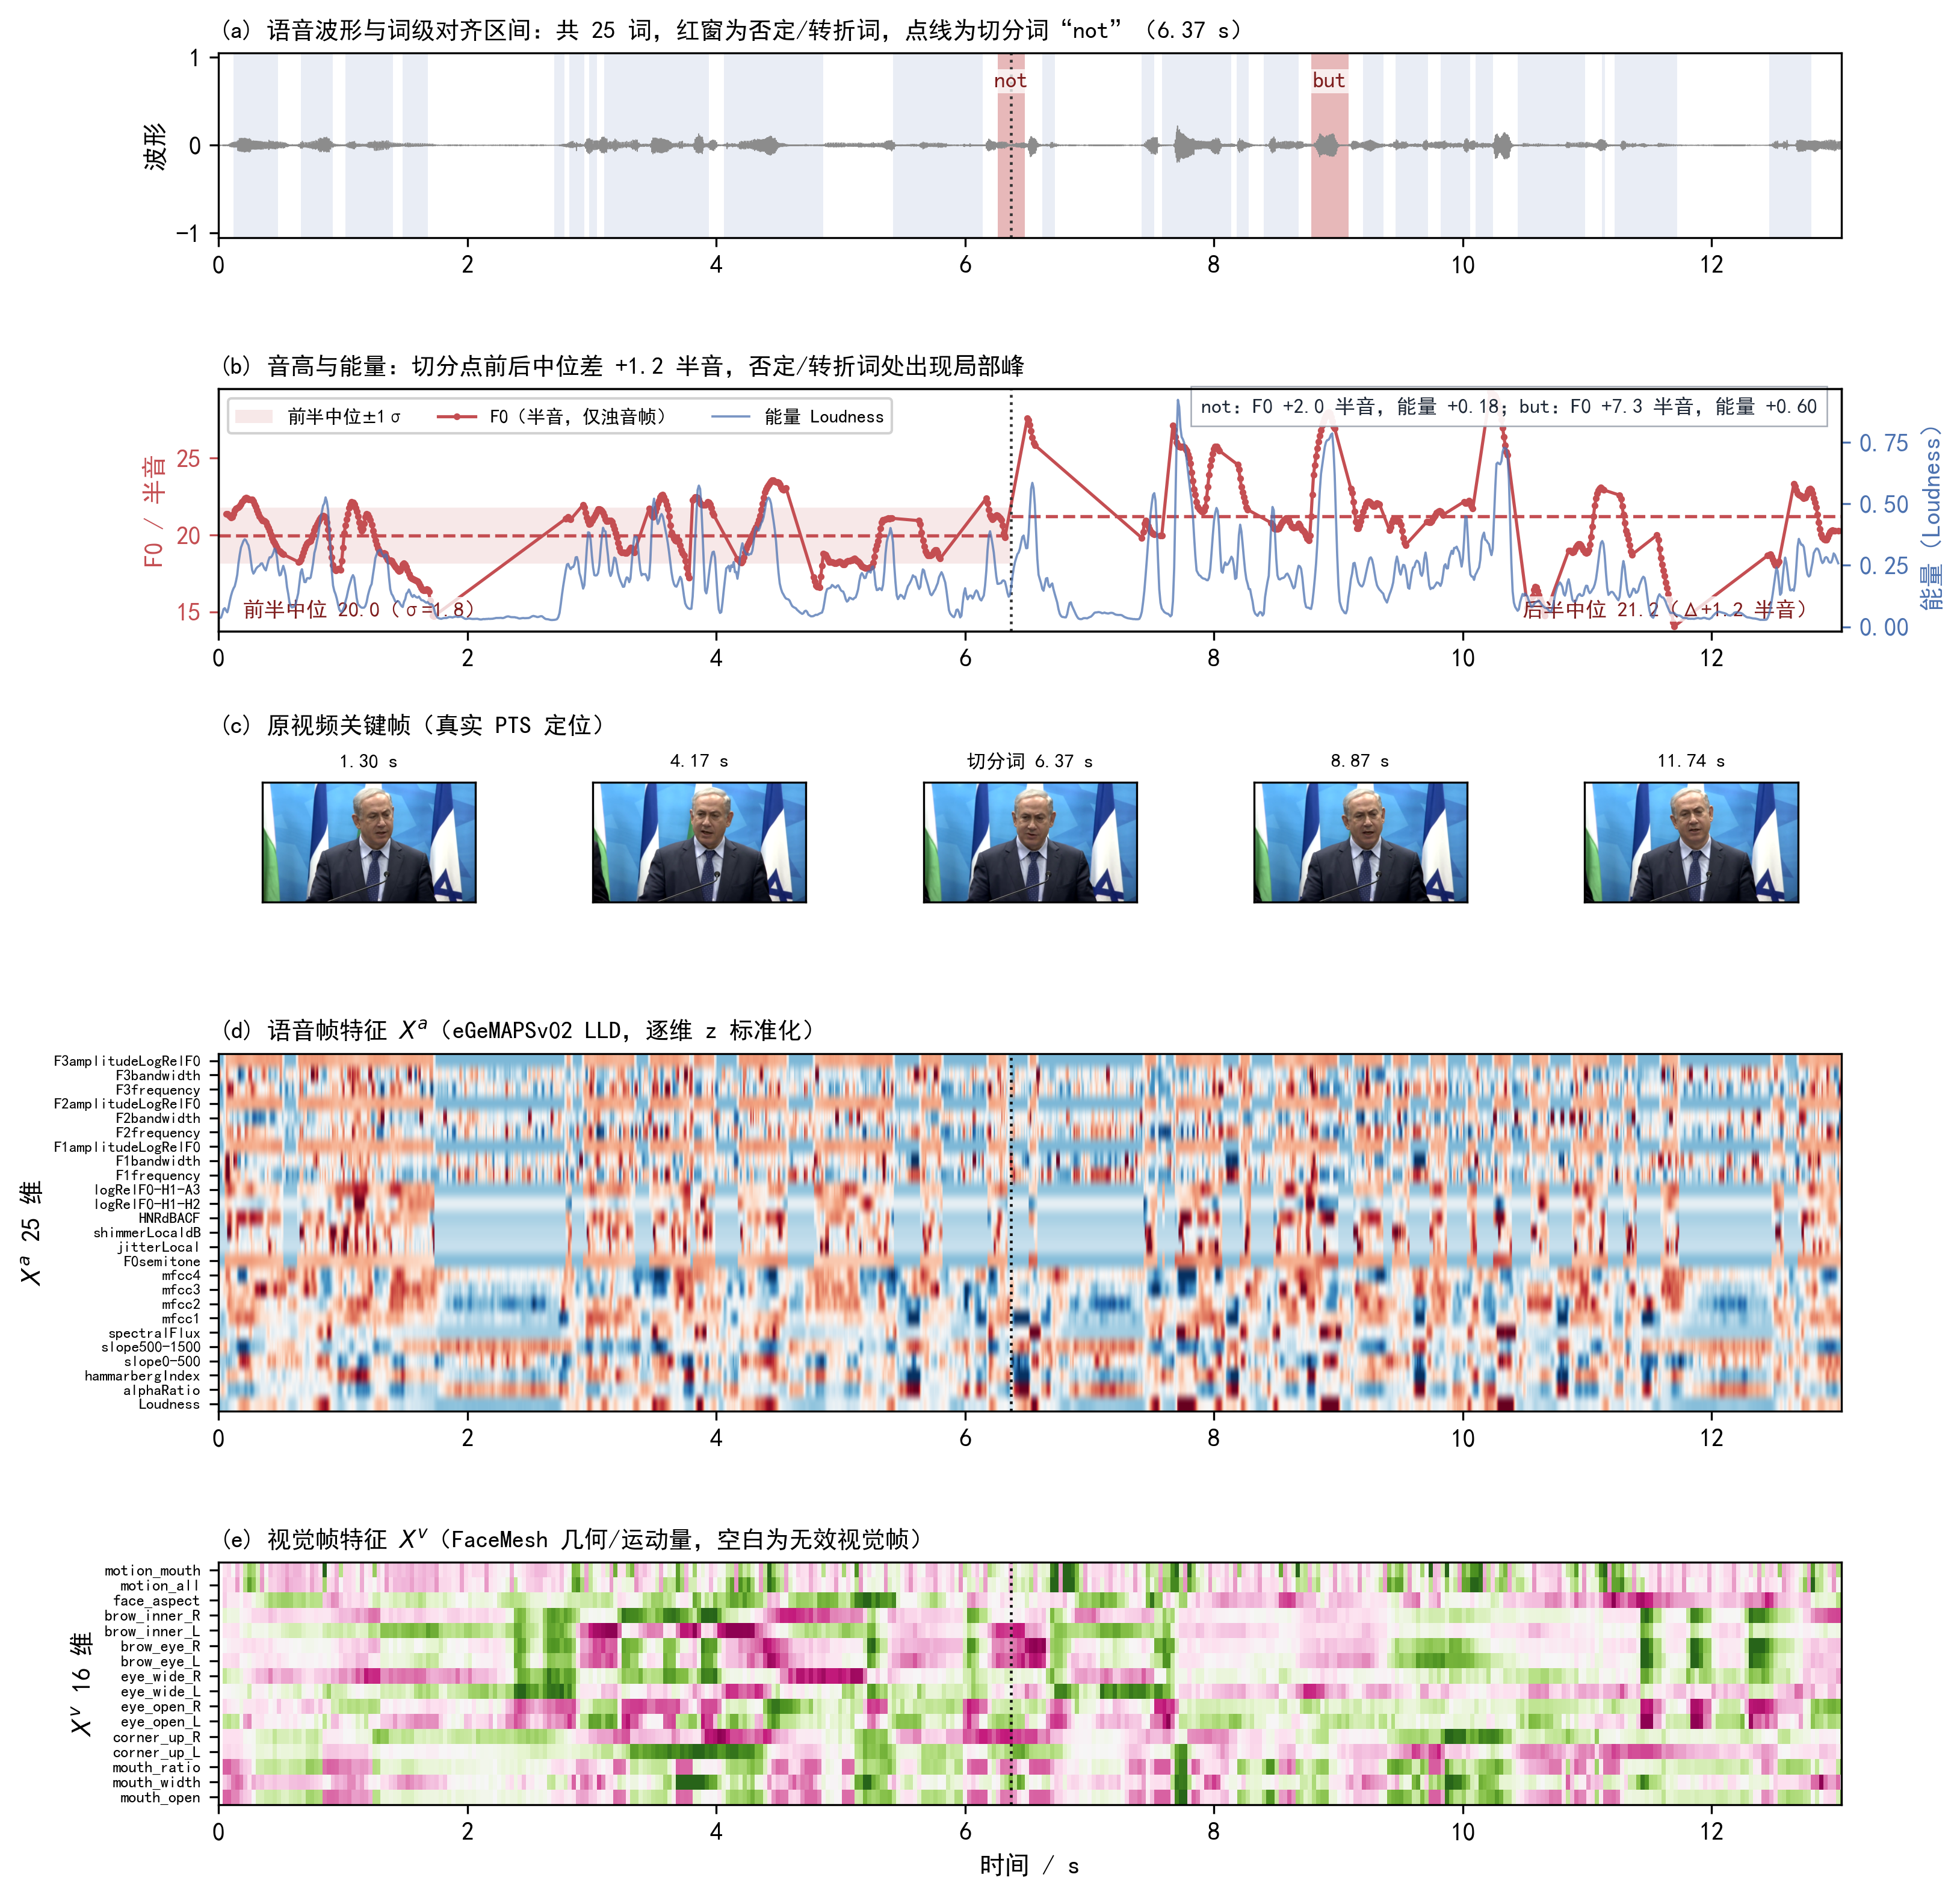
\includegraphics[width=\linewidth]{figures/q1_fig8_typical_correspondence.png}
\caption{典型样本的文本、语音与视频对应}
\label{q1:fig:typical}
\end{figure}

表\ref{q1:tab:typical}给出所选词的语音区间、词元数以及词处的音高与能量，这些词的音频与视觉覆盖均为1.00。以\file{teacher.}为例，父词区间为$[12.46,12.80)$\,s，两个词元共享该区间，分别对应768维上下文文本表示，并继承相同的音视频池化向量。否定与转折处出现局部音高与能量峰值：\textit{not}与\textit{but}相对各自前段参考窗口分别抬高$2.0$与$7.3$半音，能量同步抬升。在100条样本内可评估的20个否定/转折词上（所在样本人脸检出率不低于0.95且对齐词数不少于8），多数出现音高局部抬高、中位抬高$2.2$半音，全部出现能量抬升。词元语义、语音窗口与视频帧段由此在同一时间轴上建立一致对应，否定与转折的韵律标记落在同一位置。同一父词的多个词元共享音视频池化结果、同时保留各自的上下文文本表示，时间对齐定义在词与音频、视频之间，语义编码定义在子词位置，两种粒度在接口中互不干扰。文本向量由这些词对应的内容位置取得，视频帧通过PTS定位，不由50位下标换算时间。



\begin{table}[htbp]
\centering\small
\caption{典型样本的词区间与三模态映射}
\label{q1:tab:typical}
\begin{tabular}{lcccc}
\toprule
原词 & 语音区间(s) & 词元数 & $F_0$ (半音) & 能量 \\
\midrule
\texttt{lost} & [1.48, 1.68) & 1 & 18.1 & 0.14 \\
\texttt{attack,} & [5.42, 6.14) & 2 & 20.3 & 0.21 \\
\texttt{not}$^{\dagger}$ & [6.26, 6.48) & 1 & 21.2 & 0.34 \\
\texttt{but}$^{\dagger}$ & [8.78, 9.08) & 1 & 27.9 & 0.76 \\
\texttt{teach} & [10.10, 10.24) & 1 & 29.3 & 0.36 \\
\texttt{teacher.} & [12.46, 12.80) & 2 & 23.0 & 0.33 \\
\bottomrule
\end{tabular}
\end{table}
\paragraph{观测缺失与截断的处理效果}

图\ref{q1:fig:missing}展示一条视觉观测中途缺失的样本\file{-HwX2H8Z4hY\$\_\$5}：该片为人物近景与字幕图形叠加的镜头，未检出区间的人脸呈侧转姿态并与字幕重叠。该样本多数锚点没有有效视觉支撑，仅前两个词保有视觉帧，其余锚点取$O^v=0$、$Q^v=0$；这些位置的音频分量仍由声学帧独立给出，文本表示保持完整。该例说明位置级掩码把缺失限定在发生缺口的词与模态上：视觉观测的缺口不改动其余锚点的时间对应，也不向音频与文本扩散。

\begin{figure}[htbp]
\centering
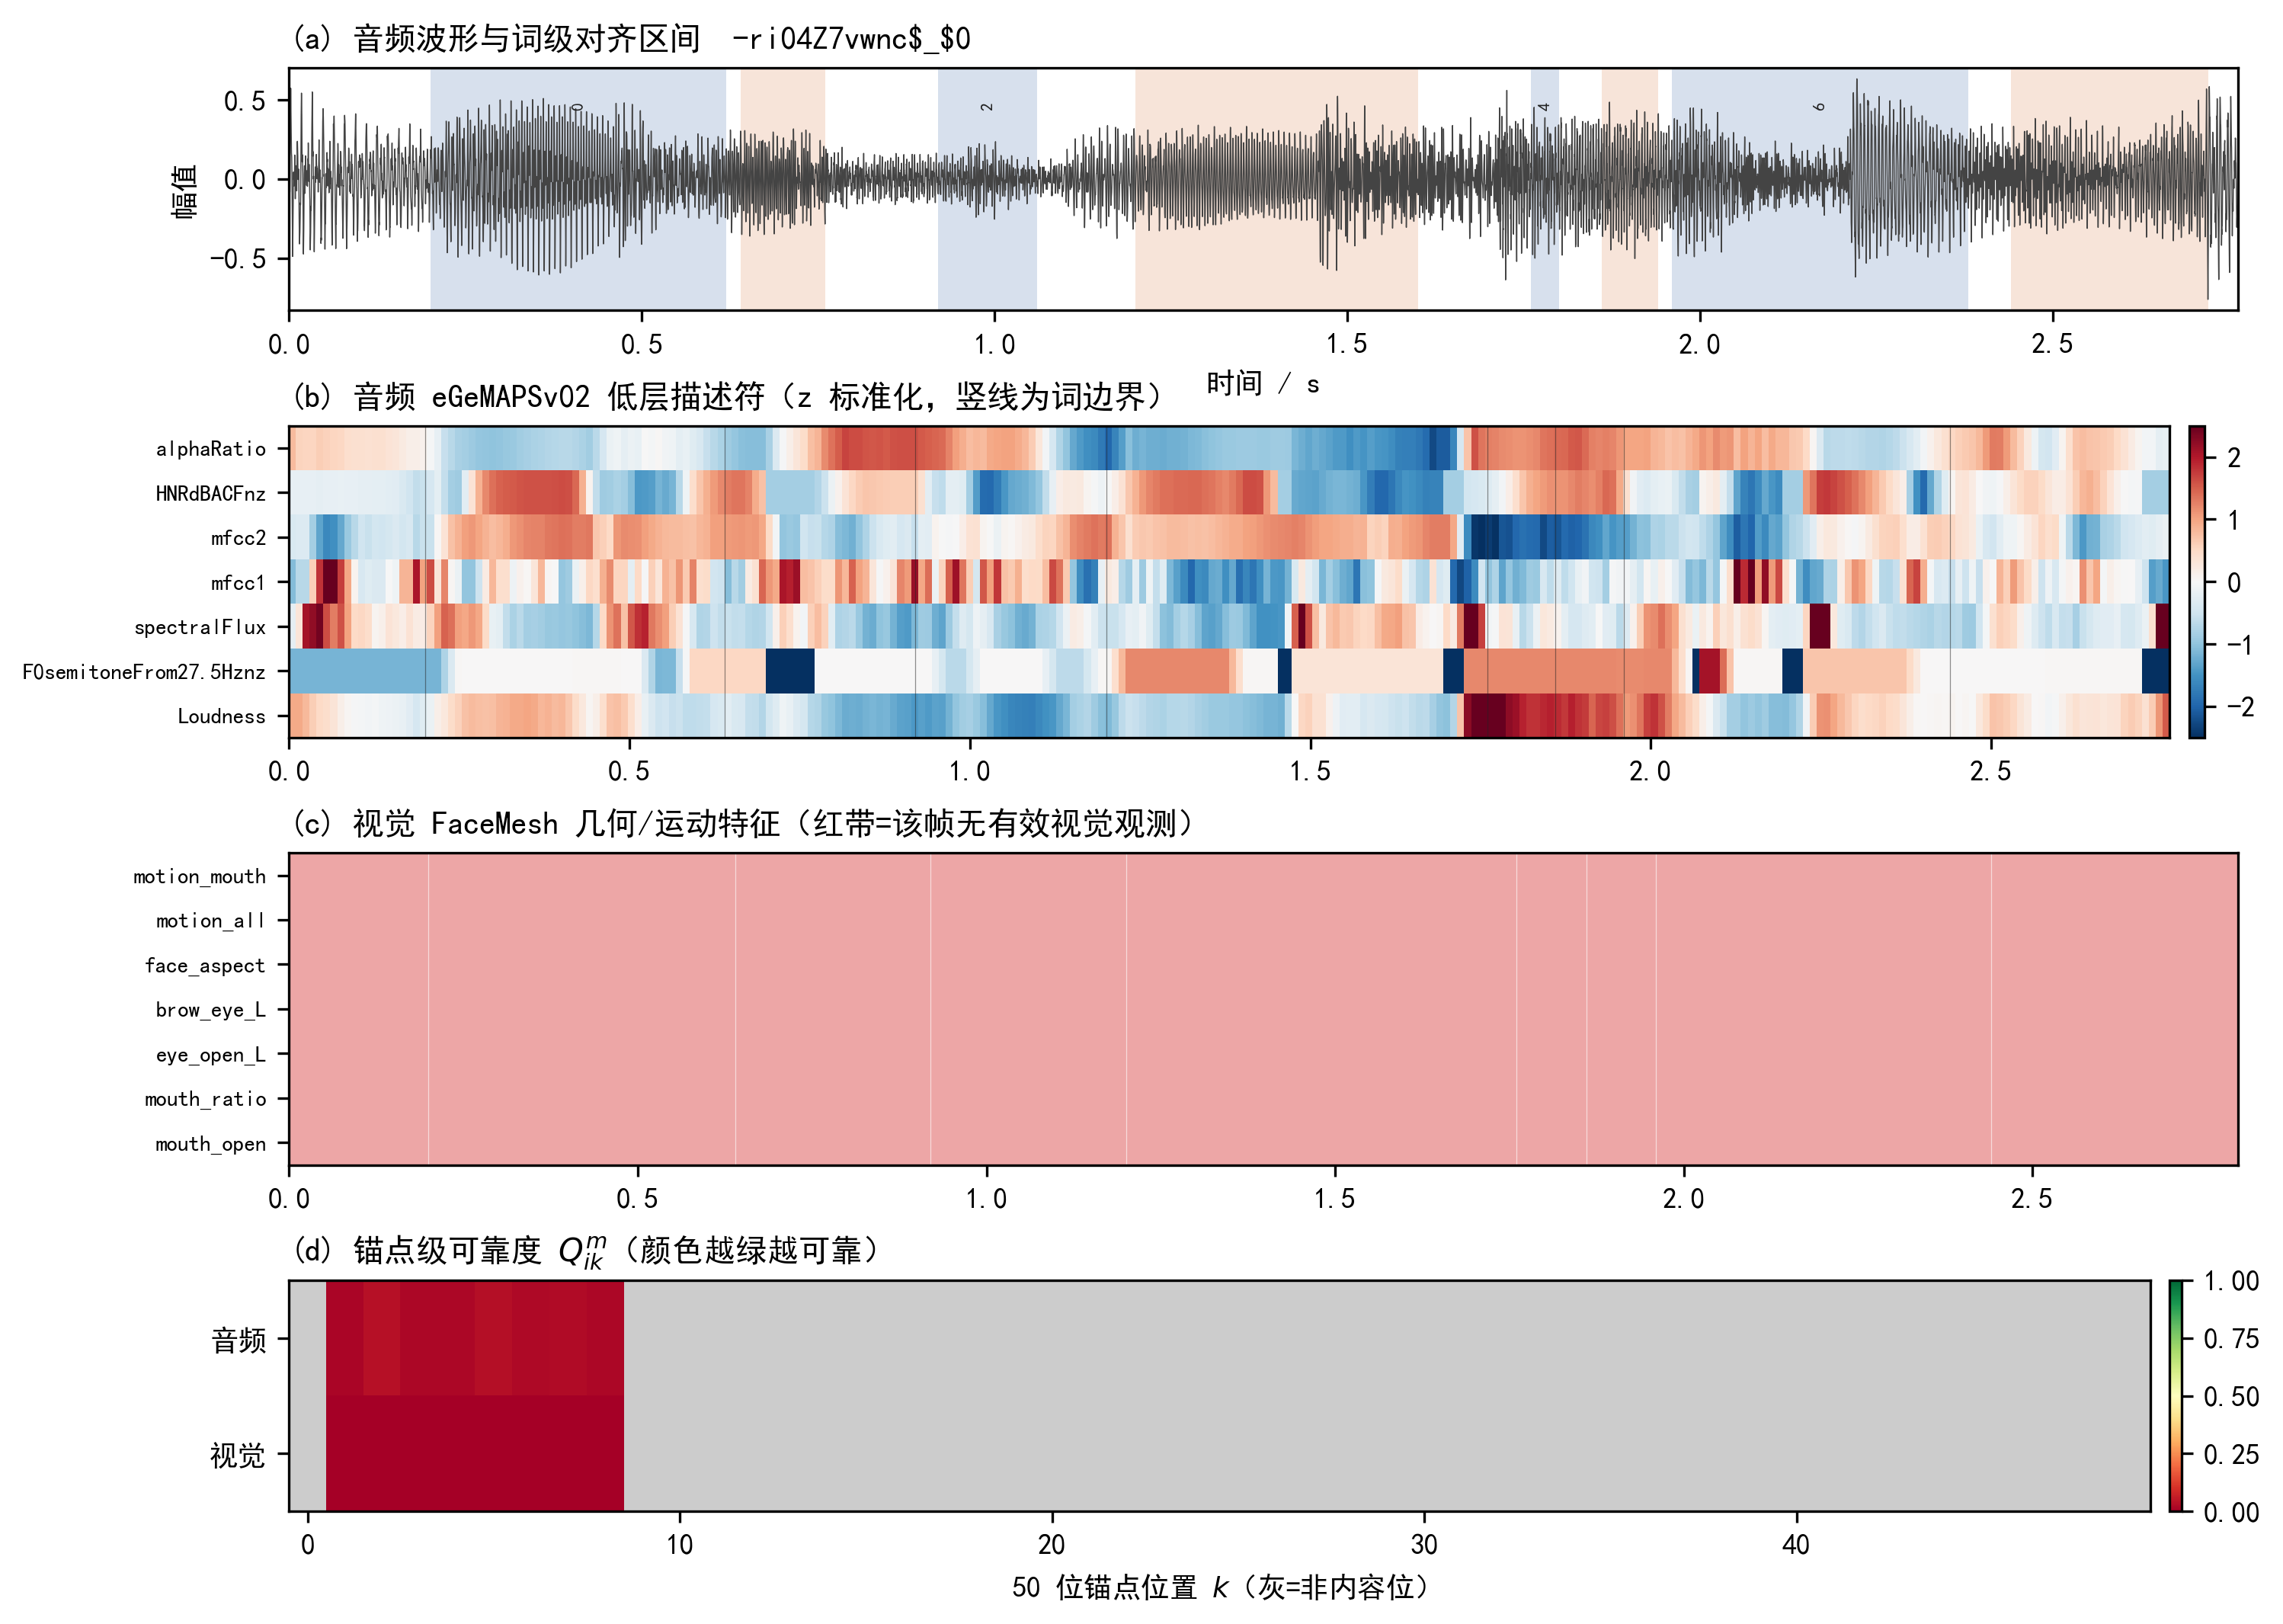
\includegraphics[width=0.91\linewidth]{figures/q1_fig1_overview_missing.png}
\caption{局部视觉观测缺失样本}
\label{q1:fig:missing}
\end{figure}

文本方面，6条样本的内容词元超过48个的接口上限；在最严重的一条中，前39个原词即占满全部内容位，其余原词的词元在接口中没有位置，但其词级区间与音视频池化记录仍按原顺序保留。截断只改变进入接口的词元数量，不改变词级时间记录。

\paragraph{质量分量与参数敏感性}


综合质量的均值低于中位数，低值部分由零覆盖锚点的$Q=0$贡献，中位数更能代表多数锚点的水平：音频与视觉的质量中位数都在0.87以上，视觉更高。视觉边界的相对波动低于音频，零覆盖词另记为退化状态；音视频$Q$在样本内保持一致的排序趋势，排序差异来自各自独立的覆盖与扰动分量，这一结构使质量分量既可用于整体排序，也可用于分量层面的复核。

图\ref{q1:fig:quality}给出三个分量的分布与音视频$Q$的联合分布：相同覆盖率的锚点因路径置信度不同而具有不同质量，零覆盖词的$Q$落在零点，边界扰动的差异在对数坐标下展开。
\begin{figure}[htbp]
\centering
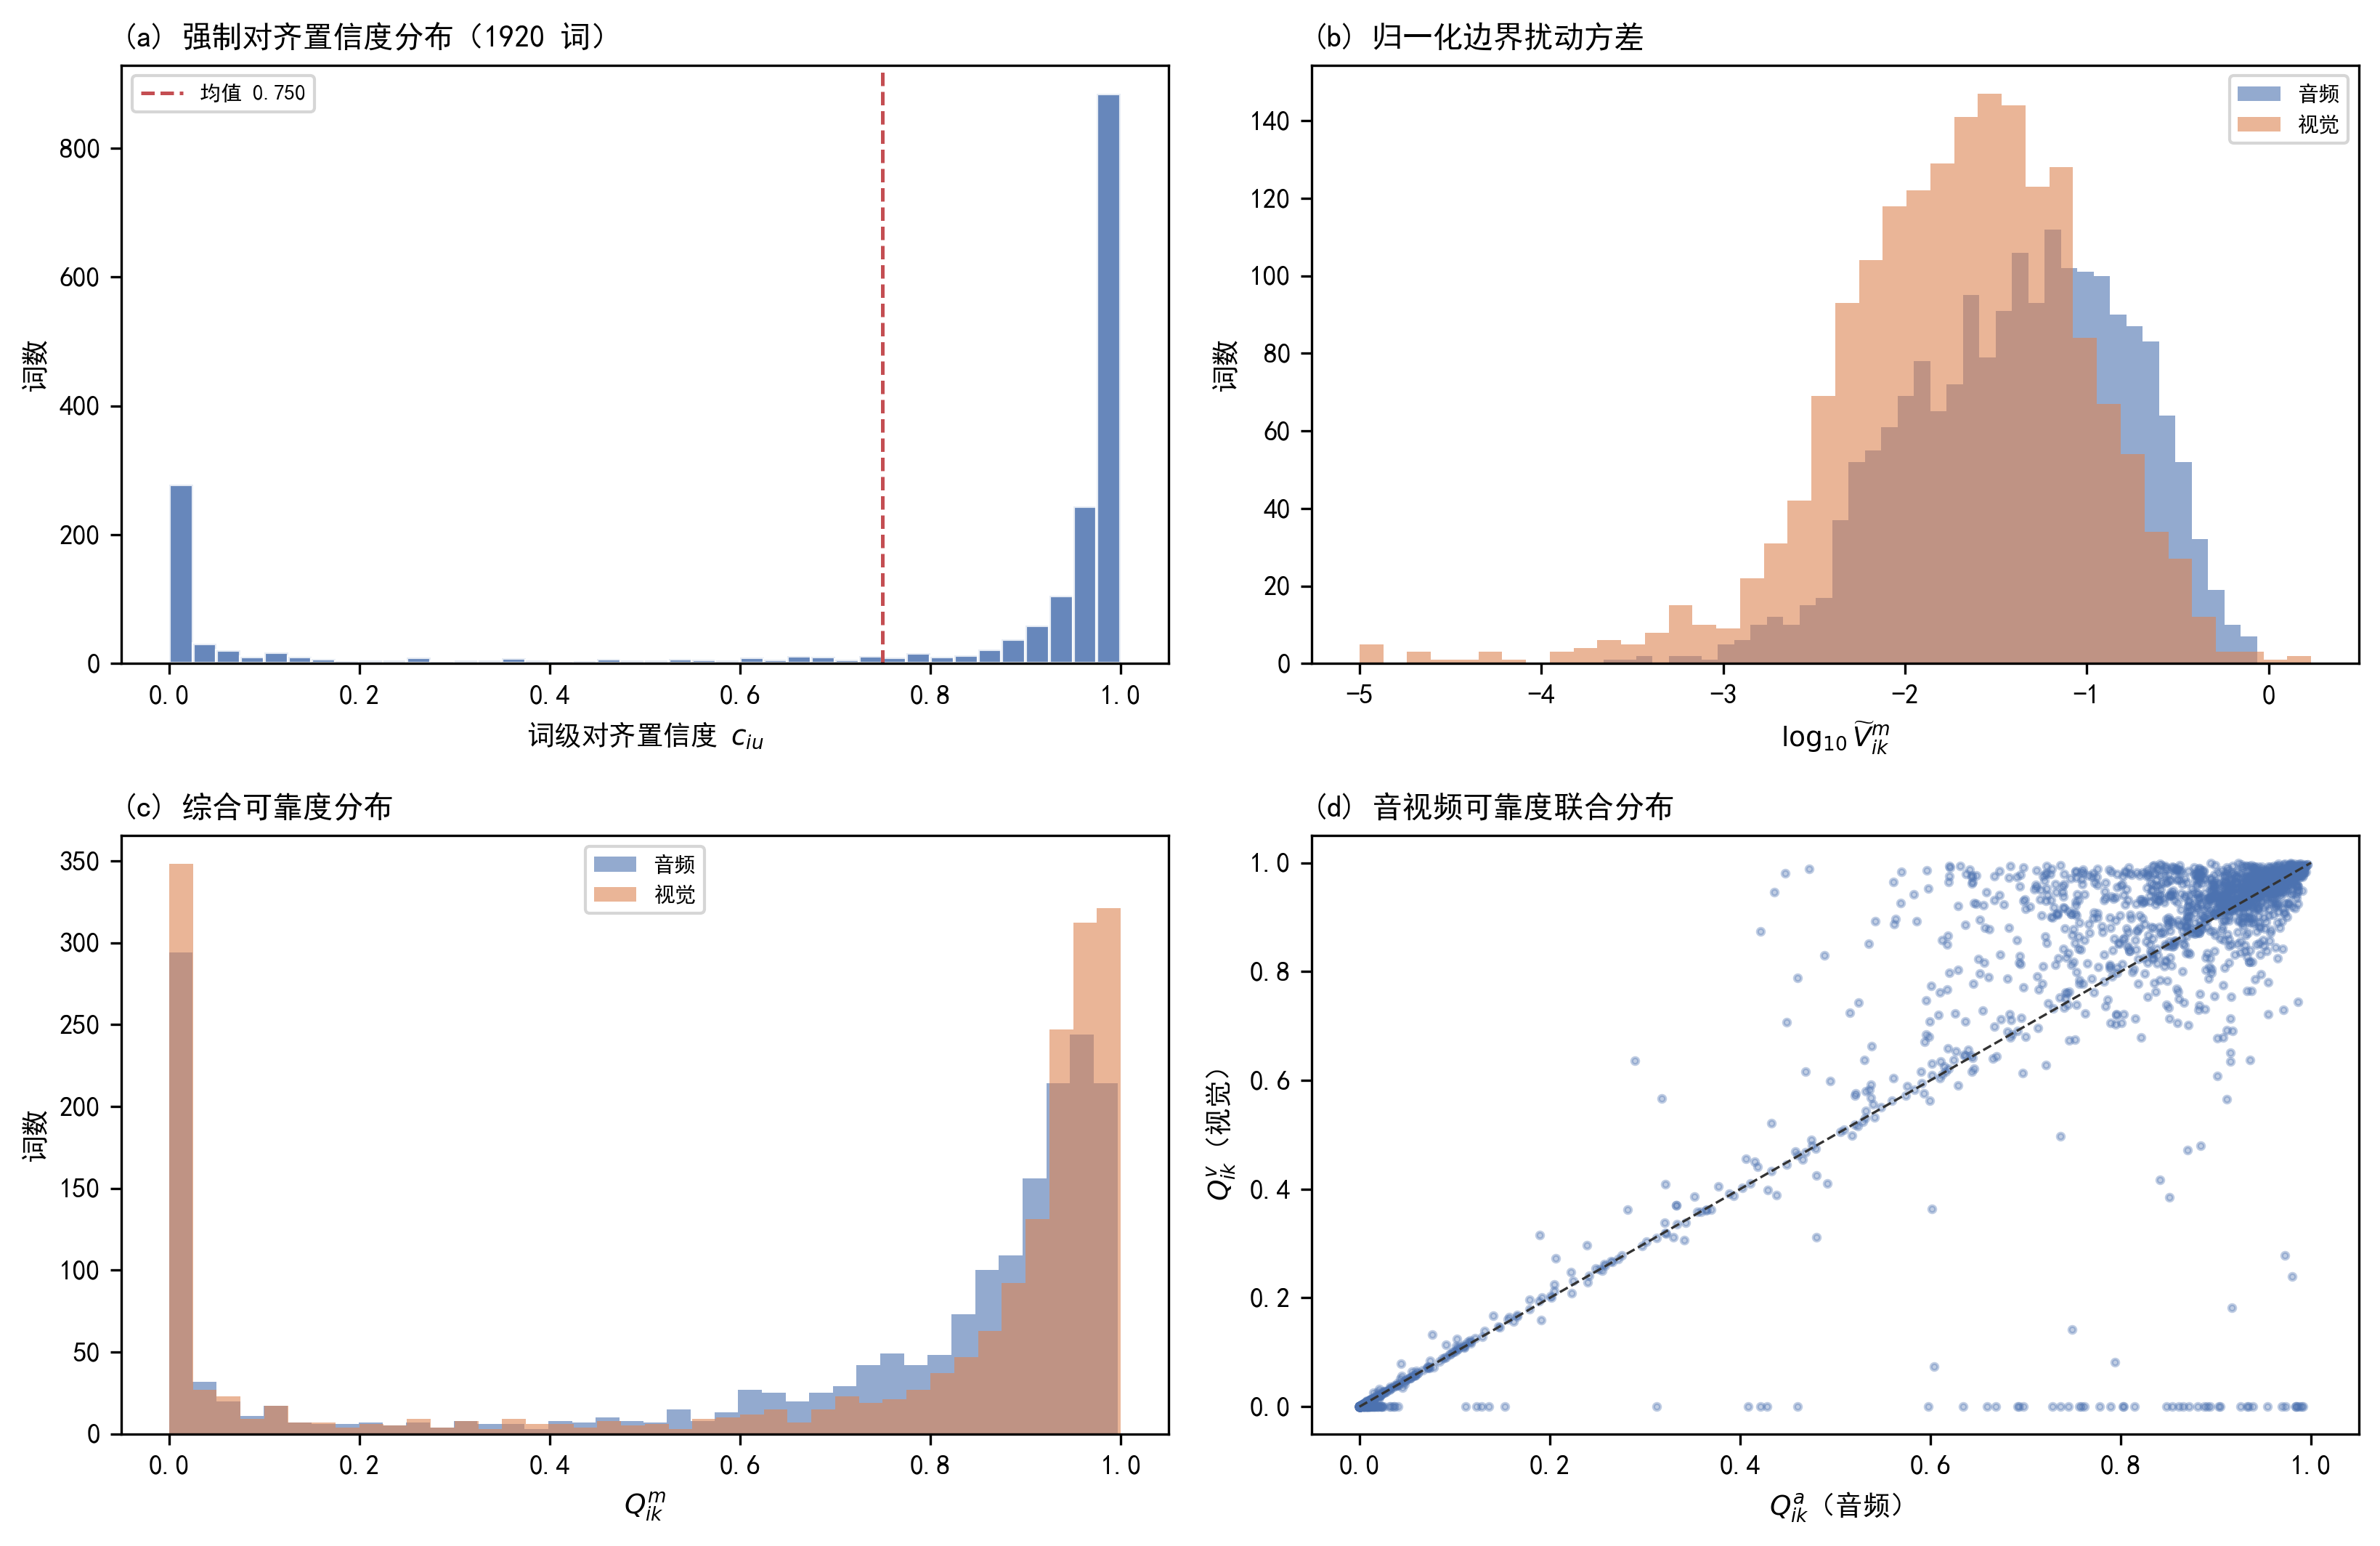
\includegraphics[width=\linewidth]{figures/q1_quality.png}
\caption{1920个已生成词区间的路径置信度、归一化边界扰动方差和综合质量分布}
\label{q1:fig:quality}
\end{figure}

质量分数的三个参数按词区间的时间尺度与模块规模设定：衰减系数$\gamma$控制覆盖偏离的惩罚强度，扰动次数$B$与尺度$s$共同决定边界敏感性的估计精度。表\ref{q1:tab:sensitivity}给出三者变化时的排序一致性，用于检验锚点质量排序是否依赖具体参数设定。

\begin{table}[htbp]
\centering\small
\caption{参数敏感性结果与适用范围}
\label{q1:tab:sensitivity}
\begin{tabularx}{\linewidth}{p{2.1cm}p{4.8cm}Y}
\toprule
实验 & 排序一致性 & 说明 \\
\midrule
$\gamma$变化 & 音频 $Q$：0.5和2相对1的样本内排序相关均值0.974、0.972 & 音频质量分量的排序在该参数取值范围内保持稳定 \\
$B$变化 & 视觉 $V$：50相对200的排序相关0.995 & 在排序前12条样本各前8词上核算的视觉方差排序 \\
$s$变化 & 相对40\,ms，20\,ms的样本内 $Q$ 排序相关均值0.915/0.937，80\,ms为0.960/0.901 & 音频与视觉分别计算的样本内排序一致性 \\
\bottomrule
\end{tabularx}
\end{table}

三项参数的排序一致性均在0.90以上（表\ref{q1:tab:sensitivity}）：参数变化只改变方差与质量的点值，不改变锚点之间的相对次序。相对质量比较因此取$B=50$，$Q$与$V$用于排序与复核抽样，不引用其点值。

\paragraph{时间对齐准确性与时序一致性验证}

时间对齐的验证从有效性、稳健性与一致性三个层面展开：有效性由词界与声学段落的对照及区间结构约束给出，稳健性由边界扰动对特征聚合的影响刻画，一致性由人为错位后的跨模态关联变化检验。

\textbf{（1）边界位置核验。} 以10\,ms步长的RMS包络（25\,ms窗）检测低能量停顿段，阈值取包络95分位的6\%、最短60\,ms，在词界$\pm250$\,ms邻域内度量边界与停顿段的距离，并以词内随机时刻作对照。邻近存在停顿的词界中，39.2\%落在停顿段50\,ms以内，同口径的随机对照为19.5\%，词界落在声学停顿附近的比例约为随机位置的两倍，起点一侧高于终点一侧，词界落在有声段落的交界附近而非与语音段落脱节。区间结构方面，1920个已生成区间在起点非负、长度为正、终点落在音轨有效时长之内与起点随词序单调四项约束上均无违例，词界没有越出所属词序或超出音轨范围。

\textbf{（2）边界扰动实验。} 边界扰动改变池化权重与质量分量，其影响以排序一致性衡量：扰动次数与扰动尺度的变化只改变数值估计，不改变锚点之间的相对次序与相对质量判断（表\ref{q1:tab:sensitivity}），锚点的时间支撑对边界估计误差保持稳健。

\textbf{（3）模态错位实验。} 时间映射的正确性可由错位后的关联下降来检验：若词级对应成立，人为破坏对应关系应使音视频之间的词级关联减弱。据此设计单模态错位实验，保持一侧词窗口不动，仅将另一侧平移$\pm0.25$、$\pm0.5$或$\pm1.0$\,s，比较响度与嘴部开合、嘴部运动的词级相关，共得到12种非零错位条件。所有条件的平均相关均低于各自的样本配对基线，24项Wilcoxon检验中20项在未校正的5\%水平上显著，最小$p$约为$6.8\times10^{-8}$。

在该口径下，任一非零错位都使两项相关下降，且多数差异在统计上显著，表明当前时间映射保持了音视频之间的词级关联，最小错位幅度0.25\,s已足以被该检验分辨。

在人脸检出率较高的样本上，包络相关最大值对应的延迟中位数均为正且不超过0.3\,s，与词区间时长的中位数处于同一时间尺度，说明音频包络与视觉动作在词级窗口内基本对齐。该量记为包络最佳延迟，用于描述词级音视频的联动强度。边界位置核验与错位实验分别从有效性与一致性两端评价时间锚点：词界落在声学停顿附近的比例约为随机位置的两倍，人为破坏时间对应使跨模态词级关联显著减弱，所构造的词级时间锚点与有声段落交界及音视频之间的局部时序对应关系保持一致。

\paragraph{全量样本结果}
表\ref{q1:tab:all100}逐条汇总100条样本。视、音时长采用编辑列表的有效呈现口径，合计分别为\VideoDuration\,s和\AudioDuration\,s；对齐粒度均为原词锚点与子词继承。

T、A、V表示文本、语音和人脸视觉分支；V后的星号、空心圆分别表示部分帧、全片未检出人脸。“区间/词”分母含未对齐项，“内容位”为进入50位接口的内容词元数，上限为48。

\begingroup
\fontsize{8.5}{10.4}\selectfont
\setlength{\tabcolsep}{3pt}
\renewcommand{\arraystretch}{1.02}
\begin{longtable}{rllccrrr}
\caption{附件1全部100条样本的特征提取结果}\label{q1:tab:all100}\\
\toprule
序号 & 样本编号 & 模态 & 视/音时长(s) & T/A/V维度 & 区间/词 & 内容位 & 检出率 \\
\midrule
\endfirsthead
\caption*{续表\ \thetable}\\
\toprule
序号 & 样本编号 & 模态 & 视/音时长(s) & T/A/V维度 & 区间/词 & 内容位 & 检出率 \\
\midrule
\endhead
1 & \texttt{-3g5yACwYnA\$\_\$2} & T+A+V & 9.394/9.231 & 768/25/16 & 14/14 & 17 & 100.0\% \\
2 & \texttt{-3g5yACwYnA\$\_\$3} & T+A+V & 14.389/14.328 & 768/25/16 & 29/29 & 40 & 100.0\% \\
3 & \texttt{-3g5yACwYnA\$\_\$9} & T+A+V & 8.817/8.696 & 768/25/16 & 21/21 & 28 & 100.0\% \\
4 & \texttt{-3g5yACwYnA\$\_\$13} & T+A+V & 5.514/5.399 & 768/25/16 & 15/15 & 18 & 100.0\% \\
5 & \texttt{-3nNcZdcdvU\$\_\$5} & T+A+V$^{*}$ & 7.868/7.788 & 768/25/16 & 18/18 & 22 & 99.6\% \\
6 & \texttt{-571d8cVauQ\$\_\$0} & T+A+V$^{*}$ & 5.167/4.992 & 768/25/16 & 12/12 & 16 & 96.7\% \\
7 & \texttt{-571d8cVauQ\$\_\$5} & T+A+V & 15.273/15.115 & 768/25/16 & 43/43 & 48 & 100.0\% \\
8 & \texttt{-6rXp3zJ3kc\$\_\$8} & T+A+V & 12.805/12.738 & 768/25/16 & 34/34 & 38 & 100.0\% \\
9 & \texttt{-9y-fZ3swSY\$\_\$0} & T+A+V & 6.900/6.757 & 768/25/16 & 22/22 & 28 & 100.0\% \\
10 & \texttt{-9y-fZ3swSY\$\_\$4} & T+A+V & 2.821/2.665 & 768/25/16 & 9/9 & 11 & 100.0\% \\
11 & \texttt{-9y-fZ3swSY\$\_\$8} & T+A+V$^{*}$ & 4.989/4.917 & 768/25/16 & 12/12 & 14 & 91.3\% \\
12 & \texttt{-AUZQgSxyPQ\$\_\$2} & T+A+V & 22.511/22.405 & 768/25/16 & 41/41 & 48 & 100.0\% \\
13 & \texttt{-HeZS2-Prhc\$\_\$2} & T+A+V & 8.262/8.151 & 768/25/16 & 16/16 & 17 & 100.0\% \\
14 & \texttt{-HwX2H8Z4hY\$\_\$2} & T+A+V$^{*}$ & 3.982/3.916 & 768/25/16 & 7/8 & 12 & 23.5\% \\
15 & \texttt{-HwX2H8Z4hY\$\_\$5} & T+A+V$^{*}$ & 5.653/5.544 & 768/25/16 & 9/10 & 10 & 37.5\% \\
16 & \texttt{-HwX2H8Z4hY\$\_\$6} & T+A+V$^{*}$ & 3.358/3.256 & 768/25/16 & 7/7 & 9 & 66.7\% \\
17 & \texttt{-HwX2H8Z4hY\$\_\$9} & T+A+V$^{*}$ & 7.734/7.637 & 768/25/16 & 22/22 & 24 & 12.9\% \\
18 & \texttt{-I\_e4mIh0yE\$\_\$1} & T+A+V & 7.622/7.444 & 768/25/16 & 18/18 & 21 & 100.0\% \\
19 & \texttt{-I\_e4mIh0yE\$\_\$3} & T+A+V & 9.163/8.995 & 768/25/16 & 22/22 & 30 & 100.0\% \\
20 & \texttt{-MeTTeMJBNc\$\_\$0} & T+A+V$^{*}$ & 9.334/9.218 & 768/25/16 & 21/21 & 26 & 99.6\% \\
21 & \texttt{-MeTTeMJBNc\$\_\$7} & T+A+V & 10.517/10.412 & 768/25/16 & 31/31 & 33 & 100.0\% \\
22 & \texttt{-MeTTeMJBNc\$\_\$13} & T+A+V & 5.430/5.255 & 768/25/16 & 14/14 & 16 & 100.0\% \\
23 & \texttt{-NFrJFQijFE\$\_\$1} & T+A+V$^{\circ}$ & 5.746/5.659 & 768/25/16 & 16/16 & 16 & 0.0\% \\
24 & \texttt{-NFrJFQijFE\$\_\$2} & T+A+V$^{\circ}$ & 6.856/6.698 & 768/25/16 & 18/18 & 18 & 0.0\% \\
25 & \texttt{-RfYyzHpjk4\$\_\$2} & T+A+V & 5.516/5.392 & 768/25/16 & 25/25 & 29 & 100.0\% \\
26 & \texttt{-RfYyzHpjk4\$\_\$8} & T+A+V & 4.589/4.532 & 768/25/16 & 17/17 & 21 & 100.0\% \\
27 & \texttt{-RfYyzHpjk4\$\_\$11} & T+A+V & 5.239/5.074 & 768/25/16 & 17/17 & 19 & 100.0\% \\
28 & \texttt{-THoVjtIkeU\$\_\$2} & T+A+V & 4.292/4.230 & 768/25/16 & 10/10 & 11 & 100.0\% \\
29 & \texttt{-THoVjtIkeU\$\_\$6} & T+A+V$^{*}$ & 8.097/7.983 & 768/25/16 & 30/30 & 32 & 99.6\% \\
30 & \texttt{-THoVjtIkeU\$\_\$12} & T+A+V & 14.896/14.805 & 768/25/16 & 39/39 & 42 & 100.0\% \\
31 & \texttt{-UUCSKoHeMA\$\_\$0} & T+A+V$^{*}$ & 7.867/7.732 & 768/25/16 & 18/18 & 23 & 99.6\% \\
32 & \texttt{-UacrmKiTn4\$\_\$4} & T+A+V & 4.741/4.681 & 768/25/16 & 14/14 & 15 & 100.0\% \\
33 & \texttt{-UacrmKiTn4\$\_\$10} & T+A+V & 7.362/7.242 & 768/25/16 & 18/18 & 22 & 100.0\% \\
34 & \texttt{-UuX1xuaiiE\$\_\$0} & T+A+V & 3.700/3.576 & 768/25/16 & 9/9 & 12 & 100.0\% \\
35 & \texttt{-UuX1xuaiiE\$\_\$1} & T+A+V & 10.350/10.267 & 768/25/16 & 27/27 & 33 & 100.0\% \\
36 & \texttt{-UuX1xuaiiE\$\_\$3} & T+A+V & 4.130/4.038 & 768/25/16 & 9/9 & 9 & 100.0\% \\
37 & \texttt{-UuX1xuaiiE\$\_\$6} & T+A+V & 8.114/7.944 & 768/25/16 & 22/22 & 23 & 100.0\% \\
38 & \texttt{-a55Q6RWvTA\$\_\$3} & T+A+V & 22.154/22.084 & 768/25/16 & 65/65 & 48 & 100.0\% \\
39 & \texttt{-aNfi7CP8vM\$\_\$7} & T+A+V & 8.695/8.538 & 768/25/16 & 18/18 & 23 & 100.0\% \\
40 & \texttt{-aqamKhZ1Ec\$\_\$0} & T+A+V & 11.000/10.890 & 768/25/16 & 13/14 & 16 & 100.0\% \\
41 & \texttt{-dxfTGcXJoc\$\_\$0} & T+A+V$^{*}$ & 20.534/20.410 & 768/25/16 & 38/41 & 48 & 78.0\% \\
42 & \texttt{-dxfTGcXJoc\$\_\$1} & T+A+V & 16.161/16.019 & 768/25/16 & 36/36 & 42 & 100.0\% \\
43 & \texttt{-dxfTGcXJoc\$\_\$2} & T+A+V & 16.698/16.633 & 768/25/16 & 32/34 & 40 & 100.0\% \\
44 & \texttt{-dxfTGcXJoc\$\_\$6} & T+A+V & 12.735/12.628 & 768/25/16 & 27/27 & 32 & 100.0\% \\
45 & \texttt{-egA8-b7-3M\$\_\$1} & T+A+V & 10.266/10.156 & 768/25/16 & 19/20 & 22 & 100.0\% \\
46 & \texttt{-egA8-b7-3M\$\_\$6} & T+A+V & 6.265/6.183 & 768/25/16 & 12/12 & 13 & 100.0\% \\
47 & \texttt{-egA8-b7-3M\$\_\$9} & T+A+V & 5.090/4.936 & 768/25/16 & 10/10 & 12 & 100.0\% \\
48 & \texttt{-egA8-b7-3M\$\_\$13} & T+A+V & 4.184/4.024 & 768/25/16 & 11/11 & 16 & 100.0\% \\
49 & \texttt{-egA8-b7-3M\$\_\$16} & T+A+V & 5.538/5.483 & 768/25/16 & 11/11 & 13 & 100.0\% \\
50 & \texttt{-egA8-b7-3M\$\_\$17} & T+A+V & 7.271/7.095 & 768/25/16 & 16/16 & 19 & 100.0\% \\
51 & \texttt{-egA8-b7-3M\$\_\$18} & T+A+V & 8.386/8.266 & 768/25/16 & 22/22 & 27 & 100.0\% \\
52 & \texttt{-egA8-b7-3M\$\_\$20} & T+A+V & 6.645/6.475 & 768/25/16 & 20/20 & 24 & 100.0\% \\
53 & \texttt{-egA8-b7-3M\$\_\$26} & T+A+V & 6.031/5.920 & 768/25/16 & 15/15 & 19 & 100.0\% \\
54 & \texttt{-hnBHBN8p5A\$\_\$6} & T+A+V$^{*}$ & 6.401/6.333 & 768/25/16 & 13/13 & 14 & 82.3\% \\
55 & \texttt{-hnBHBN8p5A\$\_\$7} & T+A+V$^{*}$ & 7.372/7.308 & 768/25/16 & 13/13 & 17 & 60.8\% \\
56 & \texttt{-iRBcNs9oI8\$\_\$3} & T+A+V & 5.621/5.538 & 768/25/16 & 8/8 & 9 & 100.0\% \\
57 & \texttt{-iRBcNs9oI8\$\_\$6} & T+A+V & 2.903/2.821 & 768/25/16 & 5/5 & 5 & 100.0\% \\
58 & \texttt{-iRBcNs9oI8\$\_\$7} & T+A+V & 4.104/4.006 & 768/25/16 & 9/9 & 15 & 100.0\% \\
59 & \texttt{-iRBcNs9oI8\$\_\$8} & T+A+V & 8.093/8.026 & 768/25/16 & 21/21 & 26 & 100.0\% \\
60 & \texttt{-iRBcNs9oI8\$\_\$9} & T+A+V$^{*}$ & 3.416/3.374 & 768/25/16 & 5/5 & 5 & 78.4\% \\
61 & \texttt{-lzEya4AM\_4\$\_\$5} & T+A+V & 7.675/7.570 & 768/25/16 & 19/19 & 21 & 100.0\% \\
62 & \texttt{-lzEya4AM\_4\$\_\$6} & T+A+V & 14.792/14.741 & 768/25/16 & 43/43 & 48 & 100.0\% \\
63 & \texttt{-mJ2ud6oKI8\$\_\$1} & T+A+V$^{\circ}$ & 6.103/6.054 & 768/25/16 & 13/13 & 13 & 0.0\% \\
64 & \texttt{-mJ2ud6oKI8\$\_\$2} & T+A+V$^{*}$ & 5.731/5.702 & 768/25/16 & 11/11 & 17 & 78.4\% \\
65 & \texttt{-mJ2ud6oKI8\$\_\$6} & T+A+V & 2.257/2.229 & 768/25/16 & 5/5 & 5 & 100.0\% \\
66 & \texttt{-mJ2ud6oKI8\$\_\$8} & T+A+V & 4.192/4.172 & 768/25/16 & 11/11 & 11 & 100.0\% \\
67 & \texttt{-mJ2ud6oKI8\$\_\$9} & T+A+V & 7.033/6.909 & 768/25/16 & 22/22 & 29 & 100.0\% \\
68 & \texttt{-mqbVkbCndg\$\_\$0} & T+A+V & 6.500/6.385 & 768/25/16 & 12/12 & 17 & 100.0\% \\
69 & \texttt{-qDkUB0GgYY\$\_\$6} & T+A+V & 4.678/4.614 & 768/25/16 & 16/16 & 18 & 100.0\% \\
70 & \texttt{-ri04Z7vwnc\$\_\$0} & T+A+V$^{\circ}$ & 2.807/2.763 & 768/25/16 & 8/8 & 8 & 0.0\% \\
71 & \texttt{-ri04Z7vwnc\$\_\$2} & T+A+V$^{*}$ & 6.027/5.914 & 768/25/16 & 16/16 & 26 & 35.7\% \\
72 & \texttt{-ri04Z7vwnc\$\_\$5} & T+A+V & 3.545/3.440 & 768/25/16 & 8/9 & 11 & 100.0\% \\
73 & \texttt{-s9qJ7ATP7w\$\_\$0} & T+A+V & 6.867/6.710 & 768/25/16 & 24/24 & 28 & 100.0\% \\
74 & \texttt{-s9qJ7ATP7w\$\_\$1} & T+A+V & 4.792/4.644 & 768/25/16 & 11/11 & 12 & 100.0\% \\
75 & \texttt{-s9qJ7ATP7w\$\_\$4} & T+A+V$^{*}$ & 4.427/4.247 & 768/25/16 & 9/9 & 10 & 71.3\% \\
76 & \texttt{-s9qJ7ATP7w\$\_\$5} & T+A+V & 8.561/8.398 & 768/25/16 & 19/19 & 20 & 100.0\% \\
77 & \texttt{-s9qJ7ATP7w\$\_\$6} & T+A+V$^{*}$ & 2.475/2.315 & 768/25/16 & 5/5 & 5 & 81.7\% \\
78 & \texttt{-s9qJ7ATP7w\$\_\$7} & T+A+V$^{*}$ & 6.966/6.839 & 768/25/16 & 28/28 & 38 & 63.3\% \\
79 & \texttt{-s9qJ7ATP7w\$\_\$8} & T+A+V & 3.295/3.184 & 768/25/16 & 12/13 & 17 & 100.0\% \\
80 & \texttt{-t217m2on-s\$\_\$2} & T+A+V & 5.686/5.630 & 768/25/16 & 12/12 & 16 & 100.0\% \\
81 & \texttt{-t217m2on-s\$\_\$7} & T+A+V & 17.183/17.026 & 768/25/16 & 45/45 & 48 & 100.0\% \\
82 & \texttt{-tANM6ETl\_M\$\_\$3} & T+A+V & 6.758/6.604 & 768/25/16 & 22/22 & 29 & 100.0\% \\
83 & \texttt{-tPCytz4rww\$\_\$10} & T+A+V & 4.789/4.678 & 768/25/16 & 12/12 & 15 & 100.0\% \\
84 & \texttt{-tPCytz4rww\$\_\$11} & T+A+V & 5.467/5.378 & 768/25/16 & 17/17 & 20 & 100.0\% \\
85 & \texttt{-tPCytz4rww\$\_\$12} & T+A+V & 11.864/11.736 & 768/25/16 & 26/26 & 28 & 100.0\% \\
86 & \texttt{-tPCytz4rww\$\_\$16} & T+A+V & 7.206/7.139 & 768/25/16 & 16/16 & 17 & 100.0\% \\
87 & \texttt{-tPCytz4rww\$\_\$18} & T+A+V & 6.645/6.569 & 768/25/16 & 16/16 & 22 & 100.0\% \\
88 & \texttt{-uywlfIYOS8\$\_\$4} & T+A+V & 6.045/5.882 & 768/25/16 & 18/18 & 22 & 100.0\% \\
89 & \texttt{-vxjVxOeScU\$\_\$4} & T+A+V & 9.127/9.037 & 768/25/16 & 21/21 & 27 & 100.0\% \\
90 & \texttt{-wMB\_hJL-3o\$\_\$7} & T+A+V$^{*}$ & 6.044/5.976 & 768/25/16 & 22/22 & 23 & 96.7\% \\
91 & \texttt{-wny0OAz3g8\$\_\$0} & T+A+V & 3.334/3.274 & 768/25/16 & 9/9 & 11 & 100.0\% \\
92 & \texttt{-wny0OAz3g8\$\_\$1} & T+A+V & 6.844/6.776 & 768/25/16 & 22/23 & 28 & 100.0\% \\
93 & \texttt{-wny0OAz3g8\$\_\$2} & T+A+V & 6.687/6.523 & 768/25/16 & 23/23 & 28 & 100.0\% \\
94 & \texttt{-wny0OAz3g8\$\_\$3} & T+A+V & 6.146/6.100 & 768/25/16 & 20/20 & 20 & 100.0\% \\
95 & \texttt{-wny0OAz3g8\$\_\$5} & T+A+V & 6.912/6.741 & 768/25/16 & 20/20 & 27 & 100.0\% \\
96 & \texttt{-wny0OAz3g8\$\_\$7} & T+A+V & 8.068/7.911 & 768/25/16 & 29/29 & 31 & 100.0\% \\
97 & \texttt{-wny0OAz3g8\$\_\$9} & T+A+V & 6.213/6.043 & 768/25/16 & 20/20 & 22 & 100.0\% \\
98 & \texttt{-yRb-Jum7EQ\$\_\$1} & T+A+V & 29.288/29.109 & 768/25/16 & 49/49 & 48 & 100.0\% \\
99 & \texttt{-yRb-Jum7EQ\$\_\$5} & T+A+V & 13.169/13.044 & 768/25/16 & 25/25 & 31 & 100.0\% \\
100 & \texttt{-yRb-Jum7EQ\$\_\$6} & T+A+V & 11.226/11.242 & 768/25/16 & 19/19 & 24 & 100.0\% \\
\bottomrule
\end{longtable}
\endgroup

\FloatBarrier


\FloatBarrier


\subsection{问题二的模型建立与求解}
\label{sec:q2}

\subsubsection{问题分析与建模思路}
问题二使用附件2提供的对齐版三模态特征，训练、验证与测试样本分别为3395、728和727条；附件3提供30条无标签样本，用于局部缺失条件下的专项推理检验。按赛题定义，模态局部缺失指文本、语音或视觉中某一模态的连续若干位置取值全部为零，并不表示整条模态不存在。本问需在局部信息不完整的条件下同时输出情感极性与连续情感强度，并给出缺失模态类型、缺失率、缺失位置与缺口长度对预测性能的影响规律。

三类模态的缺失形式各不相同：文本缺失由词元标记识别，语音与视觉缺失由全零向量识别，三路观测需分别判定；缺口连续分布并横跨多个锚点，以常量填充会把填充值当作观测，直接丢弃受损位置则使信息损失随缺口长度扩大。附件3的缺失在同一时段上跨模态重合，缺口处的三路证据同时弱化，难以依靠单模态冗余补偿。更关键的是补全结果本身可能不可靠：由样本内可用节点估计的替代表示，其质量取决于缺口周围的上下文，本文认为不应与真实观测同等对待。此外，自然缺失的分布由采集过程决定，仅按自然缺失训练难以覆盖各类缺口形态，且类别分布不平衡，需要配合受控遮挡与类别平衡处理。

据此，本文采用以三态状态区分观测与缺损、以可靠度控制补全参与度的建模方案，构造三态感知可靠补全与融合网络TSRF-D。有效观测、结构填充与局部缺失三种状态随输入一并进入模型；缺损位置由样本内可用节点检索生成补全表示，可靠度门控决定其与回退表示的融合比例，再经双向时序编码与双任务头输出极性概率与连续强度。训练以EMT-DLFR\cite{ref:emt}作为异构教师：教师在原始可用输入上产生软目标并保持冻结，学生在局部缺失输入下同时接受类别平衡的真实标签监督、任务蒸馏以及补全与门控的辅助监督。三类信号分工不同：教师保留判别能力，补全分支处理表示缺口，门控判断补全是否可信。总体结构如图\ref{q2:fig:arch}所示。

模型在50个对齐位置上统一输出极性与强度；模型评价从基础性能、缺失条件（模态类型、缺失率、位置与缺口长度）、输入模态消融与基线对照以及附件3全量推理四个方面展开，全部使用同一特征版本与同一输入接口。

\subsubsection{数据准备}
\paragraph{数据划分与输入接口}
附件2提供4850条样本，按题目给定划分使用3395条训练样本、728条验证样本和727条测试样本；附件3为30条无标签样本，仅参与专项预测，其输出以全量预测与预测概率分布的形式汇总。两批数据均采用对齐版本：附件2为\file{aligned\_50}，每个样本至多50个对齐位置；附件3为对齐版本目录下的同名样本，字段组织与张量形状与附件2一致。输入张量分别为$X^t\in\R^{50\times768}$、$X^a\in\R^{50\times74}$、$X^v\in\R^{50\times35}$。三分类标签依次对应负向、中性和正向，其中0仅属于中性类；训练集三类样本数依次为967、758和1670，正向样本约占一半，类别分布并不均衡。连续强度标签位于$[-3,3]$，取值包含非整数值，因此按连续回归处理。

为统一训练与专项推理的文本输入，采用冻结的\file{bert-base-uncased}第12层，由\file{text\_bert}中的词元编号、注意力掩码和分段编号重算连续表示。重算特征与附件2自带文本特征的平均绝对偏差约为$6.6\times10^{-7}$，最小余弦相似度约为0.9999997，二者数值一致。由于文本遮挡需要在编码前替换词元，保留词元编号并据此重算，可使遮挡条件正确作用于上下文表示。

三模态特征在同一组对齐锚点上组织，同一锚点的文本、语音与视觉向量视为同一时段的观测；语音与视觉向量按锚点整体给出，模型不再细分锚点内部的帧。所采用的对齐版本中，同一序列位置的三个模态共享官方给定的时间对应关系，局部缺失的长度以锚点数度量；本问与问题三因此只处理各位置的观测可用性，不再重新估计时间对应关系。

\paragraph{缺失分布与缺口形态}
附件2的自然缺失在各模态间并不均衡：视觉缺失约占内容位的5.5\%，分布在421条样本中，缺口平均跨越7.5个锚点、最长48个；音频缺失约占0.08\%，仅见于4条样本；文本不含缺失标记。附件3为赛题构造的模态缺失样本，文本、语音和视觉分别缺失131、131和135个内容位，合计95段，其中71段长度为1，平均每条样本3.17段；其文本与语音的缺失位置在全部30条样本上逐位重合，文本与视觉在29条样本上重合，缺失呈多模态局部同段共缺的形态，另有3条样本不含缺失。两批数据的缺口均以连续段而非孤立点的形式跨越若干锚点，因此遮挡实验的缺口以连续区间为基本单位构造。

\paragraph{内容、观测与人工缺失掩码}
记样本为$i$，锚点为$k$，模态$m\in\{t,a,v\}$。内容掩码$P_{ik}$由注意力有效位排除\file{[CLS]}和\file{[SEP]}得到。自然观测掩码分别定义为
\begin{align}
 O^t_{ik}&=P_{ik}\ind\{\mathrm{token}_{ik}\ne[\mathrm{UNK}]\},\\
 O^a_{ik}&=P_{ik}\ind\{X^a_{ik}\ne\bm0\},\qquad
 O^v_{ik}=P_{ik}\ind\{X^v_{ik}\ne\bm0\}.
\end{align}
其中$X^m_{ik}\ne\bm0$表示该向量至少有一个非零分量。全零向量与文本\file{[UNK]}表示该位置观测不可用，而不是有效的特征取值：零值本身不携带情感信息，缺失由掩码表达而不由取值表达，填充、观测与局部缺失三种状态由此唯一确定。

令人工遮挡掩码为$H^m_{ik}$，且$H^m_{ik}\le O^m_{ik}$，则最终观测掩码$\widetilde O^m_{ik}=O^m_{ik}(1-H^m_{ik})$。三态变量定义为
\begin{equation}
s^m_{ik}=\begin{cases}
0,&P_{ik}=0,\\1,&P_{ik}=1,\ \widetilde O^m_{ik}=1,\\2,&P_{ik}=1,\ \widetilde O^m_{ik}=0.
\end{cases}
\end{equation}
自然缺失与人工缺失在模型输入中均为状态2，但仅人工遮挡位置保留可用于重建评价的原始真值。对模态$m$的第$j$维，使用训练集观测位置估计$\mu^m_j,\sigma^m_j$并计算
\begin{equation}
\bar X^m_{ikj}=\frac{X^m_{ikj}-\mu^m_j}{\widetilde\sigma^m_j},\qquad
\widetilde\sigma^m_j=\begin{cases}1,&\sigma^m_j<10^{-6},\\\sigma^m_j,&\text{其他}.
\end{cases}
\end{equation}
结构位在标准化后置零，缺失位通过观测掩码排除于候选集合之外。人工音视频遮挡使用标准化空间中的零值；文本则先将选定词元替换为\file{[UNK]，再经BERT编码}，同时保留原有序列位置，使未遮挡位置的上下文表示不含已删除词元的信息。

\subsubsection{模型构建}
\paragraph{总体结构与三态投影}
图\ref{q2:fig:arch}给出学生网络及教师监督的关系。学生的计算顺序为投影、补全与门控、时序编码、池化和双任务预测：三态投影先给出区分位置的节点表示，补全分支在样本内检索有效观测，为缺失位生成替代表示，门控决定其参与比例，随后由时序编码与池化得到样本级表示。补全位于时序编码之前，使递归编码面对的是完整序列，缺口通过检索结果而不是零值进入后续计算。
\begin{figure}[htbp]\centering
\begin{tikzpicture}[font=\small,
 box/.style={draw=black!65,fill=black!3,text width=9.9cm,align=center,minimum height=9mm,inner sep=4pt},
 arr/.style={-{Latex[length=2mm]},thick}]
\node[box] (x) {缺失输入：词元先遮挡再编码；音视频连续锚点遮挡};
\node[box,below=4mm of x] (p) {模态投影 + 位置、模态和三态嵌入};
\node[box,below=4mm of p] (c) {样本内观测节点检索补全 + 可靠度门控融合};
\node[box,below=4mm of c] (g) {逐模态BiGRU + 内容位均值/最大池化 + 可用比例};
\node[box,below=4mm of g] (h) {共享MLP：三分类概率 $p^S$ 与连续强度 $\hat r^S$};
\node[box,below=6mm of h] (t) {冻结EMT-DLFR教师：原始可用输入 $\to (p^T,\hat r^T)$\\类别平衡标签监督 + 任务蒸馏 + 重建与门控辅助监督};
\draw[arr] (x)--(p);\draw[arr] (p)--(c);\draw[arr] (c)--(g);\draw[arr] (g)--(h);
\draw[arr,dashed] (t)--node[right,font=\footnotesize]{训练期监督}(h);
\end{tikzpicture}
\caption{TSRF-D网络结构与教师--学生监督关系}\label{q2:fig:arch}
\end{figure}

将三模态特征映射到公共维度$d=64$。设模型实际接收的标准化输入为$\widetilde x^m_{ik}$，则
\begin{equation}
z^m_{ik}=P_{ik}\left(W_m\widetilde x^m_{ik}+b_m+
e_m^{\mathrm{mod}}+e_{s^m_{ik}}^{\mathrm{state}}+e_k^{\mathrm{pos}}\right).
\end{equation}
模态嵌入描述信息来源，状态嵌入表征可观测性，位置嵌入保留序列顺序，三者共同形成缺失感知的节点表示。三个模态经各自的仿射映射进入同一$d=64$维空间，使补全检索可以在跨模态候选之间比较表示距离；结构位在投影后置零，不参与检索与池化。

\paragraph{观测节点加权补全}
对样本$i$，以$\Omega_i=\{(n,j):\widetilde O^n_{ij}=1\}$为候选集。缺失位置的查询及候选键值为
\begin{equation}
q^m_{ik}=Q(e_k^{\mathrm{pos}}+e_m^{\mathrm{mod}}+e_2^{\mathrm{state}}),\quad
\kappa^n_{ij}=K_z(z^n_{ij}),\quad v^n_{ij}=V_z(z^n_{ij}),
\end{equation}
其中$Q,K_z,V_z$为可学习仿射映射。缺失位置没有自身观测，其表示只能由样本内其他有效节点估计；查询由目标位置、模态与缺失状态（$s^m_{ik}=2$）共同确定，不包含目标位的内容信息，候选键值由有效观测生成，从而把待补位置的结构信息与候选节点的样本内容分开处理。

设$\ell^n_{ij}$为候选位置所在连续观测段的长度，定义观测连续性先验
\begin{equation}
u^n_{ij}=\sigma\left(\alpha_0+\alpha_1\widetilde O^n_{ij}
+\alpha_2\min(\ell^n_{ij}/10,1)\right).
\end{equation}
该先验利用连续观测段长度描述候选节点的局部可用性：位于较长连续观测段上的候选更贴近缺口的上下文，孤立观测的参考价值较低。对$(n,j)\in\Omega_i$，补全代价及权重为
\begin{align}
C^{m,n}_{i,k,j}&=\frac{\|q^m_{ik}-\kappa^n_{ij}\|_2^2}{d}
+\lambda_t\frac{|k-j|}{K}+\lambda_q(1-u^n_{ij}),\\
\pi^{m,n}_{i,k,j}&=\frac{\exp(-C^{m,n}_{i,k,j}/\tau)}
{\sum_{(n',j')\in\Omega_i}\exp(-C^{m,n'}_{i,k,j'}/\tau)},\qquad
\hat z^m_{ik}=\sum_{(n,j)\in\Omega_i}\pi^{m,n}_{i,k,j}v^n_{ij}.
\end{align}
上述代价综合表示距离、位置距离和观测连续性，其中位置距离以接口长度$K$归一，时间项赋予邻近锚点较高的候选优先级，连续性项抑制孤立观测的权重；温度$\tau$控制权重在候选间的集中程度，取值较小时结果接近最近候选，取值较大时趋于候选均值。候选范围覆盖样本内全部可用模态，因而兼顾同模态时序信息与跨模态关联信息。

\paragraph{可靠度门控与情感预测}
对候选代价按补全权重聚合，得到门控所需的三个统计量：
\begin{equation}
\begin{aligned}
\overline C^{m}_{ik}&=\sum_{(n,j)\in\Omega_i}\pi^{m,n}_{i,k,j}C^{m,n}_{i,k,j},\qquad
C_{\min}=\min_{(n,j)\in\Omega_i}C^{m,n}_{i,k,j},\\
\operatorname{Var}_{\pi}(C)&=\sum_{(n,j)\in\Omega_i}\pi^{m,n}_{i,k,j}\left(C^{m,n}_{i,k,j}-\overline C^{m}_{ik}\right)^2.
\end{aligned}
\end{equation}
以三者与候选数量占比、目标模态可用比例构造门控输入
\begin{equation}
g^m_{ik}=\left[\overline C,\operatorname{Var}_{\pi}(C),C_{\min},
|\Omega_i|/(3K),a_i^m,e_m^{\mathrm{mod}}\right],\qquad
a_i^m=\frac{\sum_k\widetilde O^m_{ik}}{\sum_kP_{ik}}.
\end{equation}
两层感知机输出$\rho^m_{ik}=\sigma(G(g^m_{ik}))$，并与可学习的缺失嵌入$e_m^{\mathrm{miss}}$融合：
\begin{equation}
z^{m,f}_{ik}=\widetilde O^m_{ik}z^m_{ik}
+P_{ik}(1-\widetilde O^m_{ik})
\left[\rho^m_{ik}\hat z^m_{ik}+(1-\rho^m_{ik})e_m^{\mathrm{miss}}\right].
\end{equation}
门控输入同时刻画补全的质量与可用证据：加权代价均值与最小代价反映候选的匹配程度，加权方差反映候选之间的分歧，候选数量占比与模态可用比例反映可检索证据与模态自身的完整度。其中$e_m^{\mathrm{miss}}$为模态$m$的可学习缺失嵌入，$\rho^m_{ik}\in(0,1)$由两层感知机给出，调节补全表示对融合结果的贡献。观测位置的表示保持不变，缺失位置在补全与缺失嵌入之间按$\rho$加权；当候选集为空时，令$\pi=0,\rho=0$，以缺失嵌入完成回退。

锚点顺序承载情感的时序演变，因此对每个模态独立进行单层双向GRU编码，记输出隐状态为$h^m_{ik}\in\R^{64}$；缺失位置经融合后已有表示，递归过程面对的是完整序列。实现中按有效前缀打包序列，避免尾部填充通过反向递归污染内容位置。池化只在内容位进行，取内容位的均值与最大值：
\begin{equation}
\bar h^m_i=\frac{\sum_k P_{ik}h^m_{ik}}{\sum_k P_{ik}},\qquad
\check h^m_i=\max_{k:P_{ik}=1}h^m_{ik},\qquad
h_i=\operatorname{MLP}\left(\left[\bar h^t_i,\check h^t_i,\bar h^a_i,\check h^a_i,\bar h^v_i,\check h^v_i,a^t_i,a^a_i,a^v_i\right]\right),
\end{equation}
使结构化填充不参与统计，拼接维度为$6d+3=387$。双任务输出为
\begin{equation}
p_i=\operatorname{softmax}(W_ch_i+b_c),\qquad
\hat y_i=\arg\max_c p_{ic},\qquad
\hat r_i=3\tanh(w_r^\top h_i+b_r).
\end{equation}
分类与回归采用共享表示和独立输出头，强度以$3\tanh(\cdot)$输出，与标签区间$[-3,3]$一致；两个任务通过下文的一致性损失建立软约束。

\paragraph{真实标签与任务蒸馏}
教师采用EMT-DLFR的任务适配结构\cite{ref:emt}。文本经线性投影，语音和视觉经单向LSTM编码到64维；两层、四头的高效多模态Transformer在全局模态表示与局部序列之间交互，融合表示经双任务头输出三类logits和连续强度。教师训练同时使用基础与遮挡输入的标签监督，并结合高层表示吸引和低层特征重建目标；参数仅在附件2训练集上学习，保存轮次由验证集联合指标确定。

教师在同一批样本上使用未追加人工遮挡的输入，其输出反映较完整观测下的情感倾向。教师完成训练后冻结参数，为每个学生种子提供对应教师在训练样本上的输出；学生接收含人工遮挡的输入，通过任务蒸馏\cite{ref:kd}学习教师的类别分布与强度输出，以软目标的形式继承这部分判别信息。蒸馏只在输出层进行，不在隐藏层施加额外对齐约束，以免与补全重建、门控监督叠加后各目标相互牵制。学生真实标签监督为
\begin{equation}
\mathcal L_{\mathrm{sup}}=\operatorname{CE}_w(y,p^S)
+\lambda_r\operatorname{Huber}_1(r,\hat r^S)
+\lambda_c\left[(p^S_{+}-p^S_{-})-\tanh(\hat r^S/3)\right]^2,
\end{equation}
其中$p^S_+$与$p^S_-$分别为正、负类别的预测概率，$\lambda_r$与$\lambda_c$为回归项与一致性项权重，$\operatorname{Huber}_\delta$表示$\delta$尺度的Huber损失，$\delta=1$时与$\beta=1$的平滑L1损失一致。设训练集样本量为$N$，类别$c$的样本量为$N_c$，取$w_c=N/(3N_c)$。对训练批次$\mathcal B$，分类损失按实际样本权重归一化：
\begin{equation}
\label{q2:eq:class_weight}
\operatorname{CE}_w(y,p^S)=-\frac{\sum_{i\in\mathcal B}w_{y_i}\log p^S_{i,y_i}}
{\sum_{i\in\mathcal B}w_{y_i}}.
\end{equation}
回归与一致性损失仍按样本平均。类别权重仅作用于真实标签的分类损失，以平衡不同类别对监督目标的贡献；不改变训练采样频率和预测时的最大概率决策规则。教师与学生的分类logits记为$o^T,o^S$，温度为$T$，蒸馏目标为
\begin{align}
\mathcal L_{\mathrm{dc}}&=T^2\operatorname{KL}\left(
\sg[\operatorname{softmax}(o^T/T)]\ \|\ \operatorname{softmax}(o^S/T)\right),\\
\mathcal L_{\mathrm{dr}}&=\operatorname{Huber}_1\left(\hat r^S,\sg[\hat r^T]\right).
\end{align}
$\sg$表示停止梯度。训练采用样本等权的蒸馏损失，并离线缓存教师在训练样本上的输出，使蒸馏不引入在线前向开销。分类蒸馏传递类别间的分布信息，强度蒸馏约束连续预测，两者共同指导学生学习缺失条件下的情感表示。

\paragraph{补全与相对可靠度监督}
对具有真值的人工遮挡集合$\mathcal H_m$，使用可学习解码头$D_m$将补全表示映射回原始标准化特征空间：
\begin{equation}
\mathcal L_{\mathrm{rec}}=\frac{1}{|\mathcal M_H|}\sum_{m\in\mathcal M_H}
\frac{1}{|\mathcal H_m|}\sum_{(i,k)\in\mathcal H_m}
\operatorname{Huber}_1\left(D_m(\hat z^m_{ik}),\bar X^{m,\mathrm{true}}_{ik}\right),
\end{equation}
其中$\bar X^{m,\mathrm{true}}_{ik}$为人工遮挡前的标准化特征，$\mathcal M_H$为当前批次存在人工遮挡的模态集合，每个向量的损失对特征维取均值。重建只在人工遮挡位置计算：这些位置同时具备缺口输入与被遮挡前的真值，自然缺失位置没有可比的原始观测。重建目标为标准化后的原始特征，解码头与学生网络共同训练。

补全表示与回退表示经同一解码头映射回特征空间，二者相对真值的逐位置平均绝对误差为
\begin{equation}
\begin{aligned}
e_{\mathrm{rec}}&=\frac{1}{|\mathcal H_m|}\sum_{(i,k)\in\mathcal H_m}\frac{1}{d}\left\|D_m(\hat z^m_{ik})-\bar X^{m,\mathrm{true}}_{ik}\right\|_1,\\
e_{\mathrm{fal}}&=\frac{1}{|\mathcal H_m|}\sum_{(i,k)\in\mathcal H_m}\frac{1}{d}\left\|D_m(e_m^{\mathrm{miss}})-\bar X^{m,\mathrm{true}}_{ik}\right\|_1,
\end{aligned}
\end{equation}
据此构造门控监督目标
\begin{equation}
\rho^*=\sg\left[\sigma\left((e_{\mathrm{fal}}-e_{\mathrm{rec}})/\tau_{\rho}\right)\right],\qquad
\mathcal L_{\mathrm{rel}}=\operatorname{BCE}(\rho,\rho^*).
\end{equation}
可靠度损失同样先在各模态人工遮挡位平均，再在有遮挡模态间平均。该目标以补全与回退的相对误差为标签，使门控判断补全是否优于回退，而不依赖误差绝对水平的标定。自然缺失位置没有可用真值，不参与上述两项监督，其门控取值由这些监督训练得到的映射外推给出。

综合目标为
\begin{equation}
\label{q2:eq:total_loss}
\mathcal L=\mathcal L_{\mathrm{sup}}+\beta_e\left(
\lambda_{\mathrm{dc}}\mathcal L_{\mathrm{dc}}+
\lambda_{\mathrm{dr}}\mathcal L_{\mathrm{dr}}+
\lambda_{\mathrm{rec}}\mathcal L_{\mathrm{rec}}+
\lambda_{\mathrm{rel}}\mathcal L_{\mathrm{rel}}\right).
\end{equation}
首轮$\beta_e=0$，学生先以真实标签建立基础预测能力；随后三轮线性升至1，使补全、门控与蒸馏目标逐步加入，避免辅助目标在训练初期主导优化。预热阶段保留分类、回归和一致性损失。

\subsubsection{模型求解与参数设置}
\paragraph{遮挡策略与训练流程}
附件3的缺失多为局部的连续片段，且可同时落在多个模态上，程度随样本而异。人工缺失若只用单一形态生成，模型容易被固定模式牵着走，因此训练中的遮挡由无新增遮挡、单模态局部缺口、多模态缺失与整模态丢弃四类场景混合而成，采样比例依次为20\%、45\%、25\%与10\%。占比最高的单模态局部缺口对应附件3的主要形态；多模态缺失描述跨模态证据同时衰减，其中三模态组合按各模态独立的位置生成缺口，使缺口部分交叠而非整齐重合；整模态丢弃把所选模态的内容位全部抹去，观测缺失达到极端，仅以10\%的比例作为压力场景；无新增遮挡保留自然缺失，使模型在训练全程都能接触未追加遮挡的样本，基础判别能力不随缺失场景占比上升而退化。

单模态缺口的比例围绕附件3的实际缺失水平展开：文本给出10\%、25\%与40\%三档，把附件3的水平包在中间，语音与视觉固定取20\%，与附件3两路约两成的缺失程度相当。文本的分档更细，因为极性判断对文本证据的依赖最强，同等比例下文本损失对判别的影响也最直接。多模态缺失覆盖双模态与三模态组合，比例取15\%至30\%。

所有人工遮挡都嵌套在自然观测之内，即$H^m\le O^m$，只改变原本可观测内容位的取值，自然缺失与人工缺失在掩码上始终可区分。生成方式按代价分开处理：文本遮挡必须在编码前替换词元，逐轮重算上下文的开销过高，因此含文本的9类遮挡模式按样本预生成编码结果，在轮次间轮换；语音与视觉直接在特征位图上置零，不含文本的模式按种子与轮次在线生成，同一随机流下课程可复现。

局部缺口的段长由参数0.35的几何分布采样，短缺口占多数并保留较长尾部，同时受目标遮挡预算、单段32锚点的长度上界与样本边界约束：预算只规定该样本的遮挡总量，缺口按预算逐段铺开，触及样本末端即截断。按最终掩码统计，局部与多模态场景中的遮挡平均覆盖约10\%的内容锚点，段长以1至4个锚点为主，与附件3以短缺口为主的形态同向；训练中保留的较长缺口，使评测中加长缺口的条件仍落在训练分布附近。

\paragraph{选模准则与关键参数}
模型以验证集联合指标选择训练轮次：
\begin{equation}
\label{q2:eq:sel}
J=0.5F_{\mathrm{base}}+0.5\left(\frac14\sum_{c\in\mathcal C}F_c\right)
-0.1\operatorname{MAE}_{\mathrm{base}},\quad
\mathcal C=\{t,a,v,tav\}\text{的居中8锚点缺口}.
\end{equation}
其中$F$为Macro-F1，基础项与强度项均在保留自然缺失、不追加人工遮挡的输入上计算。基础性能与缺失性能各占一半权重，强度误差以0.1的系数扣除，使选模同时关注分类与回归：只按基础输入选模会偏向完整观测下的表现，只按缺失条件选模则可能牺牲基础判别能力。选模中的固定8锚点缺口对短样本按有效长度截断，短样本因此出现整段遮挡的压力条件。下文主要评价另以$L_i-1$限制连续区间长度，把选模压力条件与局部缺失评价区分开。教师与学生均按验证集$J$保存参数。

\begin{table}[htbp]\centering\small
\caption{TSRF-D模型与训练参数}\label{q2:tab:params}
\begin{tabularx}{\linewidth}{p{4.4cm}Y}\toprule
参数 & 取值\\\midrule
公共维度、Dropout & 64、0.2\\
时序编码器 & 每模态单层BiGRU；单方向隐维32\\
补全参数 & $\tau=0.5,\lambda_t=0.1,\lambda_q=0.5$\\
观测连续性先验 & $\alpha_0=0,\alpha_1=2,\alpha_2=0.5$；段长尺度10\\
损失权重 & $\lambda_r=1,\lambda_c=0.2,\lambda_{\mathrm{rec}}=0.5,\lambda_{\mathrm{rel}}=0.3$\\
蒸馏与门控目标 & $\lambda_{\mathrm{dc}}=\lambda_{\mathrm{dr}}=1,T=2,\tau_{\rho}=0.2$\\
优化器与调度 & AdamW，初始学习率0.0015，权重衰减$10^{-4}$，余弦调度\\
批量、轮数、早停 & 256、至多32轮、耐心值8；梯度裁剪范数5\\
教师与分类权重 & EMT-DLFR任务适配版；$w_c=N/(3N_c)$，按训练标签计算\\
随机种子与集成 & 教师、学生均使用0、1、2；学生预测概率与强度分别取均值\\
计算环境 & Python 3.12，PyTorch 2.8.0+cu128；RTX 5060 Ti；冻结BERT重算文本\\\bottomrule
\end{tabularx}\end{table}

模型参数由附件2训练集学习，保存轮次由验证集确定。标准化统计量仅由训练集观测位置估计并在后续阶段保持固定，验证集、附件3与附件4沿用同一组统计量，以避免推理阶段引入测试数据的信息，并使跨附件的指标处于同一尺度。

关键参数按以下依据确定。公共维度取$d=64$，在压缩三路高维输入的同时控制参数量，学生网络含约22万参数；补全温度$\tau=0.5$使权重集中在代价较小的候选上；观测连续性先验的段长尺度取10，与常见连续观测的长度量级相当。损失项中真实标签、分类蒸馏与强度蒸馏取同量级权重（$\lambda_r=\lambda_{\mathrm{dc}}=\lambda_{\mathrm{dr}}=1$），重建与门控监督取较小权重（0.5与0.3），使辅助目标不主导优化；一致性项以$\lambda_c=0.2$约束极性与强度的方向一致。优化采用AdamW与余弦学习率调度，初始学习率0.0015、权重衰减$10^{-4}$、梯度裁剪范数5；批量取256，最多训练32轮，验证指标连续8轮无改善即停止并恢复最优参数。三个种子独立训练，预测概率与强度分别取均值集成。在本轮设置下，三个学生种子分别在第7、第8和第22轮取得最优验证指标，训练在第15、16和30轮触发早停，单种子学生训练耗时约40至80\,s。

\paragraph{配置依据与类别平衡}
训练集中正向样本占比为49.19\%，中性样本占比为22.33\%。若对所有样本赋予相同分类权重，正向类别在经验损失中具有更大的总权重。本文采用式\eqref{q2:eq:class_weight}，使各类别满足$N_cw_c=N/3$，从训练目标上均衡三类样本的贡献，与Macro-F1逐类等权评价的出发点相一致。具体频数和权重见表\ref{q2:tab:weights}。
\begin{table}[htbp]\centering\small
\caption{由训练集类别频数确定的分类权重}\label{q2:tab:weights}
\begin{tabular}{lrrr}\toprule
类别 & 样本数$N_c$ & 样本占比/\% & 权重$w_c$\\\midrule
负向 & 967 & 28.48 & 1.1703\\
中性 & 758 & 22.33 & 1.4930\\
正向 & 1670 & 49.19 & 0.6776\\\bottomrule
\end{tabular}\end{table}

权重规则另与温和平衡方案$w_c=[N/(3N_c)]^{1/4}$作过比较：后者在验证集上取得小幅分类增益，但在训练集内部按来源视频分组的两组留出检查中，其局部平均F1相对等权重分别下降0.0123和0.0106，检查覆盖20\%连续缺口的七种模态组合及三个位置。增益未跨划分复现，因此采用由训练频数直接确定的逆频率权重，不再对权重指数作额外搜索。

\paragraph{教师--学生训练算法}
算法\ref{q2:alg:training}给出完整求解步骤，按教师训练、学生训练与集成的顺序展开：每轮重新采样遮挡场景并重建三态变量，损失权重按轮次升温。学生训练同时结合真实标签、蒸馏与重建辅助目标，预生成的文本遮挡特征按相应掩码索引，以保持输入与监督位置的一致性。
\begin{algorithm}[htbp]
\caption{TSRF-D教师--学生联合训练}\label{q2:alg:training}
\small
\textbf{输入：}附件2训练集$\mathcal D_{\mathrm{tr}}$、验证集$\mathcal D_{\mathrm{val}}$，冻结BERT，
缺失场景分布$\mathcal Q$，损失权重，种子集合$\{0,1,2\}$。\par
\textbf{输出：}按验证集联合准则选出的学生参数$\{\theta_S^{*(s)}\}_{s=0}^{2}$。\par
\medskip\noindent
\begin{tabularx}{\linewidth}{@{}r@{\quad}Y@{}}
1 & 构建$P,O$；仅用训练集拟合标准化统计量，由类别频数计算$w_c=N/(3N_c)$，并预生成含文本类的遮挡编码库。\\
2 & \textbf{对每个}随机种子$s\in\{0,1,2\}$，\textbf{执行}：\\
3 & \quad 用训练集学习EMT-DLFR教师，结合基础/遮挡标签监督及双层恢复目标。\\
4 & \quad 按验证集$J$保存教师并冻结；仅缓存训练样本在无新增遮挡输入上的输出。\\
5 & \quad 初始化学生$\theta_S$；令$J^*=-\infty$，最大轮数$E=32$，早停耐心值为8。\\
6 & \quad \textbf{对}$e=1,\ldots,E$，\textbf{执行}：\\
7 & \qquad 依据$\mathcal Q$生成本轮遮挡掩码$H$，限制$H^m\le O^m$，并打乱训练样本。\\
8 & \qquad 设置辅助权重$\beta_1=0$；第2至4轮依次为$1/3,2/3,1$，此后为1。\\
9 & \qquad \textbf{对每个}训练批次$\mathcal B$，\textbf{执行}：\\
10 & \qquad\quad 保留遮挡前标准化真值$\bar X^{\mathrm{true}}$，仅供辅助损失使用。\\
11 & \qquad\quad 将$H^t=1$处词元替换为\file{[UNK]}后编码；按掩码读取预生成文本特征。\\
12 & \qquad\quad 音视频遮挡位使用标准化零值，更新$\widetilde O=O\odot(1-H)$及三态变量。\\
13 & \qquad\quad 学生前向：投影、加权补全、可靠度融合、BiGRU与池化，得到$p^S,\hat r^S$。\\
14 & \qquad\quad 以逆频率类别权重计算$\mathcal L_{\mathrm{sup}}$，读取教师输出$p^T,\hat r^T$。\\
15 & \qquad\quad 计算分类与强度蒸馏损失$\mathcal L_{\mathrm{dc}},\mathcal L_{\mathrm{dr}}$；教师停止梯度。\\
16 & \qquad\quad 仅在人工遮挡位计算$\mathcal L_{\mathrm{rec}},\mathcal L_{\mathrm{rel}}$；可靠度目标停止梯度。\\
17 & \qquad\quad 按式\eqref{q2:eq:total_loss}汇总损失；反向传播、梯度裁剪，使用AdamW更新学生。\\
18 & \qquad \textbf{结束批次循环}；更新余弦学习率。\\
19 & \qquad 在验证集基础输入及$t/a/v/tav$居中8锚点缺口上按式\eqref{q2:eq:sel}计算$J$，评价时不更新模型参数。\\
20 & \qquad 若$J>J^*$，保存学生参数并更新$J^*$；否则连续8轮无改善时提前停止。\\
21 & \quad \textbf{结束轮次循环}，恢复最优学生参数$\theta_S^{*(s)}$。\\
22 & \textbf{结束种子循环}；返回三组学生参数，用于冻结后的概率与强度集成。\\
\end{tabularx}\par
\end{algorithm}

\begin{figure}[htbp]\centering
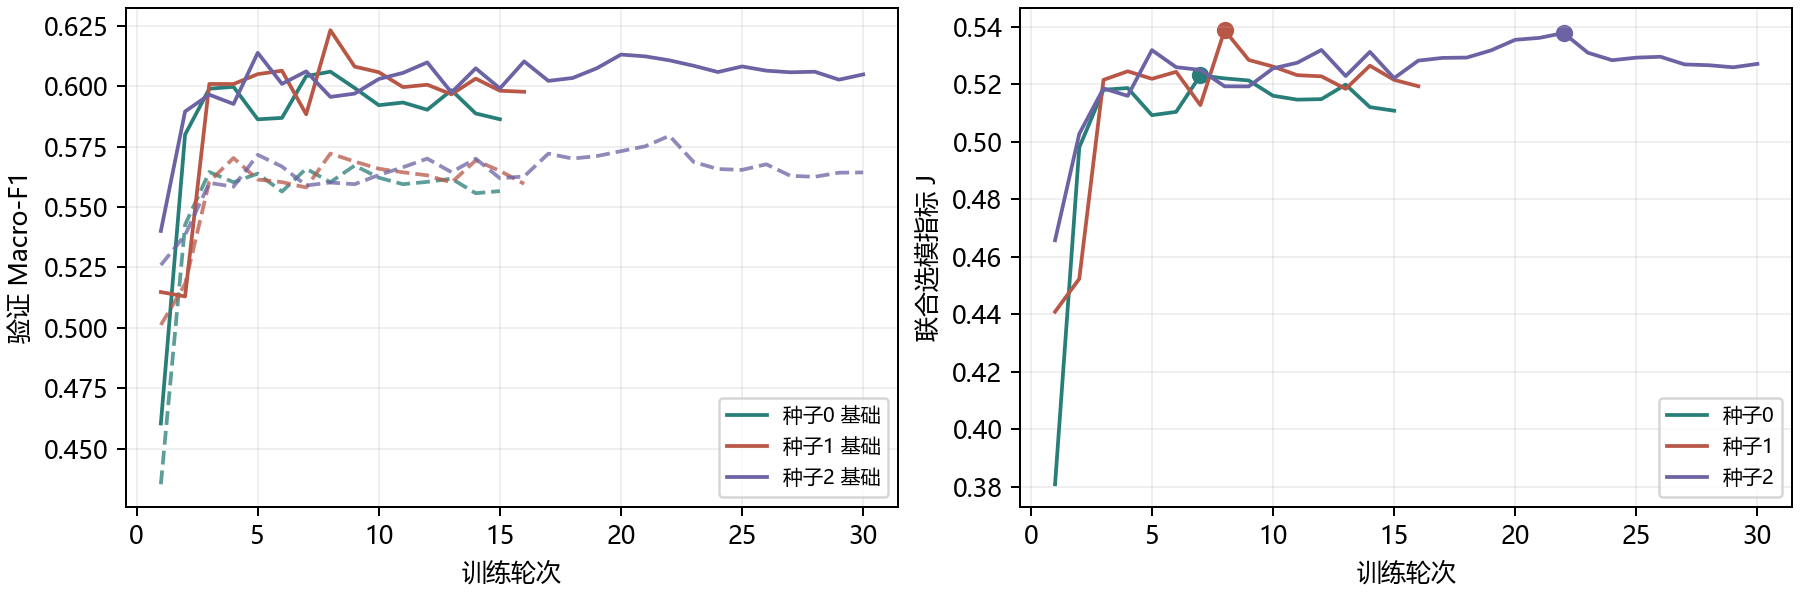
\includegraphics[width=0.9\linewidth]{figures/q2_v4_training.png}
\caption{三个学生种子的训练过程}\label{q2:fig:training}
\end{figure}
如图\ref{q2:fig:training}所示，三个种子的分类指标在训练初期较快上升，随后进入波动区间：每轮的遮挡场景按课程重新采样，场景难度差异会直接反映在验证指标上，因此波动主要来自训练分布的变化，而不是优化过程的不稳定。局部缺失条件下的F1整体低于基础输入，反映出信息遮挡带来的预测损失。联合准则在基础性能与缺失性能之间权衡，保存其最大值对应的学生参数。
\FloatBarrier

\subsubsection{实验结果与分析}

\paragraph{评价协议与基础性能}

评价围绕分类与回归两条线展开。极性是三分类问题，训练集三类样本的比例约为28\%、22\%与49\%，因此以逐类等权的Macro-F1作为主要指标，Accuracy只作为总体正确率的参照；强度是连续量，用MAE衡量误差幅度，用Pearson相关系数衡量预测与标签在排序上的一致程度。三个种子分别独立训练与选模，分类概率与强度输出取均值形成集成结果，以降低初始化差异带来的波动。所有评价都在冻结参数的条件下进行，基础输入保留自然缺失、不追加人工遮挡，作为后面各类缺失干预的共同参照。附件2的有标签测试划分用于性能评价，附件3没有标签，只作专项推理。

冻结参数、不追加人工遮挡时，测试集Macro-F1为0.6189、强度MAE为0.6221，Pearson相关系数为0.6824；验证集在同口径下的结果与之接近，说明选模没有把参数拉向验证集特有的分布。以此为参照，下面依次考察缺失模态、缺失比例、缺口位置与缺口长度四个因素引起的预测变化。

\paragraph{类别权重的求解检验}

类别分布不均会直接影响决策边界：不加权时模型倾向于把边界样本推向样本量大的类别。为观察这一影响，在相同教师、相同学生结构与相同三个种子的条件下，把逆频率权重的结果与等权重学生的验证集预测作对比，两者各自按自身的验证轨迹确定训练轮次。

逆频率加权后，验证集的分类与回归指标变化都落在种子波动的量级之内；分类型看，中性类召回率由0.4891升至0.5978，正向与负向类召回相应回落，预测分布由偏向多数类转向三类相对均衡。本文据此采用由训练频数直接确定的类别权重，并在结果中同时报告总体指标与分类型表现。

\paragraph{连续局部缺失与输入模态消融}

局部缺失的评价在模态组合、缺口比例与缺口位置三个维度上交叉展开，取模态集合$\{t,a,v,ta,tv,av,tav\}$、目标区间比例$\{5\%,10\%,20\%,30\%,40\%\}$以及句首、句中、句尾三个位置，形成105种连续缺失条件。每次干预把所选模态在同一段连续区间内的观测整体移除，对内容长度$L_i\ge2$，区间长度为

\begin{equation}n_i=\min\{L_i-1,\max[1,\lfloor qL_i+0.5\rfloor]\},\quad H^m_{ik}=\ind\{m\in\mathcal M_H,k\in I_i\}O^m_{ik}.\end{equation}

同一段缺口同时落在所选的全部模态上，对应附件3中多路证据在同一时段失效的情形；自然缺失的位置不重复计入人工删除，内容长度不足2的样本不追加遮挡。目标比例以内容锚点为分母，实际新增观测删除率定义为$\sum_{imk}H^m_{ik}/\sum_{imk}O^m_{ik}$，两个量分别保存：未选模态在缺口区间内仍然可用，短样本的区间又会因取整偏离名义比例，目标比例与实现比例并不相等。

按上述规则逐项移除单模态或模态组合的局部信息，构成输入模态消融。表中每种组合对五个比例与三个位置等权平均；全局局部指标对105种条件等权平均，同一视频的不同遮挡版本共用重采样权重，不按独立样本累计，各组合的平均结果见表\ref{q2:tab:local}。

\begin{table}[htbp]\centering\small
\caption{测试集局部输入模态消融结果}\label{q2:tab:local}
\begin{tabular}{lrrr}\toprule
移除的局部模态 & Macro-F1 & MAE & $\Delta$F1\\\midrule
文本 & 0.5923 & 0.6688 & -0.0267\\
语音 & 0.6233 & 0.6226 & +0.0043\\
视觉 & 0.6224 & 0.6228 & +0.0035\\
文本+语音 & 0.5926 & 0.6692 & -0.0264\\
文本+视觉 & 0.5970 & 0.6685 & -0.0220\\
语音+视觉 & 0.6222 & 0.6235 & +0.0033\\
三模态 & 0.5963 & 0.6690 & -0.0226\\
\bottomrule
\end{tabular}\end{table}


仅文本局部缺失时平均Macro-F1降至0.5923，而语音或视觉单路缺失时与基础输入的0.6189基本持平；三者同段缺失的F1为0.5963，与仅文本缺失几乎相同（表\ref{q2:tab:local}）。文本缺口带走的是判别所需的主要证据，音视频缺口的影响大多来自与文本缺口重叠的时段，这一判断在后文的缺口比例与长度实验中得到重复验证。

\paragraph{缺失比例、位置与长度的影响}

缺失比例实验覆盖七种模态组合与三个位置，表\ref{q2:tab:factors}按目标区间比例给出三者等权平均后的结果。比例每提高一档，缺口覆盖的内容锚点随之增多，识别指标的变化如下。

\begin{table}[htbp]\centering\small
\caption{连续缺失比例的测试结果}\label{q2:tab:factors}
\begin{tabular}{lrr}\toprule
目标区间比例 & Macro-F1 & MAE\\\midrule
5\% & 0.6151 & 0.6351\\
10\% & 0.6138 & 0.6389\\
20\% & 0.6096 & 0.6477\\
30\% & 0.6034 & 0.6553\\
40\% & 0.5911 & 0.6691\\
\bottomrule
\end{tabular}\end{table}


\begin{samepage}
目标区间比例由5\%增至40\%时，平均F1由0.6151降至0.5911，MAE与Pearson相关系数同步变差（图\ref{q2:fig:metriccurve}）。分模态看，文本缺口与三模态共缺两条曲线在四项指标上都随比例单调退化，语音与视觉单模态缺口几乎不随比例变化；文本与三模态共缺的曲线高度重合，说明重叠区段的音视频缺失没有带来额外损失，与模态消融的结论一致。\par\end{samepage}

\begin{figure}[htbp]\centering
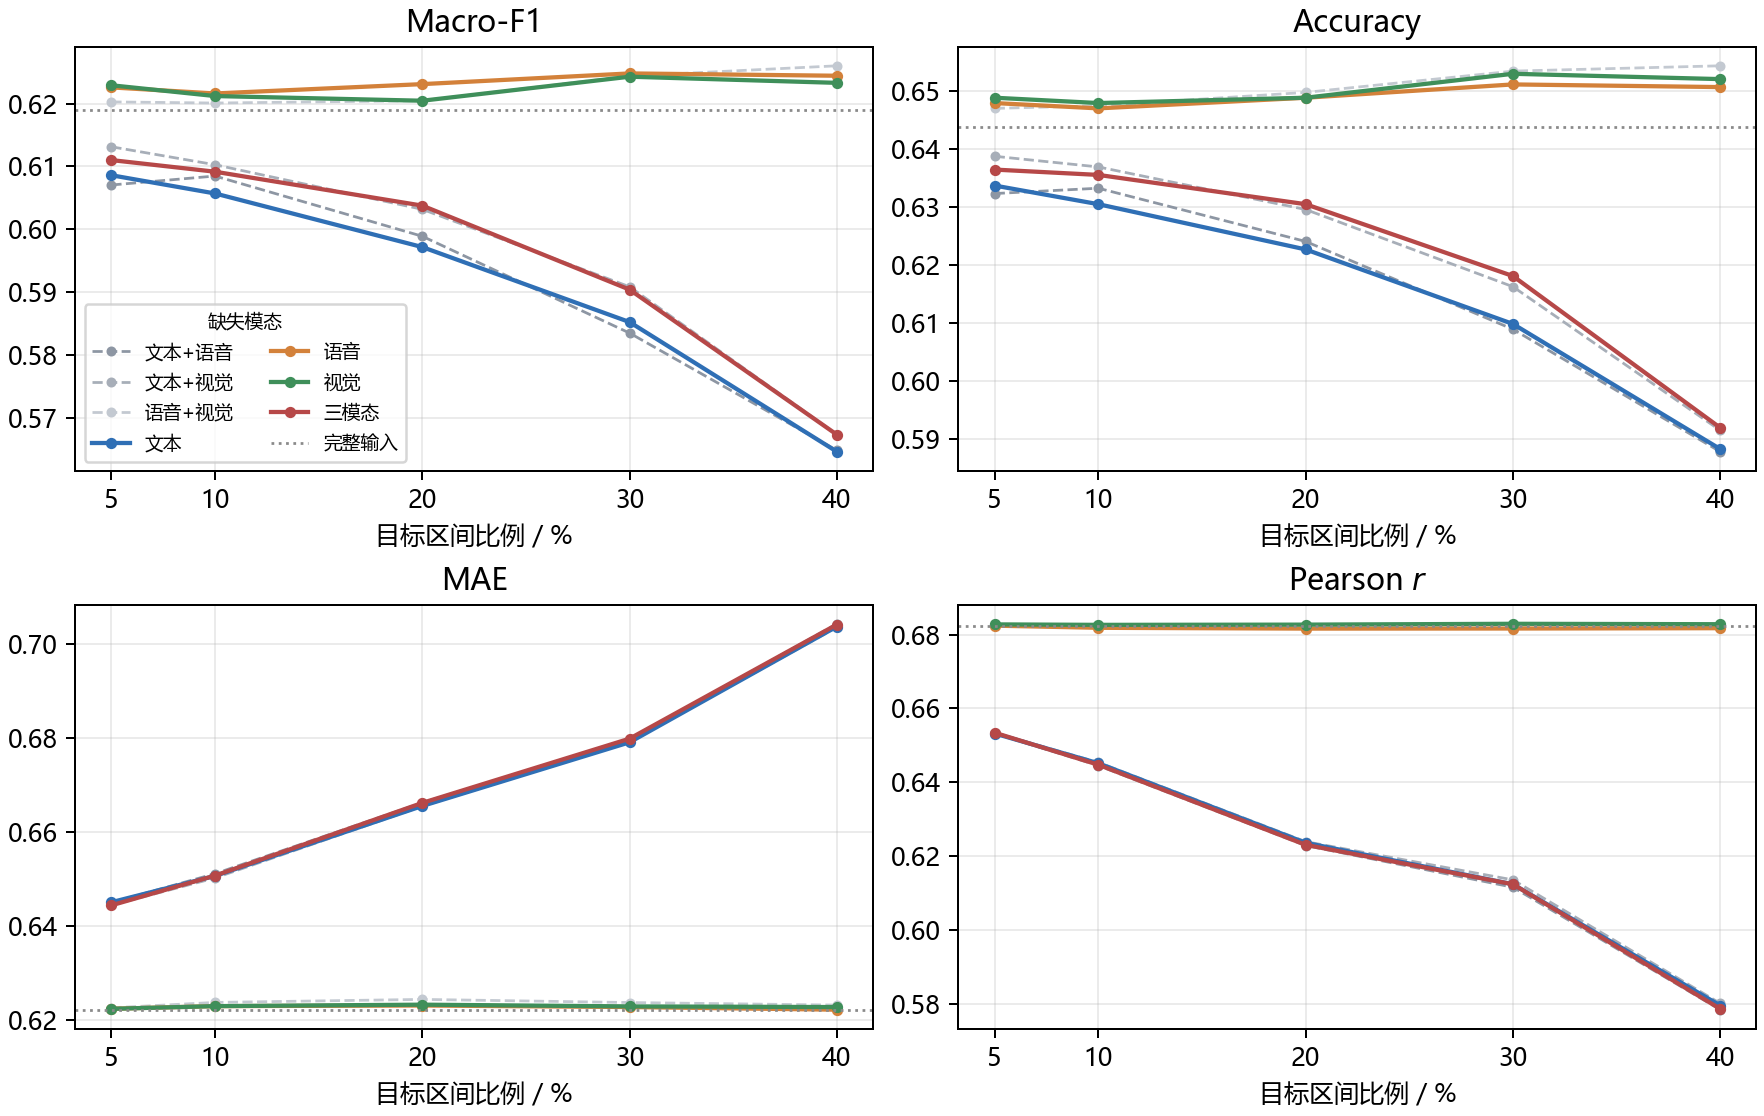
\includegraphics[width=0.9\linewidth]{figures/q2_v4_missing.png}
\caption{不同缺失模态与目标区间比例下四项指标的退化曲线}\label{q2:fig:metriccurve}
\end{figure}

句首缺失的平均F1最高、句中最低，两者相差0.0090；同一位置内部不同模态组合与比例造成的F1跨度远大于位置之间的差异（图\ref{q2:fig:factors}(a)）。逐样本配对比较中，多数样本的判断不因缺口位置改变，变好与变差的比例接近，说明模型主要依据缺口周边仍然存在的证据作判断，而不依赖缺口在序列中的位置。

\begin{figure}[htbp]\centering
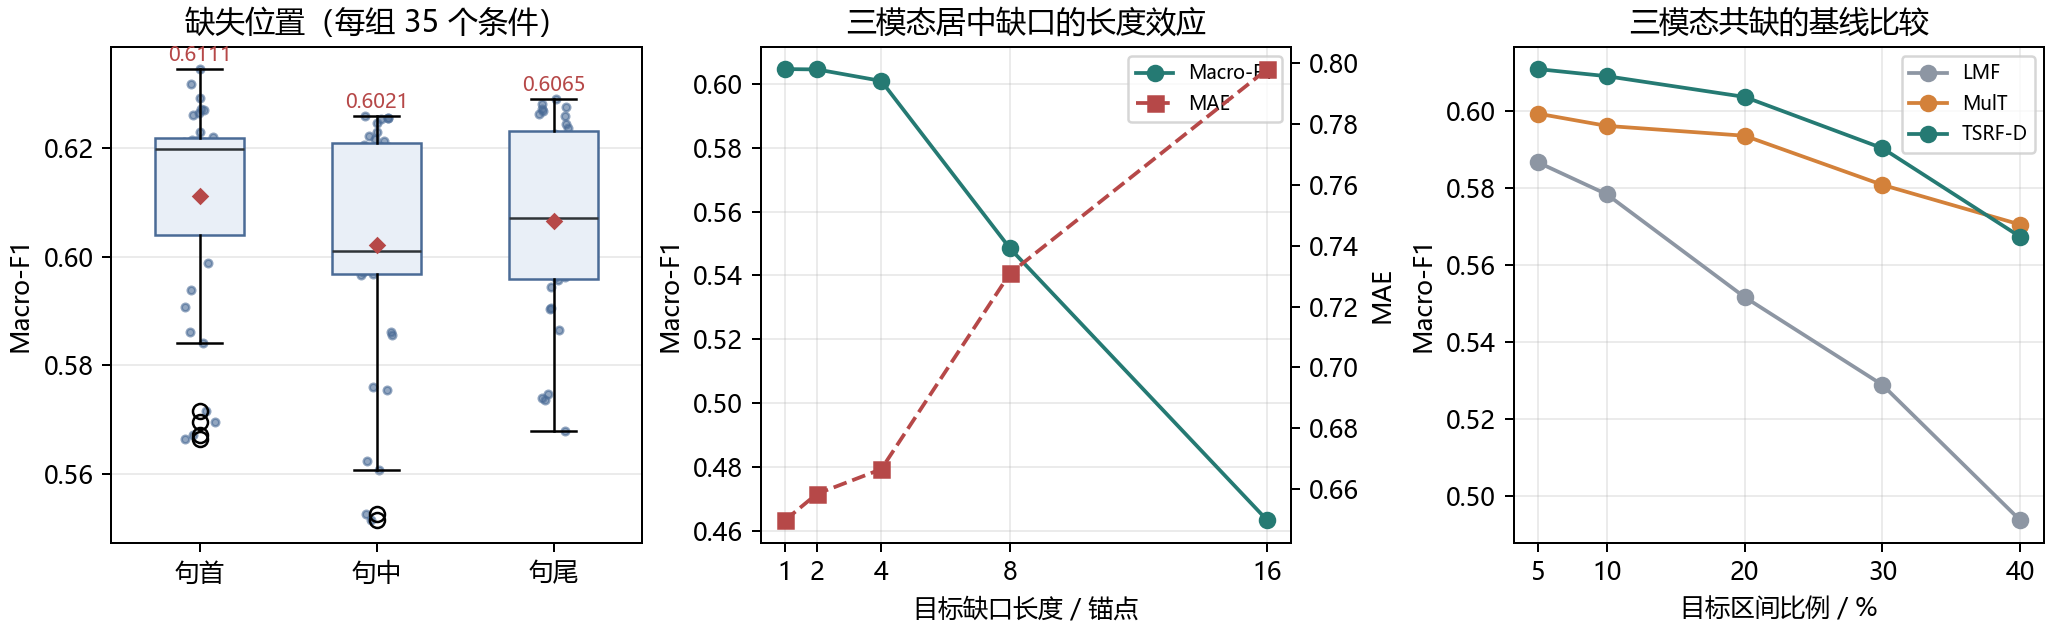
\includegraphics[width=0.9\linewidth]{figures/q2_v4_factors.png}
\caption{缺失位置、缺口长度与基线比较}\label{q2:fig:factors}
\end{figure}


图\ref{q2:fig:factors}(b)给出三模态同段居中缺口的长度效应：F1由长度1锚点的0.6047降至长度16锚点的0.4632，MAE同步上升，缺口由短到长，分类与回归的退化都随之加深，长度4以内的条件仍保持0.60以上的F1。长度以附件提供的对齐锚点度量，短样本的缺口被截为$L_i-1$以保证至少保留一个观测，长度档位越高，受此限制的样本越多。对所选模态实际发生删除且仍保留观测的样本取105种条件的交集，得到648条严格局部样本；在该子集上，LMF、MulT与TSRF-D的平均F1排序与全集口径一致，说明长度效应的结论不依赖样本集合的选择。

图\ref{q2:fig:factors}(c)在三模态同段共缺下给出与两种公开融合基线的对比：缺口越重，方法差距越大。随着目标比例由5\%增至40\%，LMF的Macro-F1持续下降，与TSRF-D的差距扩大到三倍以上；MulT在全比例区间内与TSRF-D接近，两者差值不超过0.013。

\paragraph{受控缺口下的逐样本错误转移}

把完整输入与受控缺口下的判断逐样本对照，测试样本可分为两侧均正确、翻转、修复与两侧均错误四类；翻转样本随缺口比例与缺口长度的增加而单调上升，其中约一半在完整输入下本已判错（图\ref{q2:fig:errors}）。文本单模态缺口与三模态共缺的翻转数量接近，语音与视觉单模态缺口几乎不产生翻转，与模态消融的趋势一致。

\begin{figure}[htbp]\centering
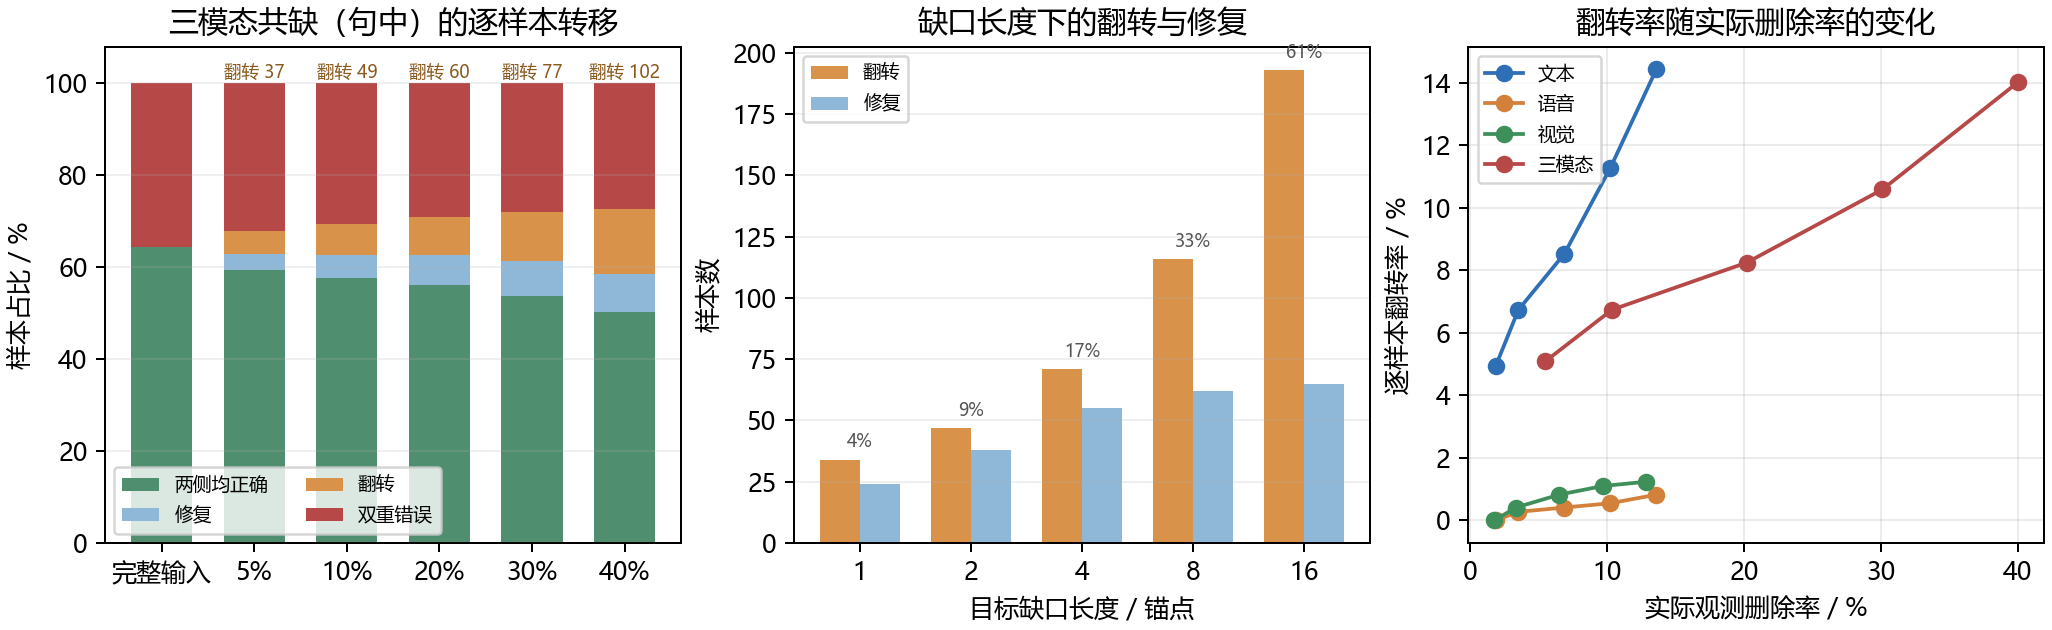
\includegraphics[width=0.9\linewidth]{figures/q2_v4_errors.png}
\caption{受控缺口下的逐样本错误转移}\label{q2:fig:errors}
\end{figure}


\paragraph{验证集可视化与错误归因}

图\ref{q2:fig:valid}给出验证集的类别混淆与强度回归结果。分类误差主要集中在中性边界。负向与正向类的F1明显高于中性类，全部误判中有78.0\%涉及中性，其中多数是真实正向或负向被判为中性；中性样本的强度标签集中在0附近，与相邻极性的表达差别较小，边界样本的极性区分本身较难。强度散点显示连续预测与标签同样在中性附近偏离最大，说明改进空间集中在中间类别而非两端。

\begin{figure}[htbp]\centering
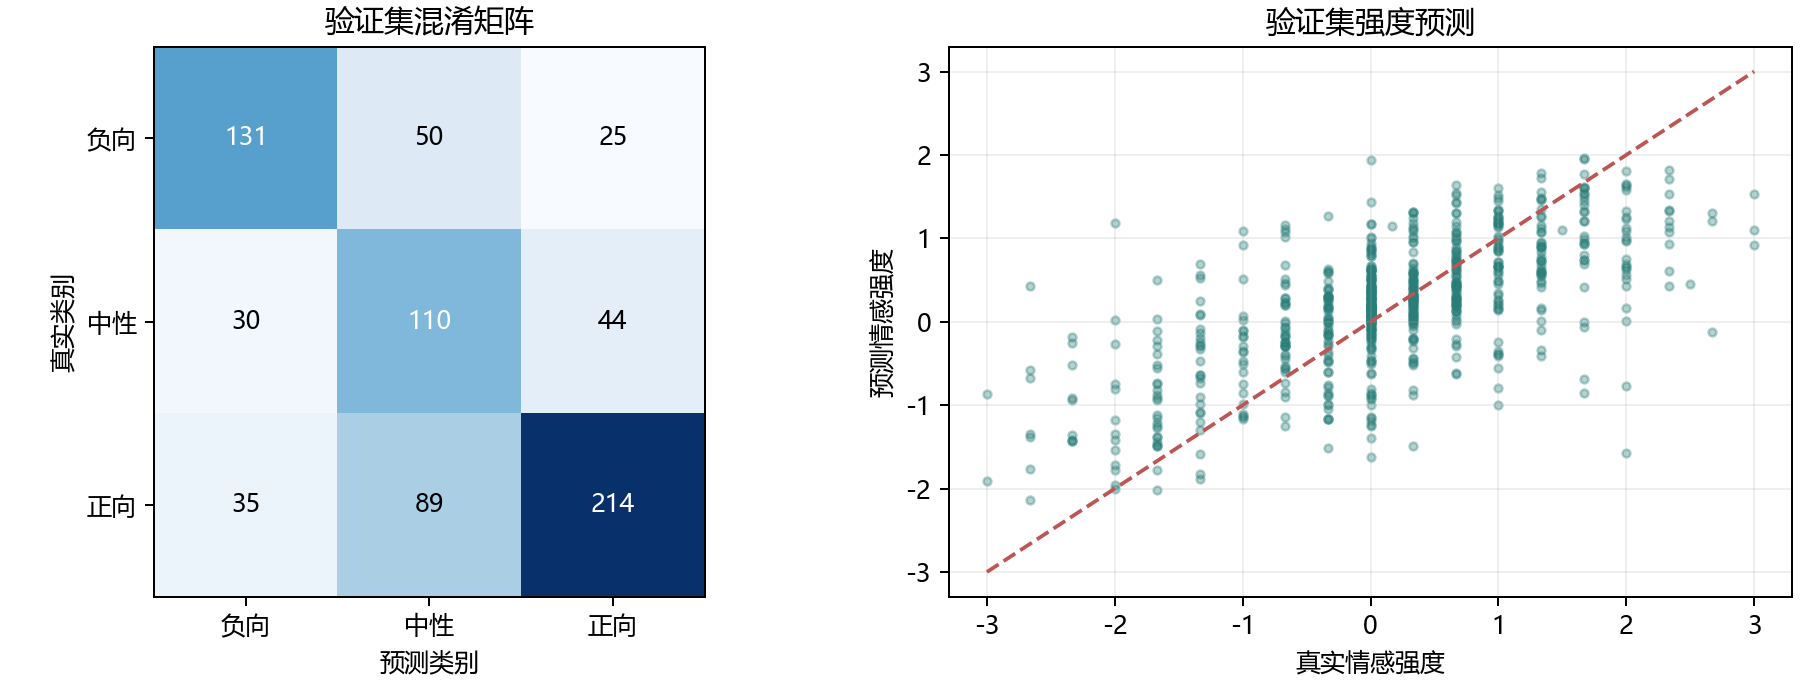
\includegraphics[width=\linewidth]{figures/q2_v4_validation.png}
\caption{验证集类别混淆与强度回归结果}\label{q2:fig:valid}
\end{figure}

\FloatBarrier\subsubsection{与基线的测试集比较}

\paragraph{对照设置}
本节回答两个问题：缺口条件下本文模型相对十类基线是否占优，优势出现在哪一类指标上。比较在同一训练划分、同一遮挡课程、同一冻结文本编码、同一训练集标准化统计量与同样三个种子下重跑，覆盖七类输入处理与结构方案：仅文本、拼接MLP、零填充、均值填充、缺失标记、模态丢弃与三态嵌入；公开融合基线LMF与MulT按本题的三分类与连续回归任务适配，保留各自原有配置。七类输入方案对缺失的处理分为两组：零填充、均值填充、缺失标记与模态丢弃决定缺口处取什么值或留什么标记，仅文本、拼接MLP与三态嵌入决定模态证据以何种形式进入判别模型。自然缺失位置的填充按各模型自身的训练口径执行：零填充使用原始零值，其余模型使用训练集均值。十类模型共用同一批测试样本、同一套人工掩码与三个种子，在基础输入与全部连续局部缺失条件下比较，分类概率与强度输出分别取种子集成，指标差异只来自各模型处理同一缺失结构的方式。

LMF、MulT与内部基线只接受自身监督信号，TSRF-D在此基础上还使用了EMT-DLFR教师的软监督，因此本节比较的是含蒸馏的完整方法与各类基线之间的差距，其训练代价相应包含教师的学习过程。

\begin{table}[htbp]\centering\small
\caption{测试集统一口径的基线比较}\label{q2:tab:baseline}
\begin{tabular}{lrrrrrr}\toprule
模型 & 基础Acc & 基础F1 & 基础MAE & 基础$r$ & 局部F1 & 局部MAE\\\midrule
仅文本 & 0.6410 & 0.6192 & 0.6396 & 0.6613 & 0.6028 & 0.6700\\
拼接MLP & 0.6039 & 0.5805 & 0.6386 & 0.6602 & 0.5852 & 0.6636\\
零填充 & 0.6231 & 0.5894 & 0.6417 & 0.6703 & 0.5851 & 0.6653\\
均值填充 & 0.6410 & 0.6073 & 0.6539 & 0.6659 & 0.5979 & 0.6786\\
缺失标记 & 0.6217 & 0.5945 & 0.6337 & 0.6732 & 0.5900 & 0.6610\\
模态丢弃 & 0.6190 & 0.5855 & 0.6314 & 0.6765 & 0.5782 & 0.6559\\
三态嵌入 & 0.6424 & 0.6078 & 0.6412 & 0.6726 & 0.5976 & 0.6676\\
LMF & 0.6259 & 0.5932 & 0.6729 & 0.6292 & 0.5669 & 0.7028\\
MulT & 0.6437 & 0.6155 & 0.6740 & 0.6509 & 0.5984 & 0.6907\\
TSRF-D & 0.6437 & 0.6189 & 0.6221 & 0.6824 & 0.6066 & 0.6492\\
\bottomrule\end{tabular}\end{table}

\paragraph{基础输入与局部缺失下的表现}
表\ref{q2:tab:baseline}给出十类模型在基础输入与局部缺失条件下的分类与回归指标。基础输入下各模型的分类差距有限，回归差异更清楚。TSRF-D的Accuracy与MulT并列最高，强度MAE与Pearson相关系数两项都优于其余模型，Macro-F1与仅文本几乎相同，配对区间跨零。连续量的预测同时依赖三路通道的完整程度，因此强度指标对输入处理方式的差别更敏感；方法的差别更多体现在人工缺口出现之后。

局部缺失条件下，本文模型在两类指标上均保持领先。全部连续缺失条件的平均F1为0.6066、平均MAE为0.6492，两项在十类模型中均为最优，且相对九类基线的点估计方向一致（表\ref{q2:tab:baseline}）。把基础输入与局部缺失两个水平并置可以看出，起点相近的模型对缺口的耐受并不等价：MulT的基础F1与TSRF-D接近，缺口下差距扩大；均值填充与三态嵌入的局部表现也低于各自的基础水平；LMF在两类输入下都落后，缺口越重差距越大。缺口造成的信息损失能否被补偿，是这一组比较要回答的问题。

经配对检验与Holm校正后，相对模态丢弃的局部F1改善成立，相对均值填充、三态嵌入、LMF与MulT的局部MAE改善同样达到5\%显著性水平（表\ref{q2:tab:paired}）；分类方向的其余比较区间跨零，差异落在评价样本的不确定性范围内。分类上的差异幅度整体小于回归：点估计最大的几项分别对应模态丢弃、零填充与拼接MLP，校正后仅相对模态丢弃的改善达到显著，回归指标的改善覆盖范围更广。强度是连续量，对观测丢失的反应比离散判决更直接，配对差异因此在回归指标上更为明显，结论按各自指标分别给出。

\begin{table}[htbp]\centering\small
\caption{测试集上本文模型相对各基线的局部配对差异及95\%区间}\label{q2:tab:paired}
\begin{tabular}{llrrr}\toprule
基线 & 指标 & 差值 & 95\%区间 & 校正$p$\\\midrule
模态丢弃 & 局部F1 & +0.0284 & [+0.0143, +0.0421] & 0.018\\
模态丢弃 & 局部MAE & -0.0067 & [-0.0194, +0.0061] & 1.000\\
缺失标记 & 局部F1 & +0.0166 & [+0.0019, +0.0325] & 0.684\\
缺失标记 & 局部MAE & -0.0118 & [-0.0222, -0.0017] & 0.480\\
拼接MLP & 局部F1 & +0.0214 & [+0.0029, +0.0406] & 0.513\\
拼接MLP & 局部MAE & -0.0144 & [-0.0291, +0.0001] & 0.856\\
零填充 & 局部F1 & +0.0215 & [+0.0075, +0.0362] & 0.091\\
零填充 & 局部MAE & -0.0161 & [-0.0270, -0.0054] & 0.100\\
三态嵌入 & 局部F1 & +0.0090 & [-0.0031, +0.0209] & 1.000\\
三态嵌入 & 局部MAE & -0.0184 & [-0.0275, -0.0090] & 0.018\\
仅文本 & 局部F1 & +0.0038 & [-0.0166, +0.0232] & 1.000\\
仅文本 & 局部MAE & -0.0208 & [-0.0412, -0.0014] & 0.697\\
均值填充 & 局部F1 & +0.0086 & [-0.0038, +0.0213] & 1.000\\
均值填充 & 局部MAE & -0.0294 & [-0.0413, -0.0177] & 0.018\\
MulT & 局部F1 & +0.0082 & [-0.0080, +0.0254] & 1.000\\
MulT & 局部MAE & -0.0414 & [-0.0598, -0.0235] & 0.018\\
LMF & 局部F1 & +0.0397 & [+0.0152, +0.0633] & 0.056\\
LMF & 局部MAE & -0.0536 & [-0.0783, -0.0276] & 0.018\\
\bottomrule\end{tabular}\end{table}

\begin{samepage}
为量化差异的不确定性，将测试集按来源视频分组进行2000次配对bootstrap；同一视频的不同片段、同一片段的不同缺失条件共用重采样权重，避免相关内容被重复计入。表中差值为本文模型减去基线，F1正值和MAE负值分别表示改善，行序按局部MAE差距由小到大排列，多重比较采用Holm校正。九类基线中，分类方向以仅文本与MulT最接近本文模型，回归方向以模态丢弃最接近，这三处的区间都跨过零线；LMF在两项上的差距都是最大。\par\end{samepage}


\paragraph{输入处理策略的比较}
零填充与均值填充以与位置无关的常量替代观测：前者把缺口推向标准化空间的原点，后者使其回到训练集中心，缺口的位置、长度与周边可用证据都不参与替代值的形成。可学习缺失标记把缺失状态交给模型自行编码，训练期模态丢弃直接移除整路模态，两者给出“此处不可信”的开关，却不回答该处应当依据什么判断。三态嵌入在此基础上区分结构填充、自然缺失与人工缺口，是内部基线中最接近本文模型的配置，但其作用仍停留在状态层面，无法补偿连续缺口丢失的证据。缺口上下文编码与门控补全正对应这一环节：模型由缺口两侧的可用观测生成补全查询，再按可靠度门控在补全结果与上下文回退表示之间取舍。

与公开基线的比较同样支持这一判断：MulT的局部F1与TSRF-D接近而局部MAE差距明显，LMF在两项上都落后。两种融合框架都建立在模态间逐位置对应的联合表示上，缺口使这段对应关系断开，LMF的低秩分解与MulT的跨模态注意力都缺少可用的输入；TSRF-D先在缺口处重建替代证据再作融合，缺口越重，差距越明显。强度回归上的差距比分类更清楚，与连续量对缺失观测的依赖更强有关。


TSRF-D的单种子局部F1标准差为0.0038，与拼接MLP、仅文本同处最低区间；零填充的波动为0.0181，明显高于上述方案，而它恰好也是局部F1最低的方案之一，均值与稳定性同时落后。种子集成降低了初始化差异带来的波动，但不同缺失处理方式之间的稳定性差别仍然保留：缺口处是否有可用的替代表示，同时关系到预测水平与训练的可复现程度。

\paragraph{缺失条件下的鲁棒性概括}

把四组实验合起来看，模型在局部缺失下保持稳定输出。全部连续缺失条件的等权平均结果在十类模型中均为最优，相对主要基线的改善经来源视频分组配对检验与多重比较校正后成立；退化随缺失程度单调但幅度有限，目标比例上升造成的累计下降不足百分之三，缺口位置的影响更小，逐样本比较中多数判断不变且变好与变差的比例接近，没有方向性偏置。缺口越重，相对通用融合框架的优势越大；退化几乎全部来自覆盖样本主体的文本长缺口，语音与视觉单模态缺口在各比例上几乎不改变输出。在题目定义的局部缺失范围内，模型对缺失类型、位置与比例的变化保持稳定输出。

\FloatBarrier\subsubsection{附件3全量预测与结果展示}

冻结模型后对附件3全部30条样本完成推理，预测分布为负向7条、中性9条、正向14条；缺失在同一时段跨模态重合，三路缺失计数在29条样本上完全一致，与训练中多模态同段缺失的形态相符。附件3没有真实标签，分类概率只反映模型输出分布，不用于计算准确率。

图\ref{q2:fig:a3}左栏为30条样本的三类概率热图，行按样本编号排列、颜色越深表示该类别的概率越高；右栏给出强度预测与种子间标准差。缺失位置少的样本，最大类别概率与强度绝对值都更高；缺失超过8个位置的样本两项明显下降，低置信样本全部落在缺失较多的范围内。可用观测减少时，类别分布更平坦，强度取值也更靠近零。

30条样本中仅3-22一条的类别方向与强度符号不一致：该样本判为负向而强度为$+0.0834$，数值离零很近，处于中性边界附近，软一致性约束下两个头在边界样本上仍保留各自的判断。其余样本的极性方向与强度符号一致，强度绝对值较大的样本最大类别概率同样较高。

\begin{figure}[htbp]\centering
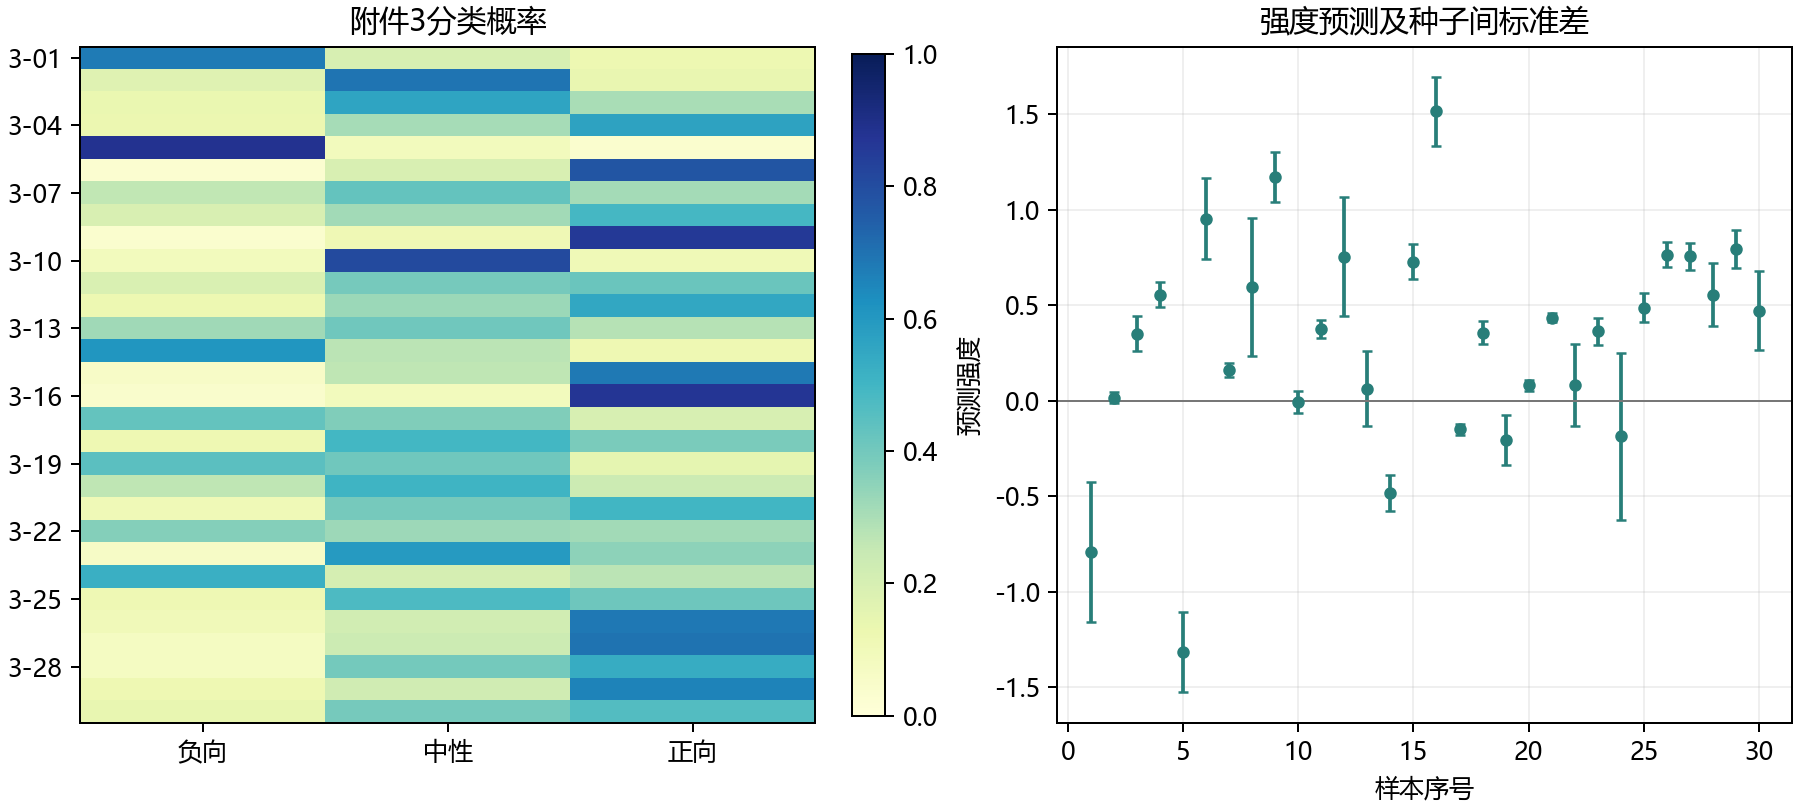
\includegraphics[width=\linewidth]{figures/q2_v4_a3.png}
\caption{附件3全量样本的分类概率与强度预测}\label{q2:fig:a3}
\end{figure}


表\ref{q2:tab:a3}逐条列出全部30条样本的可用锚点数、三路缺失位置计数、预测极性、连续强度与最大类别概率；锚点数与缺失计数共同刻画每条样本的可用证据规模，最大概率给出类别判断的集中程度。

\begingroup
\small
\setlength{\tabcolsep}{6pt}
\begin{longtable}{lrllrr}
\caption{附件3全部30条样本的预测}\label{q2:tab:a3}\\
\toprule
样本 & 锚点数 & 缺失$t/a/v$ & 极性 & 强度 & 最大概率\\
\midrule
\endfirsthead
\caption*{续表\ \thetable}\\
\toprule
样本 & 锚点数 & 缺失$t/a/v$ & 极性 & 强度 & 最大概率\\
\midrule
\endhead
3-01 & 6 & 0/0/0 & 负向 & -0.7926 & 0.6790\\
3-02 & 28 & 5/5/5 & 中性 & +0.0170 & 0.6927\\
3-03 & 32 & 5/5/9 & 中性 & +0.3507 & 0.5615\\
3-04 & 31 & 2/2/2 & 正向 & +0.5548 & 0.5655\\
3-05 & 12 & 0/0/0 & 负向 & -1.3149 & 0.8804\\
3-06 & 25 & 3/3/3 & 正向 & +0.9528 & 0.7760\\
3-07 & 21 & 3/3/3 & 中性 & +0.1607 & 0.4278\\
3-08 & 15 & 2/2/2 & 正向 & +0.5953 & 0.4915\\
3-09 & 14 & 2/2/2 & 正向 & +1.1710 & 0.8556\\
3-10 & 6 & 0/0/0 & 中性 & -0.0066 & 0.8054\\
3-11 & 14 & 4/4/4 & 正向 & +0.3761 & 0.4166\\
3-12 & 13 & 2/2/2 & 正向 & +0.7533 & 0.5491\\
3-13 & 19 & 2/2/2 & 中性 & +0.0642 & 0.4059\\
3-14 & 23 & 2/2/2 & 负向 & -0.4828 & 0.6079\\
3-15 & 27 & 3/3/3 & 正向 & +0.7277 & 0.6803\\
3-16 & 34 & 4/4/4 & 正向 & +1.5138 & 0.8705\\
3-17 & 22 & 8/8/8 & 负向 & -0.1494 & 0.4290\\
3-18 & 17 & 3/3/3 & 中性 & +0.3571 & 0.4949\\
3-19 & 24 & 7/7/7 & 负向 & -0.2043 & 0.4454\\
3-20 & 48 & 14/14/14 & 中性 & +0.0810 & 0.5071\\
3-21 & 9 & 3/3/3 & 正向 & +0.4352 & 0.4968\\
3-22 & 17 & 4/4/4 & 负向 & +0.0834 & 0.3645\\
3-23 & 13 & 4/4/4 & 中性 & +0.3641 & 0.5916\\
3-24 & 8 & 2/2/2 & 负向 & -0.1855 & 0.5218\\
3-25 & 9 & 2/2/2 & 中性 & +0.4876 & 0.4757\\
3-26 & 22 & 6/6/6 & 正向 & +0.7644 & 0.6848\\
3-27 & 21 & 8/8/8 & 正向 & +0.7554 & 0.6965\\
3-28 & 33 & 11/11/11 & 正向 & +0.5554 & 0.5326\\
3-29 & 18 & 8/8/8 & 正向 & +0.7940 & 0.6596\\
3-30 & 24 & 12/12/12 & 正向 & +0.4701 & 0.4629\\
\bottomrule
\end{longtable}
\endgroup


\FloatBarrier

\subsection{问题三的模型建立与求解}
\label{sec:q3}
\FloatBarrier
\subsubsection{问题分析与建模思路}
问题三针对三模态信息完整而决策依据难以追溯的场景，要求在输出情感极性与连续强度的同时，以可量化、可复核的方式给出判断依据：量化各模态在当前样本中的作用差异，明确主要参考模态，定位各模态中与判断密切相关的局部片段，并使关键证据能够对应至原始文本片段、语音时段或视觉关键帧。本问使用附件2提供的对齐版特征训练预测器，训练、验证与测试样本分别为3395、728与727条，并对附件4的全部20条无标签样本完成预测与解释。

与问题二处理证据不完整不同，本问的难点在于把“判断依据”转化为可计算的量。模态作用差异是整体量，局部证据是片段量，两者粒度不同，需要在不同层级分别定义；删除输入会改变模型看到的样本，若预测器只在完整输入上训练，删除后的输出变化将同时包含证据缺失与输入分布变化两种效应，难以单独归因。此外，显眼的片段与真正改变输出的片段并不一致，解释结果需要经过删除型检验才能确认其与模型决策的对应关系。证据还必须能够回到原始素材，这要求解释结果沿词级时间区间与视频时间戳逐级映射，而不是停留在特征下标。

据此，本文采用以同一预测器支撑预测与解释、以两级输入干预定义判断依据的建模方案，建立输入干预联盟Shapley解释模型（ICF-Shapley），按“情感预测、模态贡献分解、局部证据定位、原素材回映”四个步骤求解。预测器采用子集感知结构（SAP），以三态输入与逐模态双向时序编码输出极性与强度，训练时按模态联盟采样：以0.70的概率保留全部模态，其余概率均匀分配给7个非完整联盟，使模型在任意可用子集下都保持有效输出。模型关闭补全分支，被删除位置不再获得替代表示，干预后的输入状态完全由观测掩码决定，删除响应因此对应“证据不可用”本身。模态层对文本、语音和视觉的8个联盟精确枚举，以Shapley值分配预测变化并核验效率性，由贡献确定作用份额与主要参考模态；片段层将内容区划分为互不重叠的2锚点块，逐块删除并以固定参考类别的输出变化作为局部响应，符号区分支持与抑制。沿用前两问的内容掩码、观测掩码与词级时间区间记号，两级解释在同一冻结预测器上完成。总体结构如图\ref{q3:fig:arch}所示。

模型在50个对齐锚点上统一输出；解释评价从分解性质、忠实性与稳定性三个方面展开：Shapley分解检验效率性，局部证据以高分块与随机块、低分块的累计删除曲线差（AOPC）与条件充分性度量，稳定性由多种子主模态一致率与替代基线对照检验。最后按块内原词的CTC时间区间回映证据时段，提取对应音轨与最近PTS关键帧，完成附件4全量样本的预测、解释与回映核验。

\subsubsection{数据准备}
\FloatBarrier
\paragraph{输入组织与可用模态}
采用附件2的对齐版特征，共4850条样本，按官方划分使用3395条训练样本、728条验证样本与727条测试样本。三模态输入张量分别为$X^t\in\R^{50\times768}$、$X^a\in\R^{50\times74}$、$X^v\in\R^{50\times35}$，标签包含三分类极性与连续情感强度，分类与回归在同一输入上联合求解。文本输入由附件2的词元编号经冻结的\file{bert-base-uncased}重算得到，训练与解释干预共用同一编码接口；语音与视觉特征按锚点整体给出，模型不再细分锚点内部的帧。

以$P_{ik}$表示内容掩码，$O^m_{ik}$表示模态$m$的观测掩码；标准化统计量仅由训练集观测位置估计，附件4沿用同一组统计量。附件4包含20条无标签样本，共564个内容锚点，单条长度介于11与48之间，只参与前向预测与解释，不用于训练、选模与阈值确定。按赛题定义，附件4为三模态信息完整的真实场景数据；直接读取官方特征文件时，第13条的视觉特征在全部30个内容位置均为零，本文未对该样本做遮挡或替换，而是按文件实际取值记录该异常，并在后续计算中将该样本的视觉分支标记为不可用。定义
\begin{equation}
L_i=\sum_kP_{ik},\quad \mathcal A_i=\{m\in\mathcal M:\sum_kO^m_{ik}>0\},\quad
\rho_i^m=\frac{\sum_kO^m_{ik}}{L_i},\qquad\mathcal M=\{t,a,v\}.
\end{equation}
其中$L_i$为内容长度，$\mathcal A_i$为可用模态集合，$\rho_i^m$描述观测比例。不可用模态在所有联盟中保持缺失，输出贡献记为NA；该标记描述特征文件的可用性，不能解释为贡献为零。

\FloatBarrier
\paragraph{片段划分与时间回映}
局部解释以内容区内的连续锚点块为单位：将内容区划分为不重叠的2锚点块$E$，末块允许不足2个锚点。块长度取2个锚点，在保持证据定位粒度的同时避免单个位置带来的响应波动。解释时保持序列长度与位置不变，仅改变相应位置的输入与观测状态，删除不引起时间轴错位。文本块先替换为\file{[UNK]}，再对整句重新编码，使被删词的信息不再通过上下文表示残留；语音和视觉块通过观测掩码删除，被删位置的状态转为缺失，其表示由缺失嵌入替代，原始观测值不再进入后续计算。

附件4原始转写与音轨经词级CTC强制对齐，得到原词区间$A_{iu}=[a_{iu},b_{iu})$；词表构建与对齐直接调用问题一的模块，使解释证据与前问的时序基准一致。若块$E$对应原词集合$\mathcal U_i(E)=\{g_i(k):k\in E\}$，则证据时间范围为
\begin{equation}
I_i(E)=\left[\min_{u\in\mathcal U_i(E)}a_{iu},\ \max_{u\in\mathcal U_i(E)}b_{iu}\right).
\end{equation}
包含部分子词时按所属原词完整区间回映；逐位核验分词序列后，以块内已对齐实词区间的包络定位证据。标点保留在文本与锚点索引中，不单独赋予发音时间；若块内含有未对齐实词，则保留锚点并标记未映射。按真实视频PTS提取距区间中点最近的关键帧，同时导出对应音轨，使每条证据都能回看至原始素材。CTC区间为自动估计，回映覆盖率度量证据的可追溯性。

\FloatBarrier
\subsubsection{模型构建}
\FloatBarrier
\paragraph{总体结构与解释接口}
图\ref{q3:fig:arch}给出问题三的预测器与解释层结构。模型先以三态观测输入完成情感预测，再在同一冻结预测器上分别进行模态联盟干预和局部片段干预；前者输出模态贡献与主要参考模态，后者输出关键证据位置，最后通过词级时间区间和视频PTS回映至原始素材。解释层不另行训练预测器，因而解释结果与预测结果来自同一模型输出。

预测器只保留三态投影、时序编码、模态池化与双任务头，不含补全、门控与蒸馏分支，被删除的信息在后续计算中保持缺失，不会被重建路径补回，删除响应因此对应输入证据本身的变化。两级干预面向两种解释粒度：模态层回答当前判断主要依赖哪一路信息，片段层回答该路信息中的哪些词或时段起了作用；二者的干预对象与价值函数分别定义，整体贡献与局部证据不相互混入。

\begin{figure}[H]\centering
\begin{tikzpicture}[font=\small,
 box/.style={draw=black!65,fill=black!3,text width=8.8cm,align=center,minimum height=8mm,inner sep=4pt},
 branch/.style={draw=black!65,fill=black!3,text width=4.0cm,align=center,minimum height=12mm,inner sep=4pt},
 arr/.style={-{Latex[length=2mm]},thick}]
\node[box] (x) {三模态对齐特征：内容掩码、观测掩码、三态输入};
\node[box,below=4mm of x] (e) {模态投影 + 位置、模态和状态嵌入};
\node[box,below=4mm of e] (g) {逐模态BiGRU + 内容位池化 + 可用比例};
\node[box,below=4mm of g] (h) {共享融合表示：分类概率 $p$ 与强度 $\hat r$};
\node[branch,below=9mm of h.south,xshift=-24mm] (m) {模态联盟干预\\8个联盟精确枚举};
\node[branch,below=9mm of h.south,xshift=24mm] (b) {局部片段干预\\2锚点块逐块删除};
\node[branch,below=6mm of m] (o1) {Shapley贡献、作用份额\\主要参考模态};
\node[branch,below=6mm of b] (o2) {局部响应与关键片段\\时间区间与关键帧回映};
\draw[arr] (x)--(e);\draw[arr] (e)--(g);\draw[arr] (g)--(h);
\draw[arr] (h)--(m);\draw[arr] (h)--(b);\draw[arr] (m)--(o1);\draw[arr] (b)--(o2);
\end{tikzpicture}
\caption{问题三ICF-Shapley预测器与解释层结构}\label{q3:fig:arch}
\end{figure}

\FloatBarrier
\paragraph{三态投影与时序编码}
令$s^m_{ik}\in\{0,1,2\}$分别表示结构填充、已观测和内容缺失。三种状态各有一套嵌入，使模型能够区分“该位置不存在”与“该位置存在但观测不可用”。最终采用单层预测器，其输入表示为
\begin{equation}
z^m_{ik}=\operatorname{Lin}_m(X^m_{ik})+e_m^{\mathrm{mod}}+e_k^{\mathrm{pos}}+e^{\mathrm{state}}_{s^m_{ik}},\qquad
\widetilde z^m_{ik}=O^m_{ik}z^m_{ik}+P_{ik}(1-O^m_{ik})e_m^{\mathrm{miss}}.
\end{equation}

缺失位置由模态相关的缺失嵌入$e_m^{\mathrm{miss}}$替代：序列长度与位置索引保持不变，删除只在输入取值层面生效，不改变时间轴。按内容长度打包序列，分别输入逐模态双向GRU，避免结构填充参与递归。设隐藏维度为$d$，对各模态内容位的编码结果$h^m_{ik}$分别取均值与最大值，再拼接观测比例：
\begin{equation}
u_i=\operatorname{Concat}_{m\in\mathcal M}\left(\frac1{L_i}\sum_kh^m_{ik},\max_kh^m_{ik}\right)
\mathbin\Vert[\rho_i^t,\rho_i^a,\rho_i^v],\qquad h_i=\operatorname{MLP}(u_i).
\end{equation}

均值概括模态内部的总体倾向，最大值捕捉局部显著响应，观测比例$\rho_i^m$给出该模态证据的可用程度，三者共同形成样本级表示。融合向量维度为$6d+3$，分类与回归头分别输出
\begin{equation}
p_i=\operatorname{softmax}(W_ch_i+b_c),\qquad \widehat r_i=3\tanh(W_rh_i+b_r).
\end{equation}

强度输出经$3\tanh$限幅至$[-3,3]$，与标签取值范围一致。

\FloatBarrier
\paragraph{子集训练与目标函数}
解释层需要对任意模态联盟求值：Shapley贡献要在全部8个子集上计算输出，片段删除也要求模型在部分观测缺失时仍然有效。若只在完整输入上训练，联盟输入会成为分布外样本，输出变化将混入分布外效应。为此按原训练分布设置对照配置C0：以0.70的概率保留全部模态，其余0.30均匀分配给7个非完整联盟，包含空集；完整输入保持为主要训练分布，非完整组合同时进入训练。对采样联盟$S_i$，令$\widetilde O^m_{ik}=O^m_{ik}\mathbf1\{m\in S_i\}$。训练目标为
\begin{equation}
\mathcal L_3=\operatorname{CE}_w(y_i,p_i)+\operatorname{Huber}_1(r_i,\widehat r_i)
+0.2\left[(p_{i,+}-p_{i,-})-\tanh(\widehat r_i/3)\right]^2.
\end{equation}

类别权重由训练集频数确定，缓解三类样本不均衡；Huber损失拟合连续强度，对大偏差样本保持稳健；最后一项约束正向与负向概率之差同强度符号的方向一致性，使两个输出头在同一表示上协同。该方案覆盖模态联盟输入；连续片段遮挡增广及更深网络作为候选变体单独比较。

\FloatBarrier
\paragraph{模态贡献与主要参考模态}
以三种子平均概率$\bar p_i$确定原始可用输入的参考类别$c_i^*=\arg\max_c\bar p_{ic}(\mathcal A_i)$，解释全过程固定该类别，使所有干预以同一决策为比较对象，避免类别切换混入贡献。对联盟$S\subseteq\mathcal M$，定义
\begin{equation}
F_i^{\mathrm{cls}}(S)=\log\frac{\bar p_{i,c_i^*}(S)}{1-\bar p_{i,c_i^*}(S)},\qquad
F_i^{\mathrm{reg}}(S)=\overline{\widehat r}_i(S).
\end{equation}

概率经log-odds变换到无界尺度，价值差可以直接相减；数值计算时将概率截断至$[10^{-6},1-10^{-6}]$以保证稳定。对分类与强度分别计算Shapley贡献：
\begin{equation}
\phi_i^m=\sum_{S\subseteq\mathcal M\setminus\{m\}}\frac{|S|!(2-|S|)!}{3!}
\left[F_i(S\cup\{m\})-F_i(S)\right],\qquad
\sum_{m\in\mathcal A_i}\phi_i^m=F_i(\mathcal A_i)-F_i(\varnothing).
\end{equation}

三个模态只构成8个联盟，可以精确枚举，不需要蒙特卡洛近似；效率性等式同时作为实现的数值核验。贡献为正表示相对基线抬高价值，为负表示压低价值。以分类贡献绝对值最大的可用模态为主要参考模态，作用份额定义为
\begin{equation}
m_i^*=\arg\max_{m\in\mathcal A_i}|\phi_i^{m,\mathrm{cls}}|,\qquad
\omega_i^m=\frac{|\phi_i^{m,\mathrm{cls}}|}{\sum_{j\in\mathcal A_i}|\phi_i^{j,\mathrm{cls}}|}.
\end{equation}

有符号贡献描述作用方向，作用份额描述作用大小，两者分别报告。当总贡献幅度小于$10^{-8}$时标记为无法区分。

\FloatBarrier
\paragraph{局部证据与解释评价}
记$F_i^{\mathrm{cls,del}(m,E)}$为仅删除模态$m$中块$E$后的固定类别价值，定义
\begin{equation}
\Delta_i^m(E)=F_i^{\mathrm{cls}}(\mathcal A_i)-F_i^{\mathrm{cls,del}(m,E)}.
\end{equation}

$\Delta_i^m(E)>0$表示该片段支持参考类别，小于零表示抑制参考类别。另定义强度响应$\Delta_i^{m,\mathrm{reg}}(E)=\hat r_i-\hat r_i^{\mathrm{del}(m,E)}$，正、负值分别表示该片段抬高、降低预测强度。两个任务分别以贡献绝对值确定主要模态，并在各可用模态中选择绝对局部响应最大的片段作为关键证据，保留符号方向。分类删除检验仍按有符号响应降序，强度删除检验按绝对强度响应排序。

解释评价检验的是证据排序与模型响应是否一致。在主要参考模态中，按块数的10\%、20\%、30\%向上取整，分别累计删除高分块、低分块和随机块；随机顺序重复3次，并报告实际锚点覆盖率。以三个删除档位的平均概率下降定义AOPC，按样本配对比较高分与随机删除，采用2000次bootstrap估计区间：若高分块确实承载判断依据，删除它们造成的参考类别概率下降应大于随机删除。条件充分性保留其他模态及主要模态的高分块，计算相对原预测的绝对概率偏差，考察高分块在多大程度上替代完整输入。另以训练集同位置均值（B2）和模态内顺序打乱（B3）替代缺失状态基线（B1），比较主模态一致率及贡献排序，检验解释结论对基线取法的敏感性。

\FloatBarrier
\subsubsection{模型求解与参数设置}
\FloatBarrier
\paragraph{求解流程}
求解分为训练、选模与解释三个阶段。训练阶段在附件2训练集上按联盟采样学习三种子预测器，标准化统计量由训练集观测位置估计，训练轮次由验证集联合指标早停确定；选模阶段在验证子集上按联合指标与三项门槛比较候选配置，确定最终结构并冻结参数；解释阶段在同一冻结模型上依次完成模态联盟枚举、逐块删除与证据回映：联盟枚举对每个样本的可用模态精确求解Shapley值，并逐样本核验效率性公理，贡献之和与联盟价值之差不超过$8.9\times10^{-16}$；逐块删除在2锚点块粒度上给出有符号响应；证据回映把响应区间映射回原素材，最后对附件4的20条样本输出预测与解释。解释阶段不更新任何参数，不同干预之间的输出差异只来自输入本身的变化。

\paragraph{候选比较与模型选择}
以对照配置C0为基准，设置三个递进变体：V1调整联盟采样并加入连续块遮挡；V2进一步采用两层BiGRU、逐模态LayerNorm和回归支路；V3增加联盟单调一致性正则。V1与V2各包含多项联合改动，因此比较反映方案组合的影响；V3约束增补模态后的参考类别响应，其单调性不等价于贡献可加性。

选模指标为$J=\mathrm{Macro\mbox{-}F1}-0.1\mathrm{MAE}$，同时考察分类与回归：Macro-F1按逐类等权计算，强度误差以0.1的系数扣除，避免选模偏向单一任务。候选须同时满足三项门槛：$J$不低于C0减0.002；去文本、去语音、去视觉及全缺失四种状态的平均Macro-F1不低于C0减0.002；解释AOPC差不低于C0减0.005。前两项约束联盟输入下的预测能力，联盟枚举与片段删除都要求模型在子集输入上保持有效；第三项约束解释忠实性，避免预测指标改善而证据排序退化。通过者按缺失状态平均Macro-F1排序，并列时比较$J$。训练早停与变体选择使用验证集，最终在附件2测试集评价预测性能，对附件4输出预测与解释。

\paragraph{训练与解释参数}
最终预测器的网络规模、训练配置及解释采样参数汇总于表\ref{q3:tab:params}。全集与非完整联盟联合采样，使同一预测器同时学习常规预测和模态删除后的输入状态；训练中三个种子相互独立，各自按验证集$J$保存最优轮次，预测概率与强度输出取均值形成集成。解释阶段冻结全部参数，随机删除顺序与bootstrap重采样均固定种子，使不同干预之间保持可比。解释采样与统计口径在验证子集上确定，测试集与附件4只参与冻结后的前向计算。

\begin{table}[H]\centering\small
\caption{最终SAP预测器与解释参数}\label{q3:tab:params}
\begin{tabularx}{\linewidth}{p{1.5cm}p{3.2cm}Y}\toprule
类别 & 项目 & 设置\\\midrule
模型结构 & 投影与融合 & 公共维度$d=64$；融合MLP；Dropout 0.2\\
 & 时序编码 & 逐模态单层BiGRU，单方向隐维32\\
 & 输出 & 分类softmax；强度$3\tanh$，两任务共享融合表示\\\midrule
训练设置 & 目标函数 & 逆频率类别权重；Huber阈值1；方向一致性系数0.2\\
 & 优化器与调度 & AdamW；学习率0.0015；权重衰减$10^{-4}$；余弦调度\\
 & 批量与轮次 & 批量256；至多32轮；早停耐心8；梯度范数上限5\\
 & 随机种子 & 独立训练0、1、2，三种子输出取均值集成\\\midrule
联盟采样 & 训练分布 & 全集0.70；其余7个联盟各$0.30/7$；无块遮挡增广\\\midrule
解释设置 & 模态层 & 8个联盟精确枚举，逐样本核验效率性\\
 & 片段层 & 2锚点块逐块删除；随机顺序重复3次\\
 & 统计口径 & 删除档位10\%、20\%、30\%；bootstrap 2000次\\
 & 对照基线 & B1缺失状态；B2训练集同位置均值；B3模态内打乱\\\midrule
评价数据 & 验证子集 & 固定种子20260925抽取96条，用于解释诊断与选模\\
 & 确认子集 & 固定种子20261001抽取96条测试样本；区间按原视频聚类\\
 & 计算环境 & Python 3.12；PyTorch 2.8.0+cu128；RTX 5060 Ti\\\bottomrule
\end{tabularx}\end{table}

算法\ref{q3:alg}给出从训练到证据回映的完整流程：先在训练集上完成子集感知预测器的学习与选模，再固定参考类别完成模态层分解，随后逐块删除得到局部响应，最后把证据映射回原始素材。

\begin{algorithm}[H]
\caption{ICF-Shapley预测与证据定位}\label{q3:alg}\small
\textbf{输入：}附件2训练、验证与测试集，附件4样本，三模态特征与掩码，标准化参数，种子集合$\{0,1,2\}$。\par
\textbf{输出：}情感极性与强度、模态贡献$\phi_i^m$、作用份额$\omega_i^m$、主要参考模态$m_i^*$及局部证据。\par
\medskip\noindent
\begin{tabularx}{\linewidth}{@{}r@{\quad}Y@{}}
1 & 仅用训练集观测位置拟合标准化统计量，构建内容掩码$P$与观测掩码$O$。\\
2 & \textbf{对每个}种子$s\in\{0,1,2\}$，\textbf{执行}：按C0联盟采样训练预测器（全集0.70，其余7个联盟各$0.30/7$），按验证集$J$保存最优轮次。\\
3 & 在验证子集上按$J$与三项门槛比较候选配置，确定最终结构并冻结参数。\\
4 & \textbf{对每个}样本$i$，计算可用集合$\mathcal A_i$与三种子集成预测，固定参考类别$c_i^*$。\\
5 & 枚举8个模态联盟（不可用模态保持缺失），计算分类log-odds$F_i^{\mathrm{cls}}(S)$与预测强度$F_i^{\mathrm{reg}}(S)$。\\
6 & 求解两类Shapley值，核验效率性残差，输出$\phi_i^m$、$\omega_i^m$与主要参考模态$m_i^*$。\\
7 & 遍历各可用模态的2锚点块，逐块删除并计算分类响应$\Delta_i^m(E)$与强度响应$\Delta_i^{m,\mathrm{reg}}(E)$。\\
8 & 依绝对响应选择各模态分类与强度的关键证据，保留作用方向。\\
9 & 在主要参考模态按10\%、20\%、30\%累计删除高分块、低分块与随机块，按样本配对计算AOPC与条件充分性。\\
10 & 由原词CTC区间与视频PTS定位证据时段与关键帧，导出对应音轨与解释卡。\\
11 & 保存预测、贡献与逐块响应；在验证子集比较B1/B2/B3基线，冻结后在确认子集核验双任务删除响应与稳定性。\\
\end{tabularx}\par
\end{algorithm}

\FloatBarrier
\subsubsection{实验结果与分析}
\FloatBarrier
\paragraph{预测性能与候选比较}
按三项门槛选择的预测器为C0对照（原训练分布），三个种子各自在验证集上取得最优轮次，训练轮次完全由验证集$J$决定，测试集与附件4只参与前向计算。三种子集成在验证集与测试集上给出接近的分类与回归表现。测试集Macro-F1为0.6054，强度MAE在测试集上略高于验证集，反映强度预测的误差随样本变化有所增加；RMSE与CCC在两个划分上的差异同样有限（表\ref{q3:tab:perf}）。
\begin{table}[H]\centering\small
\caption{SAP三种子集成的预测性能}\label{q3:tab:perf}
\begin{tabular}{lrrrrrrr}\toprule
数据集 & 样本数 & Accuracy & Macro-F1 & MAE & RMSE & Pearson & CCC\\\midrule
验证集 & 728 & 0.6264 & 0.6170 & 0.5954 & 0.8053 & 0.6420 & 0.6067 \\
测试集 & 727 & 0.6286 & 0.6054 & 0.6303 & 0.8627 & 0.6730 & 0.6432 \\
\bottomrule\end{tabular}\end{table}
验证集负向与正向的F1明显高于中性，中性边界的刻画是提升分类表现的关键环节。图\ref{q3:fig:perf}给出类别间的混淆结构与各类别指标。
\begin{figure}[H]\centering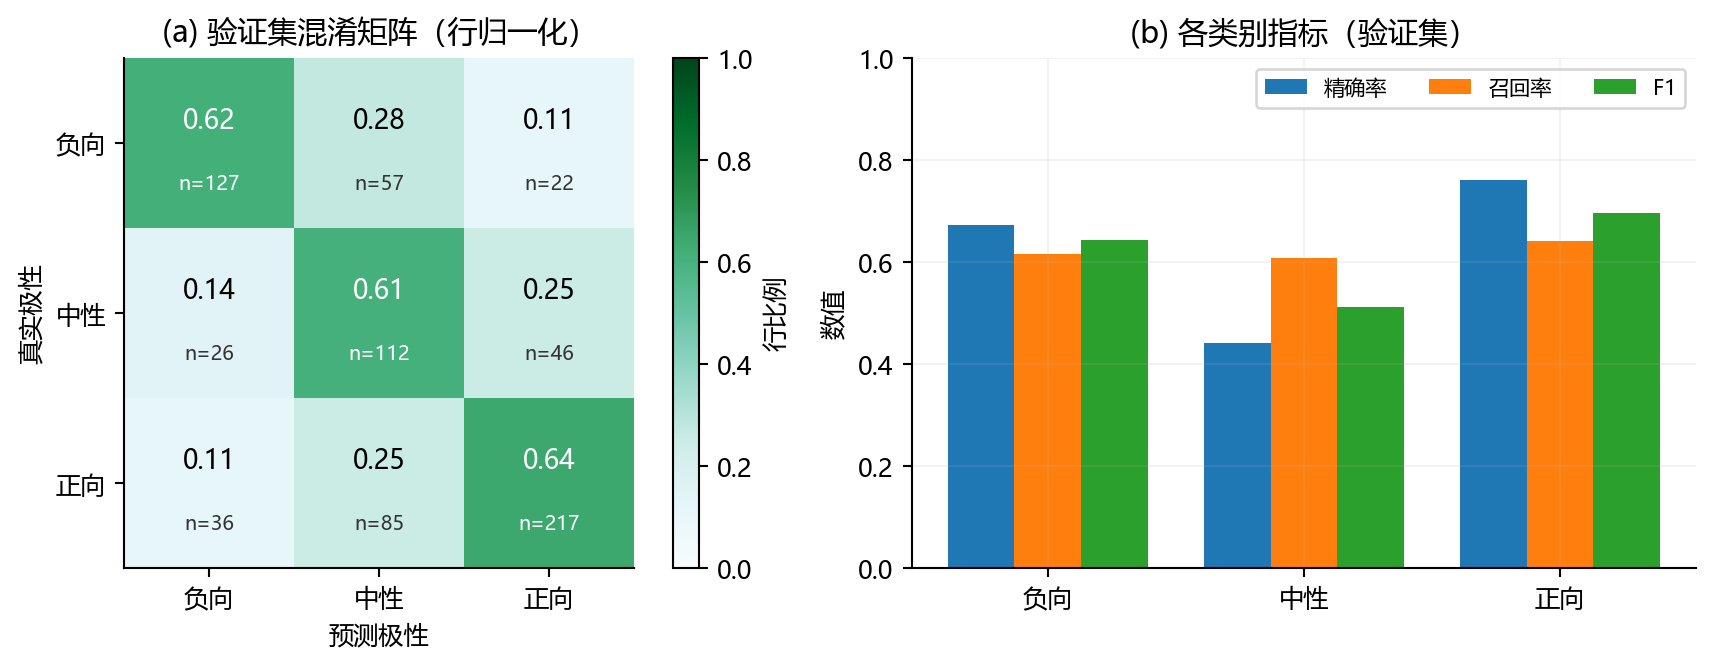
\includegraphics[width=.92\linewidth]{figures/q3_performance.png}
\caption{验证集混淆矩阵与分类指标}\label{q3:fig:perf}\end{figure}

表\ref{q3:tab:ablation}进一步比较子集训练、网络容量及一致性约束的影响。评价同时考虑预测指标、局部解释响应与种子间主模态一致性，以观察不同方案的收益与代价。

\begin{table}[H]\centering\small
\caption{候选方案与实现对照的验证结果}\label{q3:tab:ablation}
\begin{tabular}{lrrrrrr}\toprule
& \multicolumn{4}{c}{预测指标} & \multicolumn{2}{c}{解释指标}\\
\cmidrule(lr){2-5}\cmidrule(lr){6-7}
方案 & $J$ & Macro-F1 & MAE & 缺失平均F1 & AOPC差 & 种子一致率\\\midrule
仅完整输入（单种子） & 0.5470 & 0.6073 & 0.6030 & --- & --- & --- \\
无内容区打包对照 & 0.5468 & 0.6073 & 0.6048 & --- & --- & --- \\
\textbf{C0：子集训练} & \textbf{0.5575} & \textbf{0.6170} & \textbf{0.5954} & \textbf{0.4622} & \textbf{0.1068} & \textbf{84.0\%} \\
V1：采样与遮挡 & 0.5525 & 0.6112 & 0.5869 & 0.4368 & 0.1300 & 77.8\% \\
V2：增加容量 & 0.5527 & 0.6128 & 0.6010 & 0.4835 & 0.1119 & 79.2\% \\
V3：单调正则 & 0.5591 & 0.6192 & 0.6011 & 0.4421 & 0.1241 & 75.7\% \\
\bottomrule\end{tabular}\end{table}
V3的$J$略高于C0，但其缺失平均F1低于C0并超出容差，种子一致率也明显下降，预测与解释指标并未同步改善；V2的缺失平均F1最高，但$J$低于容差下界；V1的两项预测指标同时低于门槛。三者的解释AOPC差均达到门槛，据此选择C0作为最终SAP预测器，后续贡献分解和附件4推理均使用该模型。表中加粗行为最终选用配置，缺失平均F1为去文本、去语音、去视觉与全缺失四种状态下Macro-F1的平均值；仅完整输入对照采用单种子，其余方案采用三种子集成，种子一致率指主要参考模态的两两一致率平均值。

C0去掉文本后的Macro-F1降至0.4150，去语音与去视觉后的下降都有限，文本删除造成的下降最大，与联盟分解中文本主导的结论一致。仅用完整输入训练的单种子模型去文本后下降更深，两者集成规模不同，该差值同时包含训练方案与集成的影响。全缺失条件仅用于输入状态诊断，其预测仍可利用保留的内容长度。

\FloatBarrier
\paragraph{时序汇聚改进实验}
为增强不同位置的区分能力，在同一C0训练方案下，将均值汇聚替换为可学习的时序加权汇聚，保留最大池化，评分层零初始化。替换后强度误差下降而分类指标退化，未通过预设门槛。三个种子集成后，强度误差有所降低，但Macro-F1下降，$J$未达到预设的改善要求；候选未通过预测条件，因此不进入开发子集解释指标的比较，最终预测器保持C0，时序权重不用于替代干预解释。

\FloatBarrier
\paragraph{模态作用差异}
三模态平均Shapley贡献中，文本为$+1.105$，语音与视觉合计不足其十分之一；96条子集中分类主参考模态为文本86条，其余10条由语音或视觉主导，主导地位在样本层面并非绝对。
图\ref{q3:fig:coal}给出模态联盟的平均分类价值与三模态平均Shapley贡献：文本构成预测的主导信息来源，语音与视觉在三模态协同中提供补充信息，主参考模态分布与贡献排序一致。样本层的正负贡献与主参考模态另行保留，以刻画个体差异。
\begin{figure}[H]\centering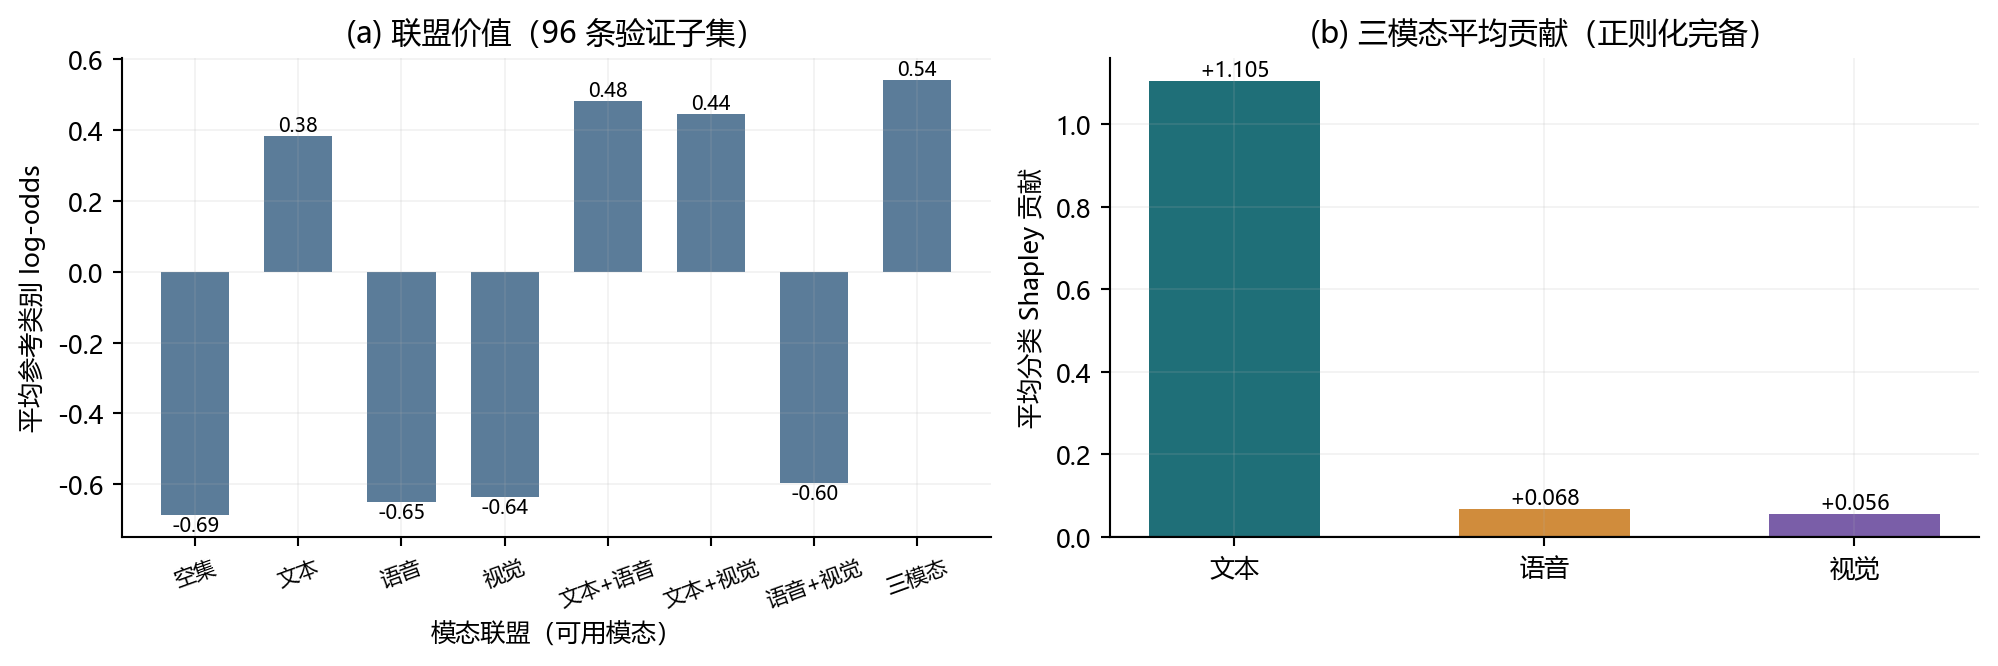
\includegraphics[width=.94\linewidth]{figures/q3_coalition_value.png}
\caption{模态联盟的平均分类价值与三模态平均Shapley贡献}\label{q3:fig:coal}\end{figure}

\FloatBarrier
\paragraph{局部证据与解释检验}
验证样本的局部块干预中，文本、语音与视觉的平均绝对log-odds响应分别为0.377、0.015与0.025，文本高出语音与视觉一个数量级以上。方向构成上，文本与语音的多数块支持参考类别，视觉块支持与抑制的比例接近；按句首、句中、句尾分段，文本的三段平均响应量级接近，局部证据没有集中在序列的固定位置。典型样本的逐块分布见图\ref{q3:fig:cardturn}。本段统计对应开发阶段的验证子集，冻结测试子集的双任务结果在下文单独分析。

逐档累计删除时，高分片段引起的参考类别概率下降明显大于随机片段，低分片段的影响接近于零；高分片段相对随机片段的AOPC配对差为0.1068，区间不含零。三类片段的曲线随删除档位单调展开，排序优势在整个档位区间内保持，实际锚点覆盖率随档位上升，区间描述该验证子集上的配对差异。

在最高删除档位，条件充分性仍存在偏差，说明主要模态中的剩余片段仍参与预测。沿用分类证据排序观察回归响应，删除高分块时强度的绝对变化明显大于删除低分块，表明分类关键片段也会影响连续强度输出。分类与回归的模态贡献分别计算，附件4有5条样本的两个任务主模态不同。

在主模态为文本的样本中，按自定义词表判定，最高分证据块完全由功能词或标点构成的比例低于全部文本块的平均水平，证据排序并未落在无实义的词上。

\FloatBarrier
\paragraph{冻结模型后的双任务确认}
选模完成后，以固定随机种子20261001从附件2测试集抽取96条样本，覆盖85个原视频。模型与解释规则保持冻结；按原视频聚类进行2000次配对bootstrap，保留同源片段之间的相关性。该子集未参与本次候选选择，但历史测试集已有评估记录。

如图\ref{q3:fig:faith}左、中两幅所示，分类与强度任务的高分块曲线在三个删除档位均高于随机块曲线，说明各自的排序均能定位影响输出的片段。分类高分块相对随机块的平均概率降幅差为0.1318，区间不含零；强度任务单独确定主模态与片段排序，其绝对预测变化差同样为正且区间不含零。两类曲线分别衡量参考类别概率与连续强度的响应，不等同于相对真实标签的误差变化；强度条件充分性在最高档位仍有偏差，说明少量关键片段尚不能完整复现原预测。

图\ref{q3:fig:faith}右图同时比较总体一致率与Cohen $\kappa$。在该确认子集上，B1与B2的主模态一致率较高、$\kappa$为中等水平；B1与B3的总体一致率同样较高，但$\kappa$接近于零。局部片段删除具有稳定的平均响应优势，主模态归因则依赖解释基线，尤其是少数非文本主导样本。

\begin{figure}[H]\centering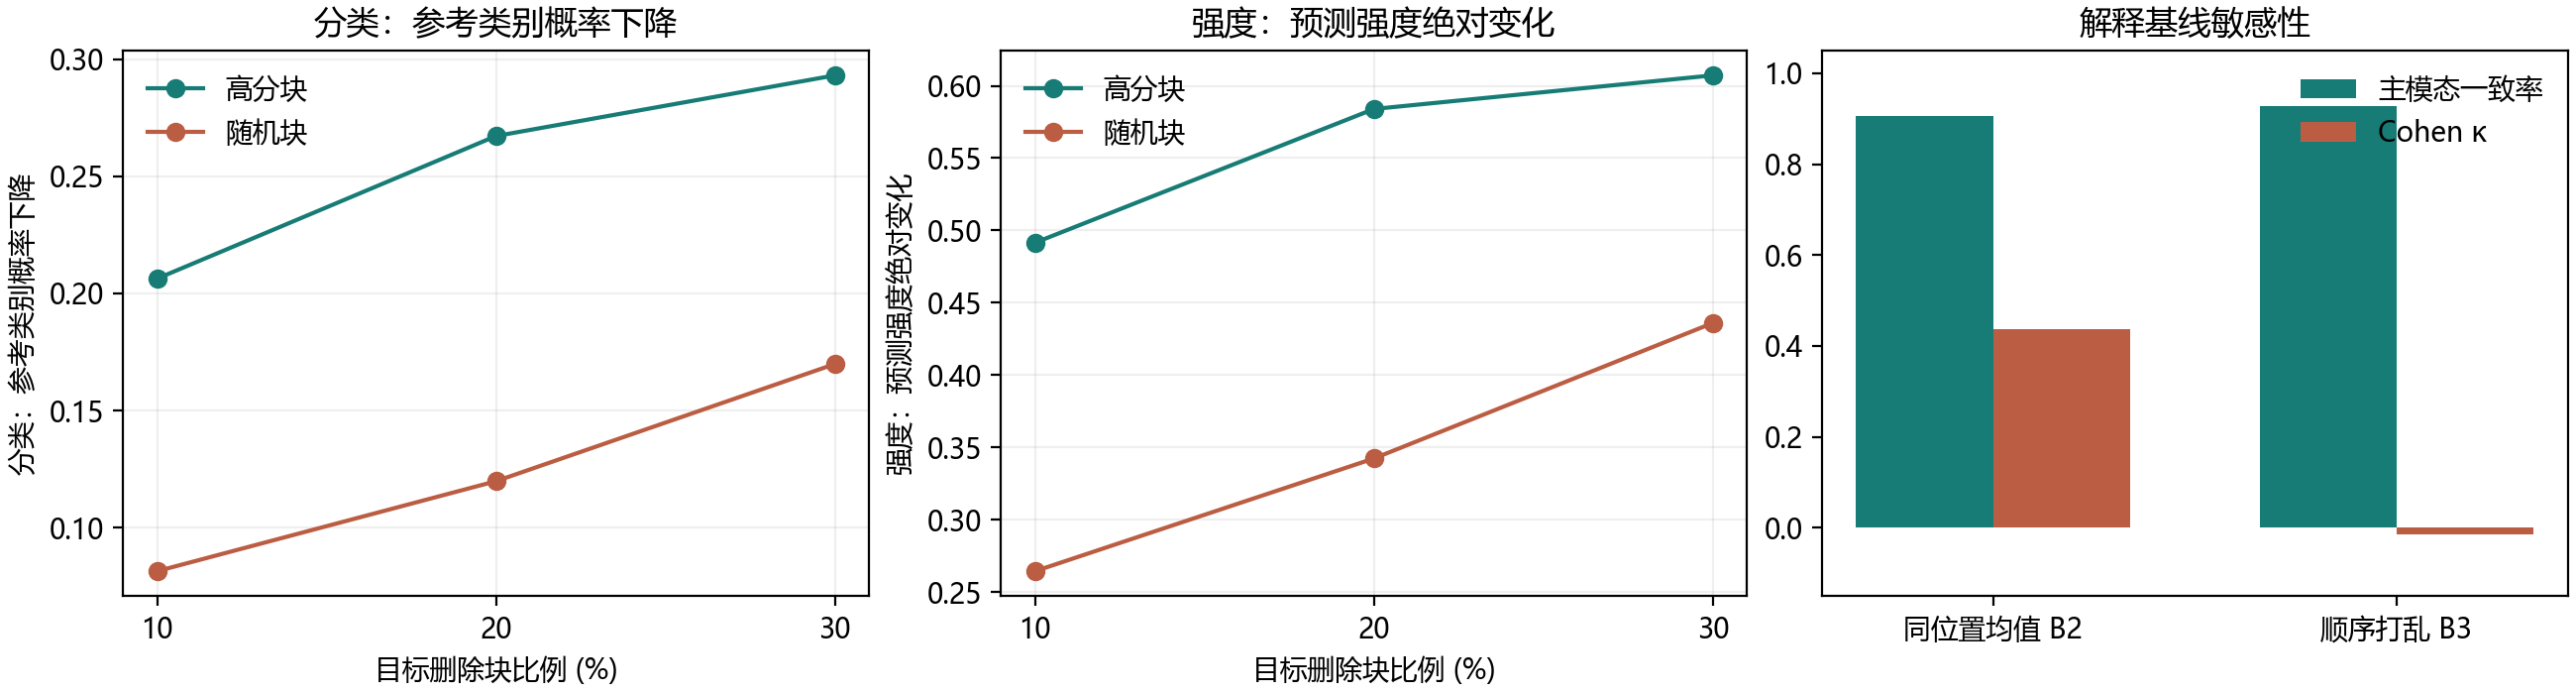
\includegraphics[width=\linewidth]{figures/q3_confirmation.png}
\caption{冻结测试子集上的分类与强度删除验证及解释基线敏感性}\label{q3:fig:faith}\end{figure}

\FloatBarrier
\paragraph{解释稳定性}
\textbf{总体上的文本主导结论稳定，少数非文本归因对基线选择敏感。}表\ref{q3:tab:stability}同时报告主模态一致率与Cohen $\kappa$，以区分总体一致程度和主模态分布偏斜的影响。验证子集中B1与B2的主模态一致率较高、$\kappa=0.5686$；B1与B3的一致率略低，$\kappa$降至$-0.0231$，B1下由语音或视觉主导的样本在B3下全部转为文本。两种基线下的绝对贡献排序保持中高度正相关。
\begin{table}[H]\centering\small
\caption{主参考模态与贡献排序在不同种子和解释基线下的一致性}\label{q3:tab:stability}
\begin{tabular}{llrrr}\toprule
样本范围 & 比较对象 & 一致率(\%) & Cohen $\kappa$ & 贡献排序相关\\\midrule
验证子集96条 & 种子0与1 & 82.29 & 0.2402 & ---\\
验证子集96条 & 种子0与2 & 83.33 & 0.1768 & ---\\
验证子集96条 & 种子1与2 & 86.46 & 0.2244 & ---\\\midrule
验证子集96条 & B1与B2 & 90.62 & 0.5686 & 0.812\\
验证子集96条 & B1与B3 & 87.50 & -0.0231 & 0.625\\\midrule
附件4全部20条 & B1与B2 & 75.00 & -0.0753 & 0.725\\
\bottomrule\end{tabular}\end{table}
三个训练种子的两两一致率处于同一水平，对应$\kappa$偏低，反映主模态分布高度不平衡；附件4在B1与B2下有个别样本改变主模态，贡献排序相关仍为正，其解释应结合具体基线与局部片段共同阅读。表中贡献排序相关为绝对贡献排序的Spearman相关系数，种子之间只统计主模态一致率。

\FloatBarrier
\paragraph{错误分布与归因分析}
验证集误判中有78.7\%涉及中性；按真实分组看，弱情感组（非中性且强度接近零点）的错误率最高，中性组次之，强情感组最低，说明零点附近的类别判别比强情感的方向判断更困难。错误分析将改进重点指向中性边界与弱情感区间的表征增强。

在96条解释样本中，低强度组的解释不稳定率略高于高强度组，两组都覆盖正确与错误预测样本；三种子最大类概率的标准差在两组间差异不显著，预测不确定性未随强度幅值系统变化。

\FloatBarrier
\paragraph{附件4全量结果}
全部20条样本的预测为中性7条、负向7条、正向6条，分类主参考模态为文本19条、视觉1条。图\ref{q3:fig:a4}从强度分布、分类模态份额和种子间波动三个角度展示全量结果；多数样本的文本份额较高，第8条以视觉为主，体现个体差异。第13条的视觉分支不可用，其视觉份额标记为NA，其余两个模态照常给出贡献。附件4中有2条样本的预测极性与强度符号相反：4-04为负向、强度$+0.089$，4-19为负向、强度$+0.188$，类别与强度由两个独立输出头给出，符号可以不同；该分歧集中在强度接近中性的位置：附件2测试集方向明确的513条样本中，两任务方向一致的有503条（98.05\%）；10条不一致样本的强度绝对值全部不超过$1/3$，其中7条低于$0.2$，而方向明确样本中$|r|<0.2$的仅占3.3\%。

跨模态核查中，多数样本的全部可用模态最高分证据均指向预测类别，个别反向项均来自视觉分支且幅度远小于文本主证据，判别主体仍落在文本证据上。按与验证集相同的删除协议，附件4样本上高分块相对随机块的平均概率下降差为0.1316，区间不含零，逐块响应在无标签样本上同样稳定区分证据块与随机块。
\begin{figure}[H]\centering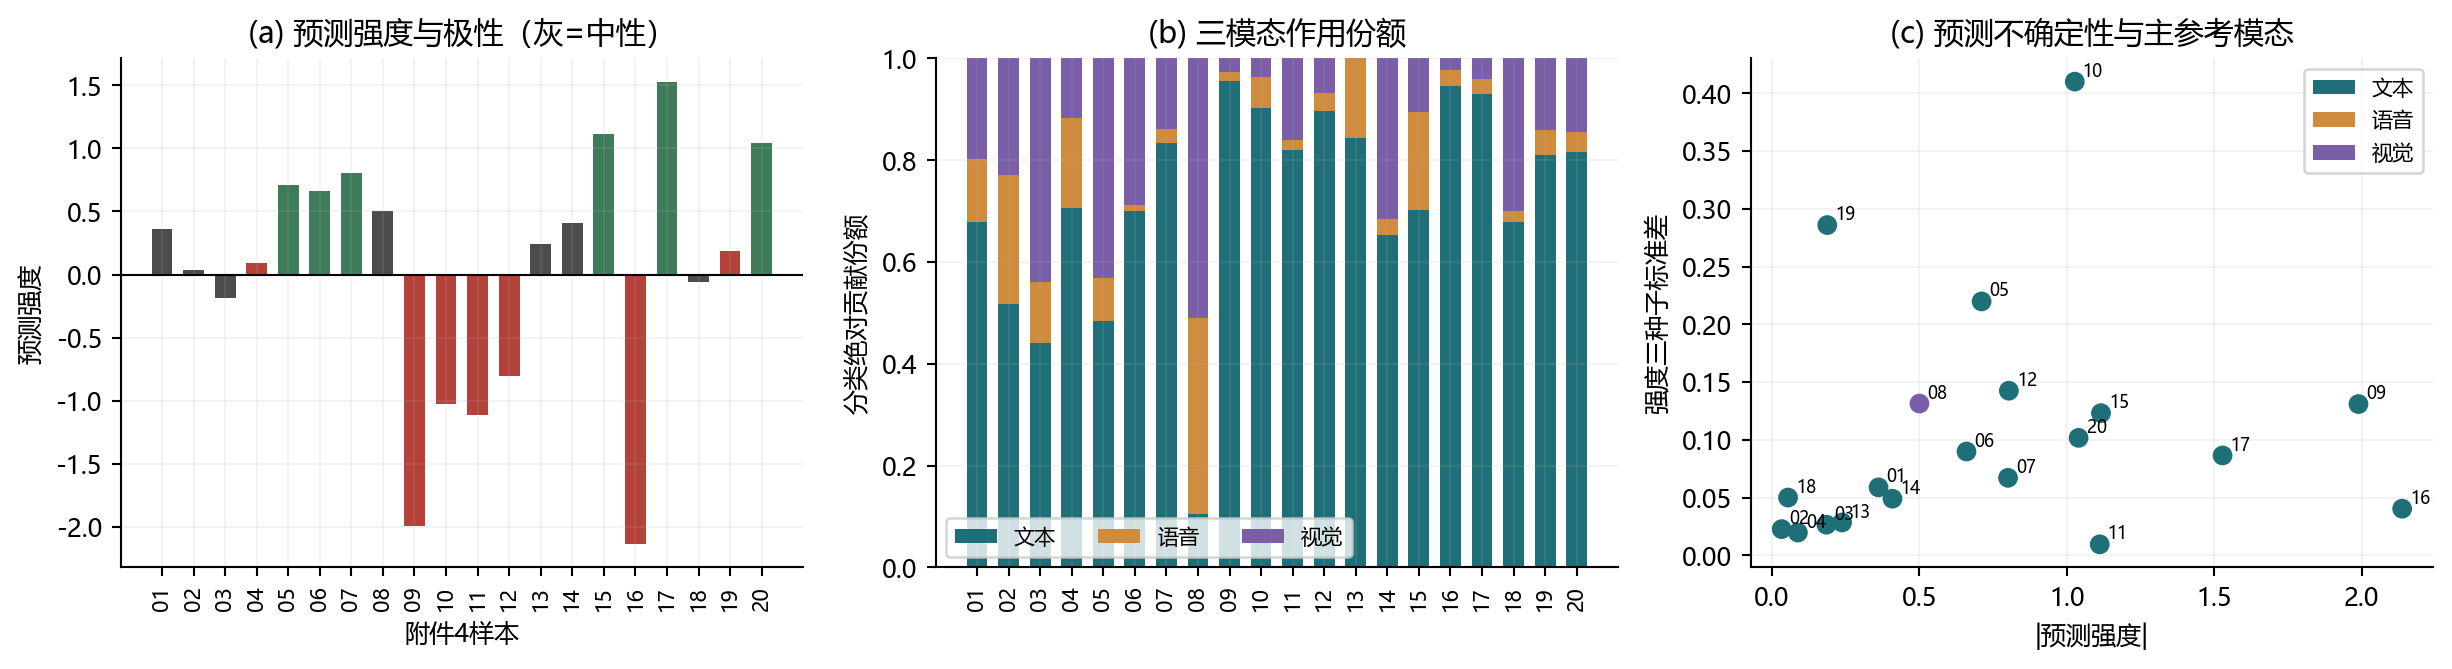
\includegraphics[width=\linewidth]{figures/q3_a4_overview.png}
\caption{附件4全部20条样本的情感预测、模态作用份额与种子间波动}\label{q3:fig:a4}\end{figure}
表\ref{q3:tab:all20}列出逐条预测及作用份额，便于与图\ref{q3:fig:a4}核对。其中NA表示输入特征不可用，不能解释为该模态贡献为零；分类极性与连续强度分别来自两个输出头。

\begingroup\small
\begin{longtable}{clrrrrl}
\caption{附件4全量预测与分类模态作用份额}\label{q3:tab:all20}\\
\toprule
编号 & 极性 & 强度 & 文本份额 & 语音份额 & 视觉份额 & 主模态\\\midrule
\endfirsthead
\caption*{续表\ \thetable}\\
\toprule
编号 & 极性 & 强度 & 文本份额 & 语音份额 & 视觉份额 & 主模态\\\midrule
\endhead
\bottomrule
\endlastfoot
4-01 & 中性 & +0.362 & 0.678 & 0.124 & 0.198 & 文本 \\
4-02 & 中性 & +0.034 & 0.518 & 0.254 & 0.229 & 文本 \\
4-03 & 中性 & -0.185 & 0.441 & 0.119 & 0.440 & 文本 \\
4-04 & 负向 & +0.089 & 0.705 & 0.178 & 0.116 & 文本 \\
4-05 & 正向 & +0.711 & 0.484 & 0.085 & 0.432 & 文本 \\
4-06 & 正向 & +0.660 & 0.699 & 0.014 & 0.287 & 文本 \\
4-07 & 正向 & +0.801 & 0.833 & 0.029 & 0.138 & 文本 \\
4-08 & 中性 & +0.501 & 0.106 & 0.384 & 0.510 & 视觉 \\
4-09 & 负向 & -1.989 & 0.955 & 0.018 & 0.027 & 文本 \\
4-10 & 负向 & -1.027 & 0.903 & 0.060 & 0.037 & 文本 \\
4-11 & 负向 & -1.112 & 0.820 & 0.020 & 0.160 & 文本 \\
4-12 & 负向 & -0.804 & 0.897 & 0.036 & 0.067 & 文本 \\
4-13 & 中性 & +0.238 & 0.844 & 0.156 & NA & 文本 \\
4-14 & 中性 & +0.409 & 0.654 & 0.031 & 0.315 & 文本 \\
4-15 & 正向 & +1.116 & 0.703 & 0.192 & 0.105 & 文本 \\
4-16 & 负向 & -2.137 & 0.946 & 0.031 & 0.022 & 文本 \\
4-17 & 正向 & +1.528 & 0.930 & 0.029 & 0.040 & 文本 \\
4-18 & 中性 & -0.055 & 0.679 & 0.021 & 0.300 & 文本 \\
4-19 & 负向 & +0.188 & 0.809 & 0.049 & 0.141 & 文本 \\
4-20 & 正向 & +1.040 & 0.816 & 0.040 & 0.144 & 文本 \\
\end{longtable}
\endgroup
\FloatBarrier
\paragraph{典型样本与证据回映}
解释卡把预测结论、模态份额、证据词时间与原始素材组织在同一视图中，用于检验模型响应与可观察线索的对应关系。附件4第12条的预测为负向（最大类概率0.76，强度$-0.804$），主要参考模态为文本（份额0.897）：原文前段为\textit{previously had good credit}，转折词\textit{but}（3.88\,s）之后转入信用下滑的负面叙述，最高分证据片段为\textit{sag,}（9.94--10.30\,s），同时是语音的最高分证据块，两个模态的证据落在同一词上。沿用问题一的韵律度量，\textit{but}处音高相对前段抬高2.3半音、能量抬升0.88，证据词处音高抬高2.3半音、能量抬升0.52，构成样本内两处局部韵律突起点；卡片中的全段韵律轨迹给出能量与音高随时间的走向。图\ref{q3:fig:cardturn}中黄底标记主要模态的最高分证据词，蓝底标记其他模态的最高分证据词，卡片同时给出全段韵律轨迹、语音证据片段与逐块响应。
\begin{figure}[H]\centering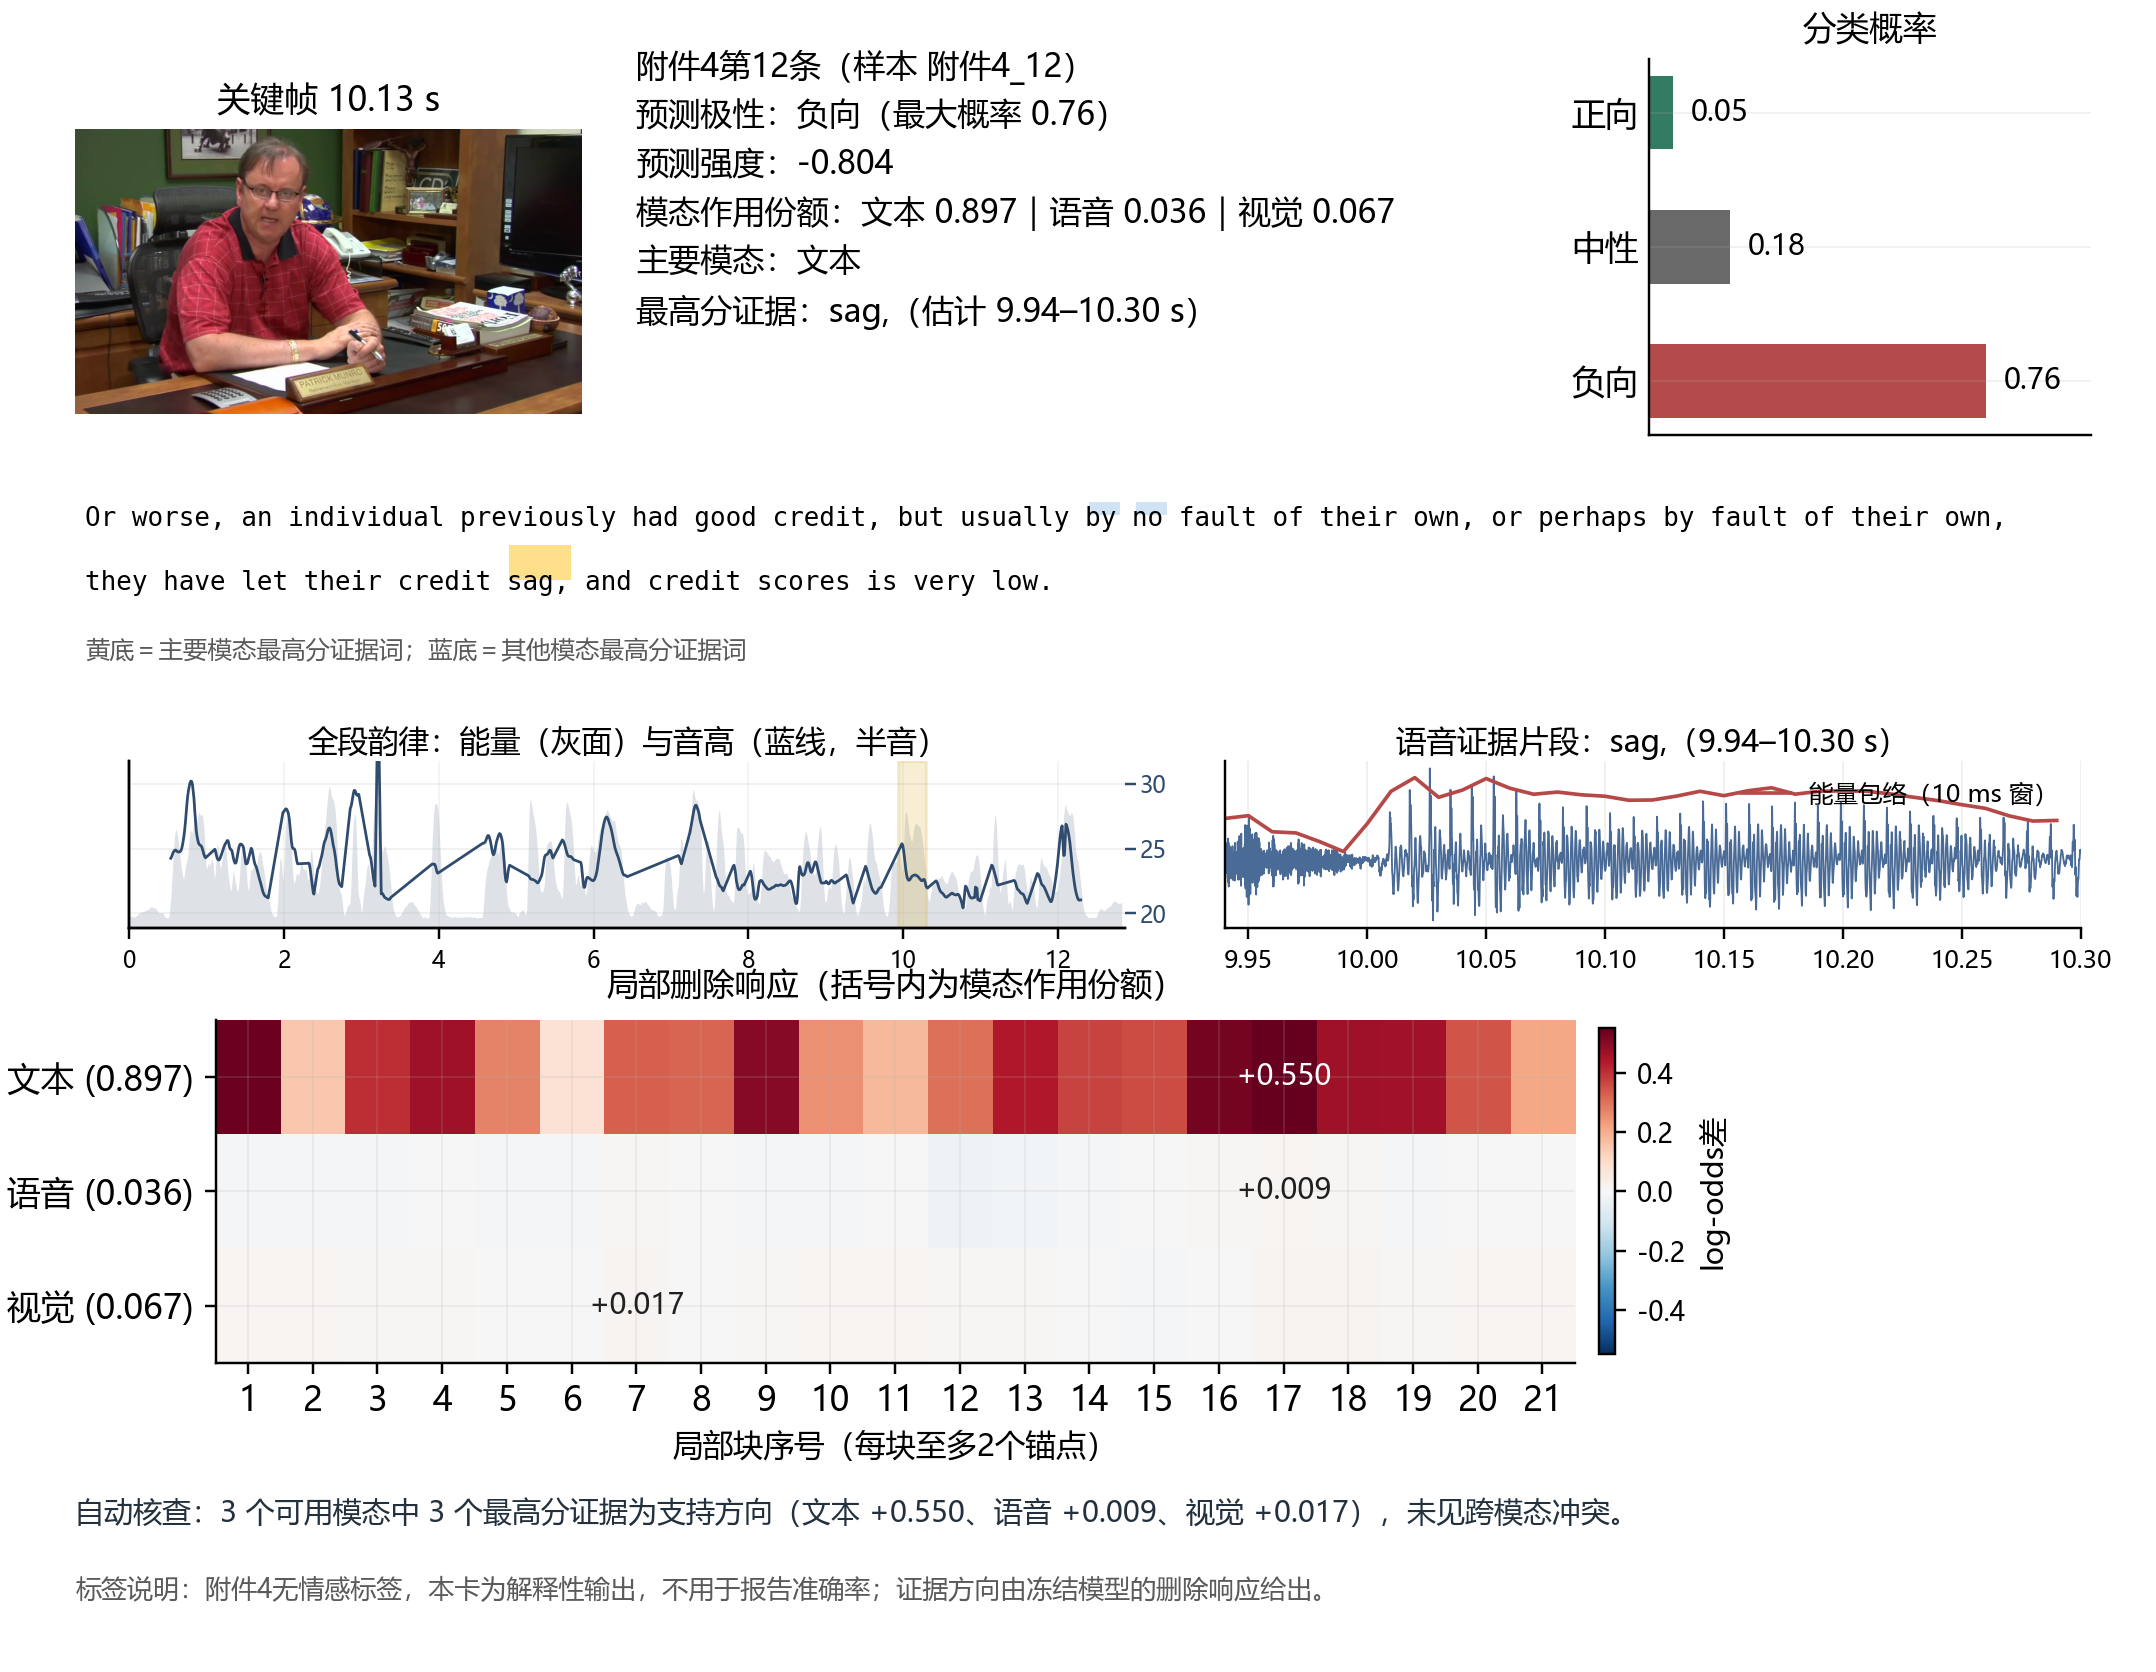
\includegraphics[width=\linewidth]{figures/q3_card_12.png}
\caption{附件4第12条（转折样本）解释卡}\label{q3:fig:cardturn}\end{figure}
20条样本的重新分词序列均与官方词元一致，482个原词中478个获得CTC时间区间；该回映与问题一共用同一套对齐实现，词表构建与CTC强制对齐直接调用问题一的模块，问题一建立的词元—锚点—时间对应关系由此成为后两问共享的时序基础。新增双任务证据共120条，其中118条可用记录均完成时间回映并导出音频与关键帧；其余2条为第13条样本的视觉特征不可用，在分类与强度任务中分别标记NA。每条记录保存原素材哈希、词元锚点、作用方向、时间区间及真实帧PTS，构成从模型响应到原素材的可追溯链条。

本模型把情感预测分解为可复核的模态贡献与局部响应，并通过词级时间区间连接到原始素材：Shapley值度量指定模型与基线下的作用差异，删除实验检验局部证据与预测响应的一致性。两项分析在同一预测器上完成，因此解释结论可直接对应该模型的决策过程。
\FloatBarrier

\section{模型检验与灵敏度分析}
\subsection{模型检验}
模型检验分别围绕时间对应、缺失预测与解释忠实性展开。

问题一中，100条样本均形成输出，1920个已生成词区间全部满足非负起点、正长度、音轨范围内终点与起点随词序单调四项约束。典型样本展示了词元、声学窗口与视频帧的对应关系，6条超长样本保留完整词级记录，定长接口截断不影响样本覆盖。

问题二中，验证集Macro-F1为0.6163、强度MAE为0.5818。273条分类错误中，213条涉及中性类，占78.0\%。测试集使用共用掩码，将七类输入处理与结构基线和两个公开基线与本文模型置于同一协议下比较。经来源视频分组配对bootstrap及Holm校正，18项局部比较中，相对模态丢弃的局部F1差异以及相对均值填充、三态嵌入、LMF、MulT的局部MAE差异达到5\%显著性水平。

问题三中，模态Shapley分解的效率残差不超过$8.9\times10^{-16}$，满足效率性公理。在96条验证子集上，高分片段删除相对随机删除的AOPC差为0.1068，95\%区间为[0.0887,0.1259]，说明局部响应排序与预测变化相符。该检验评价解释对当前模型的忠实性，主模态对基线与随机种子的敏感性另见表\ref{q3:tab:stability}。

\subsection{灵敏度分析}
时间对齐模型的灵敏度主要来自词边界与聚合参数。所选12条样本子集中，扰动次数由50增至200后，视觉方差的排序相关为0.995，锚点相对排序较为稳定。边界扰动尺度由40\,ms改为20或80\,ms时，音视频质量分数的排序相关均在0.90以上，说明该质量评价在所测范围内具有较好的排序一致性。

局部缺失预测的灵敏度从模态组合、连续区间比例、位置和长度四个方面检验。三模态居中缺口的目标长度由1增至16个锚点时，F1由0.6047变为0.4632，MAE由0.6496变为0.7981。逐样本对照显示，三模态共缺20\%（居中缺口）时60条样本由正确变为错误、48条由错误变为正确，16个锚点缺口下缺失时的分类错误中有50.1\%在完整输入下本已错误。短样本按$L_i-1$截断，并另报告各条件均满足局部删除与保留观测要求的共同子集，区分缺失程度变化与样本边界效应。

解释模型的灵敏度表现为少数样本的主模态变化。B1与B2在验证子集上的$\kappa$为0.5686，B1与B3为$-0.0231$；B3下原有10条非文本主导样本均转为文本。文本在总体上占主导，而非文本贡献需要结合解释基线考察。

\section{模型评价与推广}
\subsection{模型特点}
\textbf{时间组织明确。} 以原词区间连接子词表示与音视频帧，用交叠权重统一不同采样粒度，并以观测掩码保留缺失状态，形成从定长特征到原始素材的对应关系。

\textbf{缺失处理与任务学习相结合。} 三态输入区分结构填充、有效观测和局部缺失，补全表示通过门控参与融合，EMT-DLFR教师提供分类与强度软监督。局部输入模态消融及连续缺口实验分别刻画模态敏感性与缺失程度的影响。

\textbf{解释对应同一预测器。} 模态联盟分解与局部删除共享预测模型，分别给出模态贡献和片段响应，再通过词级时间映射定位原始证据，使预测数值与解释结果相互对应。

\subsection{模型局限与改进}
时间对齐采用自动估计的词区间，当前验证侧重覆盖、结构与相对时序一致性。可进一步加入人工词边界标注，评价起止点误差，并改善数字读法与长序列处理。

缺失预测的分类误差集中于中性与非中性类别之间，逆频率加权均衡了训练目标中的类别贡献，但类别识别仍取决于样本的有效证据。后续可加强缺口上下文与弱情感样本的区分，通过组件消融和独立数据进一步检验补全、蒸馏的作用。

解释结果随基线和训练种子变化，非文本主导样本尤为明显。新增冻结测试子集分别确认了分类与强度片段的删除响应，双任务证据均已回映至原素材；进一步改进可结合独立数据与人工时间标注，检验解释迁移性及定位误差。

在应用推广中，词级锚点与掩码表示可用于其他具有转写文本的音视频分析任务；模型结构和参数需结合新任务的特征维度、缺失模式与标签分布重新确定。

\section{结论}
本文围绕多模态情感预测的时间组织、局部缺失与决策解释，建立三个相互关联的模型，主要结论如下。

第一，以原词为公共时间锚点，通过CTC强制对齐、子词归属与时间交叠池化，完成附件1全部100条样本的三模态特征提取。1932个原词中1920个生成时间区间，生成率99.38\%；全量结果表、观测掩码与典型片段给出特征与原始素材的对应关系，质量分量与边界扰动记录进一步刻画各锚点的可用程度，该时间表示为缺失掩码与证据回映提供了统一定义。

第二，采用EMT-DLFR教师与逆频率类别加权的三态感知学生模型，在验证集上取得0.6163的Macro-F1和0.5818的强度MAE，并完成附件3全部30条样本的预测。测试集基础Macro-F1为0.6189、MAE为0.6221；105种连续局部缺失条件下的平均Macro-F1为0.6066、MAE为0.6492。目标区间比例由5\%增至40\%时F1累计下降0.0240，缺口位置带来的平均差异为0.0090，缺口越重相对通用融合框架的优势越大，模型在局部缺失下保持稳定输出，性能损失集中在覆盖样本主体的文本长缺口上。

第三，模态子集训练与输入干预相结合的解释模型完成附件4全部20条样本的预测与解释，输出中性7条、负向7条、正向6条。冻结测试子集上分类与强度任务的高分片段删除优势分别为0.1318和0.2132，两种任务的局部排序均能定位影响当前输出的片段；118条可用证据完成时间与媒体回映，文本贡献总体占主导，少数非文本归因对解释基线较为敏感。

上述模型分别给出统一的时间表示、面向局部缺失的预测方式与对应模型决策的证据定位，形成从原始素材到预测与解释的可追溯链条。其结构不依赖特定数据集，可按新任务的特征维度、缺失模式与标签分布重新配置，用于具有转写文本的音视频情感分析场景。

\addcontentsline{toc}{section}{参考文献}
\begin{thebibliography}{99}
\bibitem{ref:mm} Baltrusaitis T, Ahuja C, Morency L P. Multimodal machine learning: A survey and taxonomy[J]. IEEE Transactions on Pattern Analysis and Machine Intelligence, 2019, 41(2): 423--443.
\bibitem{ref:mosei} Zadeh A, Liang P P, Poria S, Cambria E, Morency L P. Multimodal language analysis in the wild: CMU-MOSEI dataset and interpretable dynamic fusion graph[C]. Proceedings of the 56th Annual Meeting of the Association for Computational Linguistics (ACL), 2018: 2236--2246.
\bibitem{ref:tfn} Zadeh A, Chen M, Poria S, Cambria E, Morency L P. Tensor fusion network for multimodal sentiment analysis[C]. Proceedings of the 2017 Conference on Empirical Methods in Natural Language Processing (EMNLP), 2017: 1103--1114.
\bibitem{ref:mtfn} Tsai Y H H, Bai S, Liang P P, Kolter J Z, Morency L P, Salakhutdinov R. Multimodal transformer for unaligned multimodal language sequences[C]. Proceedings of the 57th Annual Meeting of the Association for Computational Linguistics (ACL), 2019: 6558--6569.
\bibitem{ref:bert} Devlin J, Chang M W, Lee K, Toutanova K. BERT: Pre-training of deep bidirectional transformers for language understanding[C]. Proceedings of the 2019 Conference of the North American Chapter of the Association for Computational Linguistics (NAACL-HLT), 2019: 4171--4186.
\bibitem{ref:wav2vec2} Baevski A, Zhou Y, Mohamed A, Auli M. wav2vec 2.0: A framework for self-supervised learning of speech representations[C]. Advances in Neural Information Processing Systems (NeurIPS), 2020: 12449--12460.
\bibitem{ref:ctc} Graves A, Fernandez S, Gomez F, Schmidhuber J. Connectionist temporal classification: Labelling unsegmented sequence data with recurrent neural networks[C]. Proceedings of the 23rd International Conference on Machine Learning (ICML), 2006: 369--376.
\bibitem{ref:kd} Hinton G, Vinyals O, Dean J. Distilling the knowledge in a neural network[EB/OL]. arXiv:1503.02531, 2015.
\bibitem{ref:emt} Sun L, Lian Z, Liu B, Tao J. Efficient multimodal transformer with dual-level feature restoration for robust multimodal sentiment analysis[J]. IEEE Transactions on Affective Computing, 2023.
\bibitem{ref:lmf} Liu Z, Shen Y, Lakshminarasimhan V B, Liang P P, Zadeh A, Morency L P. Efficient low-rank multimodal fusion with modality-specific factors[C]. Proceedings of the 56th Annual Meeting of the Association for Computational Linguistics, 2018: 2247--2256.
\bibitem{ref:shapley} Shapley L S. A value for n-person games[M]//Kuhn H W, Tucker A W. Contributions to the Theory of Games II. Princeton: Princeton University Press, 1953: 307--317.
\bibitem{ref:lime} Ribeiro M T, Singh S, Guestrin C. "Why should I trust you?": Explaining the predictions of any classifier[C]. Proceedings of the 22nd ACM SIGKDD International Conference on Knowledge Discovery and Data Mining (KDD), 2016: 1135--1144.
\bibitem{ref:shap} Lundberg S M, Lee S I. A unified approach to interpreting model predictions[C]. Advances in Neural Information Processing Systems (NeurIPS), 2017: 4765--4774.
\end{thebibliography}

\appendicesbegin
\phantomsection
\addcontentsline{toc}{section}{附录}
\addtocontents{toc}{\protect\setcounter{tocdepth}{-1}}
\section{问题一自生成特征文件的存储组织}
\label{app:q1-files}

表\ref{q1:tab:checklist}所列张量、逐样本记录、帧级支撑与逐词明细构成问题一的全量特征文件，随附件提交；运行环境、关键参数、逐阶段耗时与输入哈希由程序在运行时自动记录，复现记录一并随支撑材料提交。特征张量、词级时间与帧级记录以样本键关联：读取时由样本键定位逐样本记录，再按内容掩码$P$与父词索引$U$将接口位置还原到词级区间。存储格式、组织结构与读取方式见表\ref{q1:tab:checklist}。

\begin{table}[htbp]
\centering\small
\caption{自生成特征文件的存储组织与读取方式}
\label{q1:tab:checklist}
\begin{tabularx}{\linewidth}{>{\raggedright\arraybackslash}p{5.1cm}Y}
\toprule
文件 & 内容与读取方式 \\
\midrule
\file{E1\_features.pkl} & 全部100条样本的$X^t/X^a/X^v$、掩码与质量分量的汇总字典，含版本号与样本数；按样本键索引，用于全量读取与跨样本统计 \\
\file{per\_sample/} & 逐样本记录，含特征矩阵、内容掩码$P$、父词索引$U$、观测掩码$O^a/O^v$、词级记录与元数据；文件名由样本键转换得到，是逐样本核对与追溯的入口 \\
\file{frames/} & 帧级支撑，含音频帧特征与起止区间、视频帧PTS与有效标记；与逐样本记录按同一键关联，是帧级时间与覆盖的来源 \\
\file{E1\_alignment\_detail.csv} & 1932条逐词明细，含区间$[a,b)$、路径置信度与覆盖、扰动及质量分量；用于定位单个词的时间与质量 \\
\file{E1\_manifest.csv} & 样本级清单，含文本与媒体统计、模态覆盖、逐阶段耗时与输入哈希；用于覆盖统计与结果核验 \\
\file{audit\_anchor.json} & 边界位置核验记录，含邻近停顿的1125个词界、734个随机对照的偏差分布与起止点分组统计；用于核对词界与声学停顿的对应关系 \\
\file{env\_run\_start.json}、\file{run\_events.log}、\file{run\_log.json} & 运行环境快照（Python与各库版本、解码器与推理设备）、事件日志（启动、跳过、失败与汇总）与参数汇总（工具、关键参数、耗时与输入哈希）；用于复现核对 \\
\bottomrule
\end{tabularx}
\end{table}

\section{问题二结果文件与交付说明}
\label{app:q2-files}

附件3的完整预测按原始样本顺序导出为\file{pred\_附件3.csv}，逐条给出预测极性、连续强度、三类概率、内容锚点数与三模态缺失计数，并附强度预测的种子间标准差；三类概率的排序、极性判决与强度符号可直接由该文件复核。

附件2上的评价结果与核验记录同步保留：\file{metrics.csv}保存十类模型在基础输入与105种连续缺失条件下的逐条件、逐种子分类与回归指标；\file{paired\_comparison.csv}保存相对九类基线的配对bootstrap区间与Holm校正结果；\file{mask\_audit.json}逐条件记录内容位、人工缺口与观测删除的核验值；\file{protocol.json}保存训练与评价协议参数及21个检查点的SHA-256哈希；\file{checks.json}保存划分、掩码与推理设备的一致性检查结果。上述文件与模型权重、逐种子训练日志随支撑材料一并提交。

\section{问题二专项模型核心代码}
\label{app:q2-code}

问题二局部缺失情感预测专项模型（TSRF-D）的完整实现与训练脚本随支撑材料提交（\file{问题二实现}目录）。以下按三态投影、门控补全和联合损失节选核心代码，与正文式\eqref{q2:eq:total_loss}及相应结构对应；节选保留源文件中的循环与省略位置，便于与支撑材料逐行核对。

\begin{lstlisting}[language=Python,basicstyle=\ttfamily\footnotesize,breaklines=true]
# q2_model.py: tri-state projection (content / observed / missing)
def _states(self, P, O):
    s = torch.where(P, torch.full_like(P, 2, dtype=torch.long),
                    torch.zeros_like(P, dtype=torch.long))
    s = torch.where(P & O, torch.ones_like(s), s)
    return s

def _project(self, X, P, O, true_target=False):
    z = {}
    for mi, m in enumerate(MODS):
        st = torch.ones_like(P, dtype=torch.long) if true_target else self._states(P, O[m])
        base = self.e_mod[mi] + self.e_pos[: P.shape[1]]
        zz = self.proj[m](X[m]) + (self.e_state[st] if self.cfg.use_state_emb else 0.0) + base
        z[m] = zz if true_target else zz * P[..., None]
    return z
\end{lstlisting}

\begin{lstlisting}[language=Python,basicstyle=\ttfamily\footnotesize,breaklines=true]
# q2_model.py: gated completion with distance, position and continuity prior
def _complete(self, z, P, O):
    cfg = self.cfg
    B, K = P.shape
    dev = P.device
    d = cfg.d
    known = {m: (P & O[m]) for m in MODS}
    run = {m: _run_length(known[m]) for m in MODS}
    cand_mask = torch.stack([known[m] for m in MODS], dim=1)          # (B,3,K)
    cmat = cand_mask[:, None].expand(B, 3, 3, K).reshape(B, 3, 3 * K)
    n_cand = cmat.sum(dim=-1)
    empty = (n_cand == 0)
    key = torch.stack([self.k_proj(z[m]) for m in MODS], dim=1)
    val = torch.stack([self.v_proj(z[m]) for m in MODS], dim=1)
    kmat = key.reshape(B, 3 * K, d)
    vmat = val.reshape(B, 3 * K, d)
    q_base = self.e_pos[:K][None, None, :, :] + self.e_state[2][None, None, None, :]
    q = self.q_proj(q_base.expand(B, 3, K, d) + self.e_mod[None, :, None, :])
    qf = q.reshape(B, 3 * K, d)
    d2 = (qf.pow(2).sum(-1)[:, :, None] + kmat.pow(2).sum(-1)[:, None, :]
          - 2.0 * torch.bmm(qf, kmat.transpose(1, 2))) / d
    d2 = d2.clamp(min=0.0).reshape(B, 3, K, 3 * K)
    cost = d2 + cfg.lam_t * self.dt[None, None, :, :]
    cost = cost + (1.0 - cmat.float())[:, :, None, :] * 1e4
    if cfg.use_u_score:
        u = torch.stack([torch.sigmoid(cfg.alpha0 + cfg.alpha1 * known[m].float()
                                       + cfg.alpha2 * (run[m] / cfg.run_scale).clamp(0.0, 1.0))
                         for m in MODS], dim=1)
    else:
        u = torch.ones(B, 3, K, device=dev)
    cost = cost + cfg.lam_q * (1.0 - u.reshape(B, 3 * K))[:, None, None, :]
    cost = torch.where(empty[:, :, None, None], torch.zeros_like(cost), cost)
    pi = torch.softmax(-cost / cfg.temperature, dim=-1) * cmat.float()[:, :, None, :]
    pi = pi / pi.sum(-1, keepdim=True).clamp(min=1e-6)
    pi = torch.where(empty[:, :, None, None], torch.zeros_like(pi), pi)
    z_hat = torch.bmm(pi.reshape(B, 3 * K, 3 * K), vmat).reshape(B, 3, K, d)
    cost_rho = torch.where(cmat.bool()[:, :, None, :],
                           torch.clamp(cost, max=1e3),
                           torch.full_like(cost, 1e4))
    cbar = (pi * cost_rho).sum(-1)
    cvar = (pi * (cost_rho - cbar[..., None]).pow(2)).sum(-1)
    cmin = cost_rho.min(-1).values
    nsrc = (n_cand.float() / (3.0 * K))[:, :, None].expand(B, 3, K)
    aratio = torch.stack([known[m].float().sum(-1) / P.float().sum(-1).clamp(min=1)
                          for m in MODS], dim=1)[..., None].expand(B, 3, K)
    gin = torch.stack([cbar, cvar, cmin, nsrc, aratio], -1)          # (B,3,K,5)
    if cfg.use_target_mod_gate:
        gin = torch.cat([gin, self.e_mod[None, :, None, :].expand(B, 3, K, -1)], -1)
    rho = torch.sigmoid(self.g_rho(gin)).squeeze(-1)
    rho = torch.where(empty[:, :, None], torch.zeros_like(rho), rho)
    return z_hat, rho, dict(n_cand=n_cand, run=run)
\end{lstlisting}

\begin{lstlisting}[language=Python,basicstyle=\ttfamily\footnotesize,breaklines=true]
# q2_train.py: compute_loss (excerpt; num/cnt averaging kept from source)
l_cls = F.cross_entropy(logits, y, weight=batch["class_w"])
l_reg = F.huber_loss(r_hat, r, delta=1.0)
p = torch.softmax(logits, dim=-1)
l_cons = ((p[:, 2] - p[:, 0]) - torch.tanh(r_hat / 3.0)).pow(2).mean()
# ...
if cfg["use_rec"] and rec:
    num, cnt = 0.0, 0
    for m, d in rec.items():
        tgt = x_true[m][batch["hard"][m]]
        num = num + F.smooth_l1_loss(d["pred"], tgt, beta=1.0, reduction="mean")
        cnt += 1
    if cnt:
        l_rec = num / cnt
# ...
if cfg["use_kd_cls"] and batch.get("t_logits") is not None:
    T = float(cfg.get("T_kd", 2.0))
    tlog = batch["t_logits"].detach()
    pT = torch.softmax(tlog / T, dim=-1)
    logq = torch.log_softmax(logits / T, dim=-1)
    l_dc = F.kl_div(logq, pT, reduction="batchmean") * (T * T)
if cfg["use_kd_reg"] and batch.get("t_reg") is not None:
    l_dr = F.huber_loss(r_hat, batch["t_reg"].detach(), delta=1.0)
l = (l_cls + cfg["lam_r"] * l_reg + cfg["lam_c"] * l_cons
     + cfg["lam_dc"] * l_dc + cfg["lam_dr"] * l_dr
     + cfg["lam_rec"] * l_rec + cfg["lam_rel"] * l_rel)
\end{lstlisting}

\section{问题三结果文件与交付说明}
\label{app:q3-files}

附件4的预测、证据与逐块响应统一存放于交付目录\file{优化实验/输出}。\file{pred\_附件4.csv}保存全量预测及分类、强度双任务的有符号贡献；\file{evidence\_dual\_task.csv}按样本、模态与任务保存局部证据，共120行，逐条给出证据块的锚点位置、证据词、有符号响应、作用方向、CTC时间区间、关键帧索引与PTS、媒体文件及原视频哈希，其中118行完成时间回映，2行为第13条样本视觉分支不可用时的标记；\file{a4\_local\_all.json}保存全部逐块删除响应，可用于复核证据排序与作用方向。

解释卡按统一模板生成，保留有符号最高分片段、逐块响应、证据词时间与关键帧，涵盖跨模态分歧、视觉主模态与缺模态降级三类样本；逐样本的跨模态一致性记录见\file{cards\_summary.csv}，20张卡片与该表一并随支撑材料提交。特征可用性的核查记录见\file{audit\_a4.json}：逐样本统计三模态的缺失位数量，第13条视觉的30个内容位全零即由该记录标记，后续解释据此把该模态份额记为NA。

\section{问题三专项模型核心代码}
\label{app:q3-code}

问题三子集感知可解释预测专项模型的完整实现随支撑材料提交（\file{问题三实现}目录）。以下按联盟采样、目标函数、精确Shapley、逐块删除与忠实性评价节选核心代码。

\begin{lstlisting}[language=Python,basicstyle=\ttfamily\footnotesize,breaklines=true]
# q3_train.py: coalition sampling for C0 (0.70 full set, 0.30 uniform over 7 subsets)
def sample_bits(self, n, rng):
    if self.variant['sampling'] == 'full':
        return np.full(n, 7)
    if self.variant['sampling'] == 'uniform':
        bits = np.full(n, 7)
        ch = rng.random(n) < .3
        bits[ch] = rng.integers(0, 7, int(ch.sum()))
        return bits
    return rng.choice(8, n, p=WEIGHTS)

# q3_train.py: subset-aware objective (CE + Huber + direction consistency, weight 0.2)
loss = (F.cross_entropy(z['logits'], y[blk], weight=cw)
        + F.huber_loss(z['r_hat'], r[blk])
        + BASE['cons'] * ((pr[:, 2] - pr[:, 0]) - torch.tanh(z['r_hat'] / 3)).square().mean())
\end{lstlisting}

\begin{lstlisting}[language=Python,basicstyle=\ttfamily\footnotesize,breaklines=true]
# q3_explain.py: exact Shapley values for three players
def shapley(values):
    values = np.asarray(values, dtype='float64')
    out = np.zeros((len(values), 3), dtype='float64')
    for j in range(3):
        for s in range(8):
            if s & (1 << j):
                continue
            k = s.bit_count()
            w = math.factorial(k) * math.factorial(2 - k) / 6
            out[:, j] += w * (values[:, s | (1 << j)] - values[:, s])
    return out

# q3_explain.py: enumerate the 8 coalitions (B1 baseline) and verify efficiency
for s in range(8):
    X = {m: d['X'][m].copy() for m in Q.MODS}
    O = {m: d['O'][m].copy() for m in Q.MODS}
    for j, m in enumerate(Q.MODS):
        if not s & (1 << j):
            X[m][:] = 0
            O[m][:] = False
    p, r = Q.predict(ms, X, d['P'], O, per_seed=True)
    probs.append(p)
    regs.append(r)
# ...
value = np.stack([logodds(p[:, s], ref) for s in range(8)], 1)
phi = shapley(value)
residual = np.abs(phi.sum(1) - (value[:, 7] - value[:, 0]))
assert residual.max() < 1e-8
\end{lstlisting}

\begin{lstlisting}[language=Python,basicstyle=\ttfamily\footnotesize,breaklines=true]
# q3_explain.py: block-wise deletion, AOPC and sufficiency (excerpt)
def blocks_of(d, i):
    pos = np.flatnonzero(d['P'][i])
    return [pos[j:j + 2].tolist() for j in range(0, len(pos), 2)], pos

orders = {'top': np.argsort(-scores[i], kind='stable'),
          'low': np.argsort(scores[i], kind='stable')}
orders.update({f'random{k}': rng.permutation(len(bb)) for k in range(3)})
for kind, order in orders.items():
    for f in fractions:
        nb = min(len(bb), max(1, int(np.ceil(f * len(bb)))))
        kk = sorted(k for j in order[:nb] for k in bb[j])
        requests.append((i, m, kk))
        if kind == 'top':
            other = np.setdiff1d(pos, kk).tolist()
            requests.append((i, m, other))
            keys.append((i, 'sufficiency', f))
# ...
boot = diffs[rng.integers(0, len(diffs), (2000, len(diffs)))].mean(1)
summary = dict(curves=curves, fractions=fractions, n=len(diffs),
               aopc_top_minus_random=float(diffs.mean()),
               ci95=np.quantile(boot, [.025, .975]).tolist())
\end{lstlisting}

\end{document}
